\documentclass[9pt]{article}
\usepackage[english]{babel}
\usepackage{amsmath,amsthm}
\usepackage{amsfonts}
\usepackage{graphicx}
\usepackage[margin=0.2in]{geometry}
\newcommand{\setlinespacing}[1]{\setlength{\baselineskip}{#1 \defbaselineskip}}
\newcommand{\doublespacing}{\setlength{\baselineskip}{2.0 \defbaselineskip}}
\newcommand{\singlespacing}{\setlength{\baselineskip}{\defbaselineskip}}
\newcommand{\A}{{\cal A}}
\newcommand{\h}{{\cal H}}
\newcommand{\s}{{\cal S}}
\newcommand{\W}{{\cal W}}
\newcommand{\BH}{\mathbf B(\cal H)}
\newcommand{\KH}{\cal  K(\cal H)}
\newcommand{\Real}{\mathbb R}
\newcommand{\Complex}{\mathbb C}
\newcommand{\Field}{\mathbb F}
\newcommand{\RPlus}{[0,\infty)}
\newcommand{\norm}[1]{\left\Vert#1\right\Vert}
\newcommand{\essnorm}[1]{\norm{#1}_{\text{\rm\normalshape ess}}}
\newcommand{\abs}[1]{\left\vert#1\right\vert}
\newcommand{\set}[1]{\left\{#1\right\}}
\newcommand{\seq}[1]{\left<#1\right>}
\newcommand{\eps}{\varepsilon}
\newcommand{\To}{\longrightarrow}
\newcommand{\RE}{\operatorname{Re}}
\newcommand{\IM}{\operatorname{Im}}
\newcommand{\Poly}{{\cal{P}}(E)}
\newcommand{\EssD}{{\cal{D}}}
\newcommand{\field}[1]{\mathbb{#1}}
\newcommand{\C}{\field{C}}
\newcommand{\R}{\field{R}}
\newcommand{\script}[1]{\mathcal{#1}}
\newcommand{\fall}{\; \forall \;}
\newcommand{\exts}{\; \exists \;}
\newcommand{\mbf}[1]{\mathbf{#1}}
\newcommand{\binomial}[2]{\biggl( \begin{array}{c}  #1 \\ #2  \\ \end{array} \biggr) }
\newcommand{\fderiv}[2]{ \frac{d}{ d #1} \: #2}
\newcommand{\sderiv}[2]{ \frac{d^2}{ d^2 #1} \: #2}
\newcommand{\pfderiv}[2]{ \frac{\partial}{ \partial #1} \: #2}
\newcommand{\psderiv}[2]{ \frac{\partial^2}{ \partial^2 #1} \: #2}
\newcommand{\mat}[1]{\mathbf{#1}}
\DeclareSymbolFont{AMSb}{U}{msb}{m}{n}
\DeclareMathSymbol{\dblz}{\mathalpha}{AMSb}{"5A}
\DeclareMathSymbol{\dblr}{\mathalpha}{AMSb}{"52}
\DeclareMathSymbol{\dblt}{\mathalpha}{AMSb}{"54}
\DeclareMathSymbol{\dblq}{\mathalpha}{AMSb}{"51}
\DeclareMathSymbol{\dbln}{\mathalpha}{AMSb}{"4E}
\DeclareMathSymbol{\dblf}{\mathalpha}{AMSb}{"46}
\DeclareMathSymbol{\dblc}{\mathalpha}{AMSb}{"43}
\DeclareMathSymbol{\dbld}{\mathalpha}{AMSb}{"44}
\theoremstyle{plain}
\newtheorem{thm}{Theorem}[section]
\newtheorem{cor}[thm]{Corollary}
\newtheorem{lem}[thm]{Lemma}
\newtheorem{prop}[thm]{Proposition}
\theoremstyle{definition}
\newtheorem{defn}{Definition}[section]
\theoremstyle{remark}
\newtheorem{rem}{Remark}[section]
\numberwithin{equation}{section}
\renewcommand{\theequation}{\thesection.\arabic{equation}}
\begin{document}
\title{Regression of KL Software Distribution   }
\author{KL Software Libraries}
\date{Wed Jun 11 22:38:39 2014
}
\maketitle
\textbf{ KL Library test output.  This LaTex file and the associated diagrams are produced by the KL software libraries.}
\subsubsection{Multiclass Support Vector Machine }
\begin{itemize}
\item Number or training points = 1024
\item Feature dimension = 3
\item Number or classes = 3
\end{itemize}
{The mean vectors of the 3 classes}

$\mu_1 = \left(
\begin{array}{
ccc}
+1.90000 & +0.10000 & +0.10000 \\
\end{array}
\right)$ \newline 

$\mu_2 = \left(
\begin{array}{
ccc}
+0.10000 & +1.90000 & +0.10000 \\
\end{array}
\right)$ \newline 

$\mu_3 = \left(
\begin{array}{
ccc}
+0.00000 & +0.00000 & +1.90000 \\
\end{array}
\right)$ \newline 

A random SPD covairance matrix is generated for each of the classes.\newline

$\rho_1 = \left(
\begin{array}{
ccc}
+2.293 & +0.401 & -0.099 \\
+0.401 & +1.728 & -0.284 \\
-0.099 & -0.284 & +2.298 \\
\end{array}
\right)$ \newline 

$\rho_2 = \left(
\begin{array}{
ccc}
+2.837 & -0.474 & -0.054 \\
-0.474 & +1.814 & +0.151 \\
-0.054 & +0.151 & +1.555 \\
\end{array}
\right)$ \newline 

$\rho_3 = \left(
\begin{array}{
ccc}
+3.149 & -0.127 & -0.213 \\
-0.127 & +2.138 & -0.220 \\
-0.213 & -0.220 & +2.438 \\
\end{array}
\right)$ \newline 

Verify $L_1$ condition number of covariance. The diagonal entries of the matrix have the form $(0.5 + U(0,1) )*dim(Dom(Cov))$
The lower-diagonal entries take the form $U(0,1) - 0.5$. 
The $L_1$ condition numbers are :
\begin{itemize}
\item +2.208
\item +2.457
\item +1.887
\end{itemize}
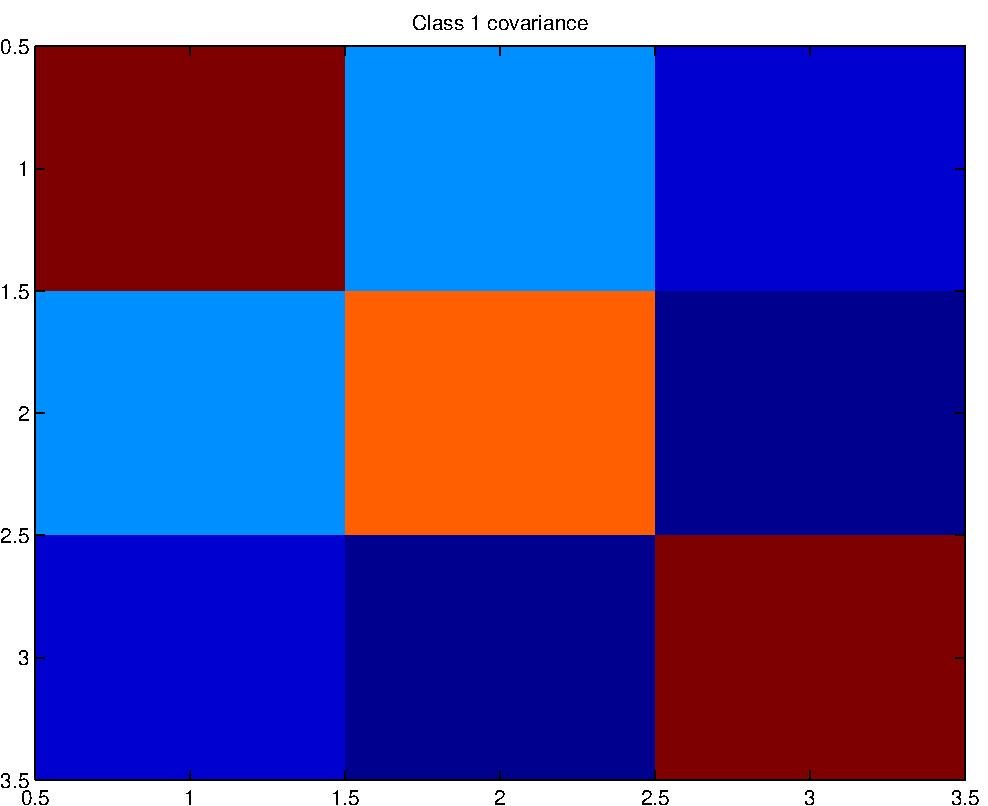
\includegraphics[width=10.0cm,height=10.0cm]{rv1_corr.pdf}

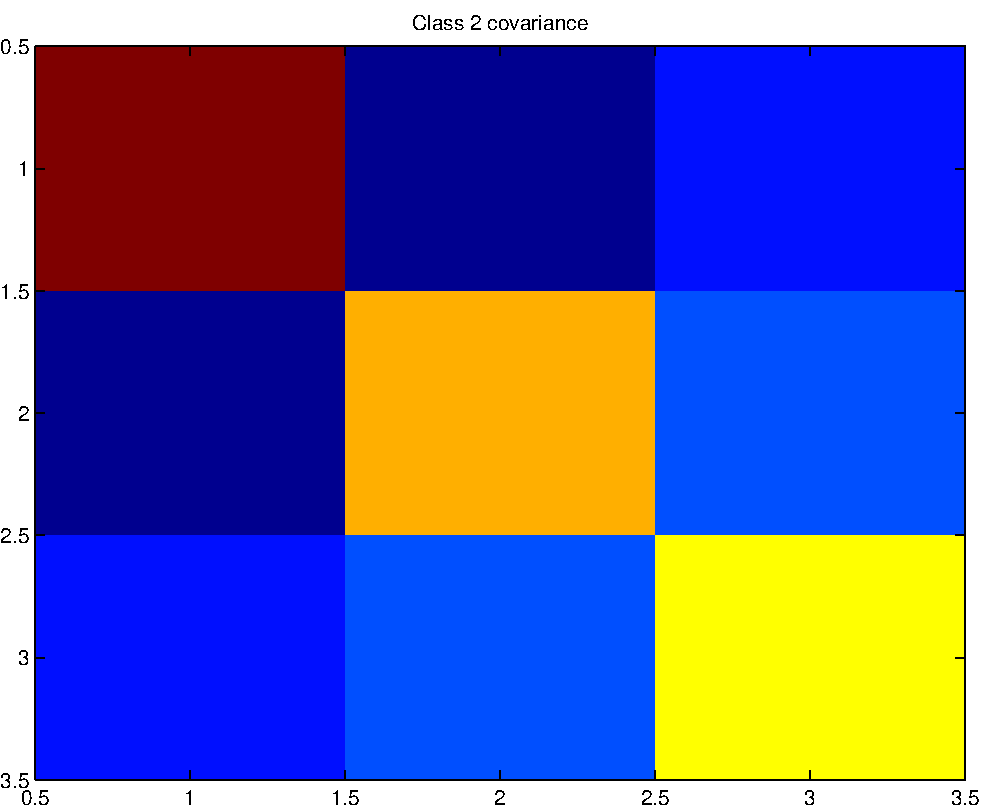
\includegraphics[width=10.0cm,height=10.0cm]{rv2_corr.pdf}

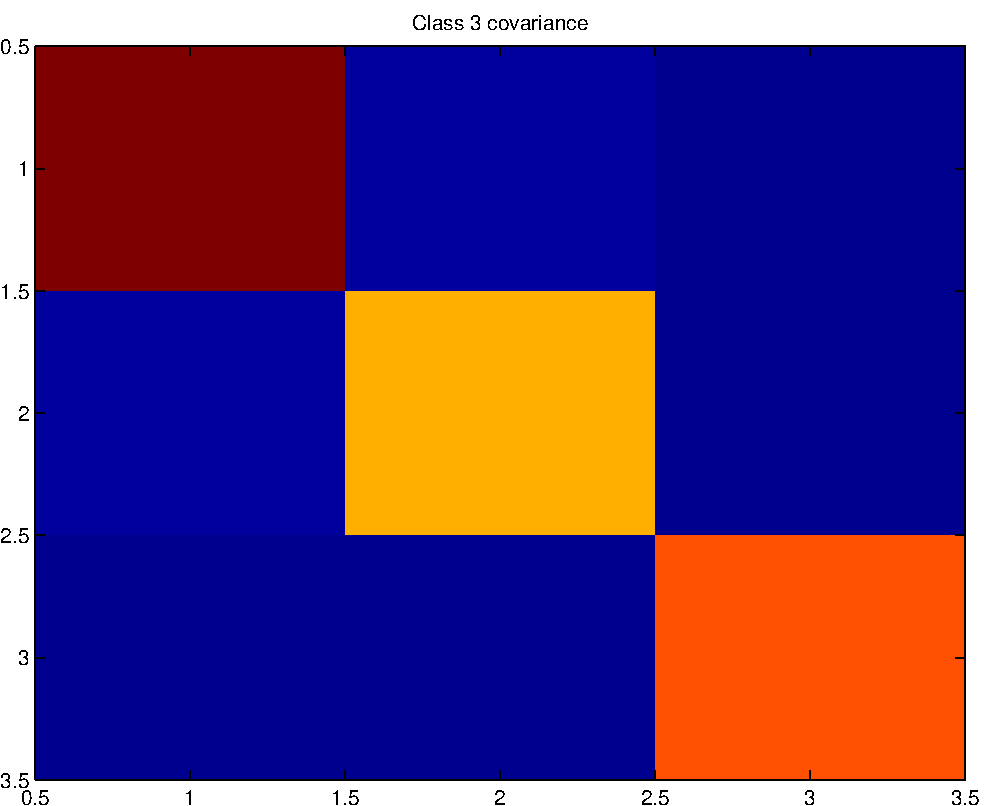
\includegraphics[width=10.0cm,height=10.0cm]{rv3_corr.pdf}

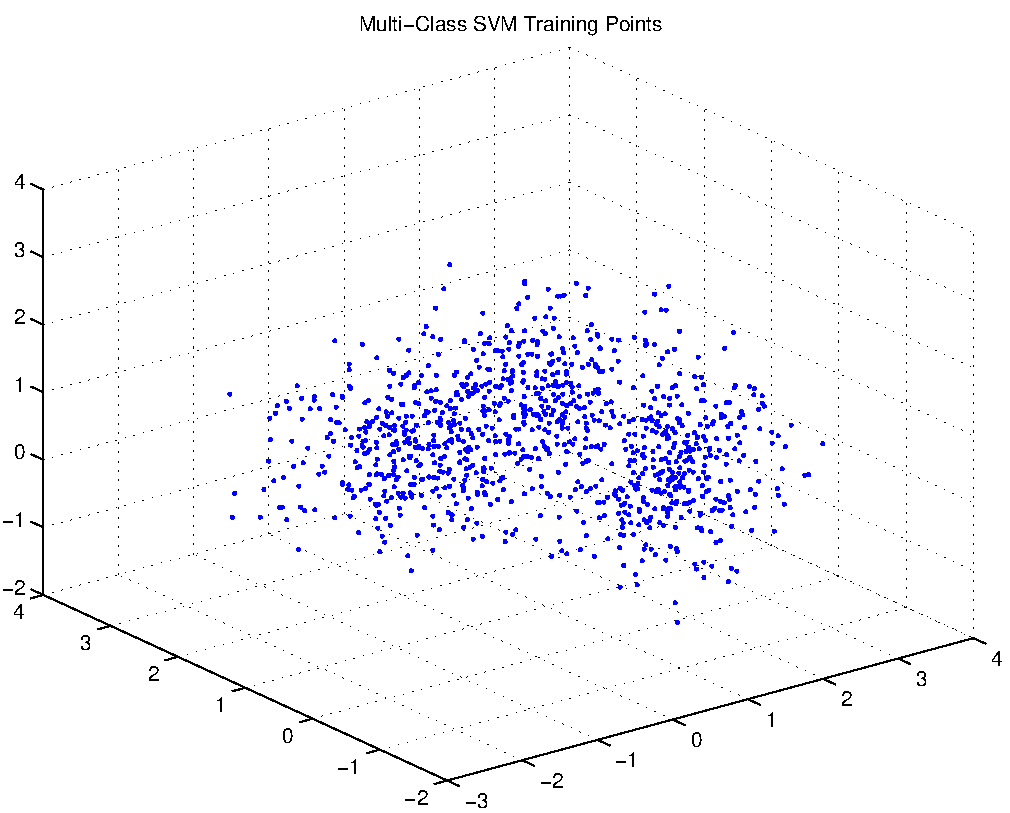
\includegraphics[width=10.0cm,height=10.0cm]{trainingPoints.pdf}

These are the SVM parameters - the RBF kernel is used\begin{itemize}
\item allOutlierFraction=0.05
\item mixingCoeff=0.3
\item smoThresh=1.0/10000.0
\item sigma=1
\end{itemize}
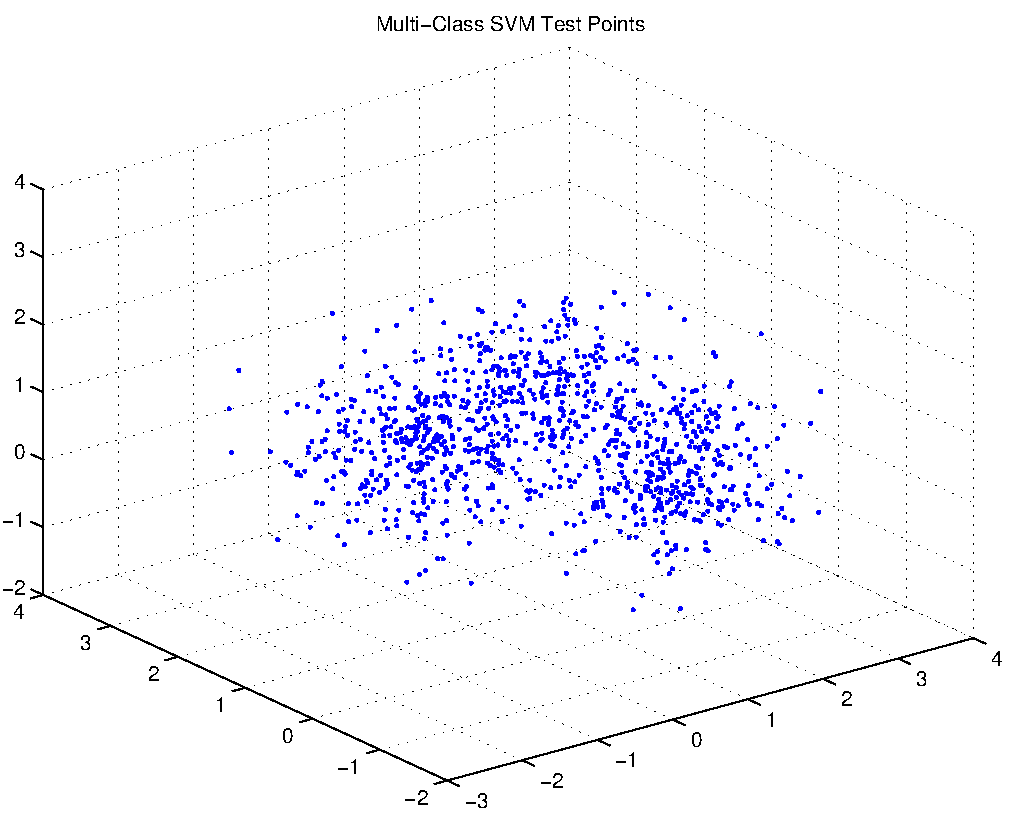
\includegraphics[width=10.0cm,height=10.0cm]{testPoints.pdf}

The marginal sample moments (mean var skew kurtosis) for training points.\newline
\begin{tabular}{ c |  c  c  c  c}
Feature & $\mu_1$ & $\mu_2$ & $\mu_3$ & $\mu_4$ \\
0 & +0.668 & +1.318 & +0.140& +2.247 \\
\hline
1 & +0.698 & +1.087 & +0.377& +2.155 \\
\hline
2 & +0.702 & +1.142 & +0.479& +2.438 \\
\hline
\end{tabular}
\newline
The marginal sample moments (mean var skew kurtosis) for test points.\newline
\begin{tabular}{ c | c  c  c  c}
Feature & $\mu_1$ & $\mu_2$ & $\mu_3$ & $\mu_4$ \\
0 & +0.676 & +1.222 & +0.275& +2.312\\
\hline
1 & +0.669 & +1.090 & +0.419& +2.173\\
\hline
2 & +0.720 & +1.081 & +0.480& +2.369\\
\hline
\end{tabular}\newline
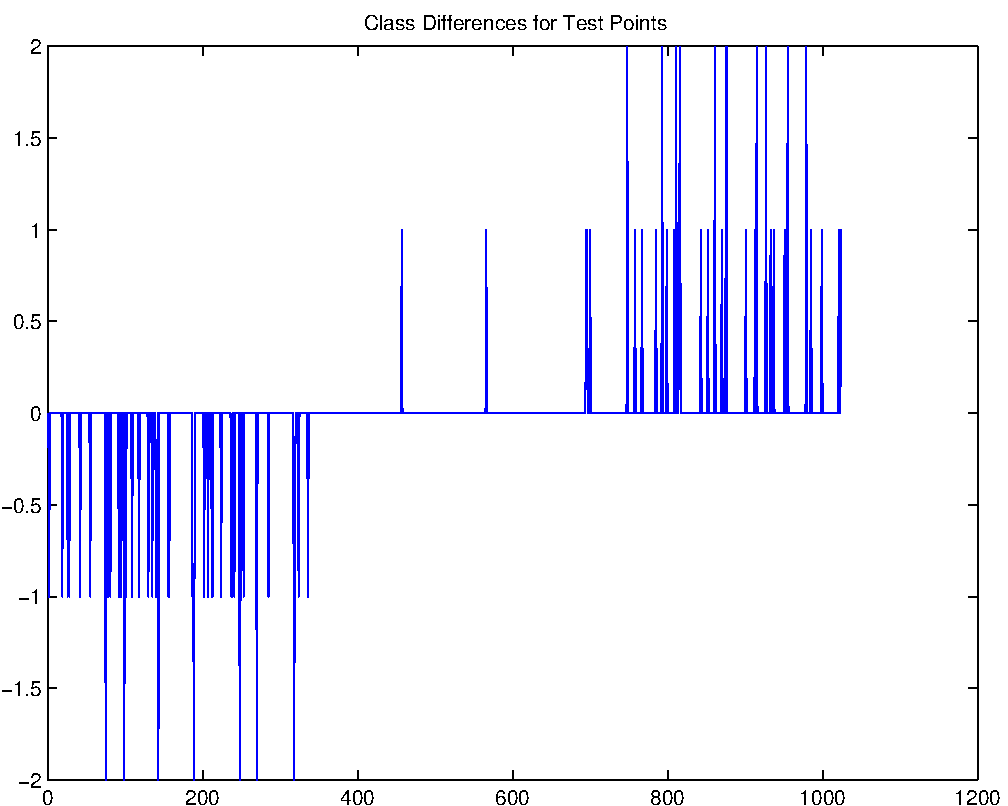
\includegraphics[width=10.0cm,height=10.0cm]{classDiffs.pdf}

The error rate for this run is +0.075\newline
QueryPerformanceCounter  =  +6.128
\subsubsection{Matrix Quick Check <double>}
QueryPerformanceCounter  =  +0.092
\subsubsection{Linear Regression atan data 3x1}
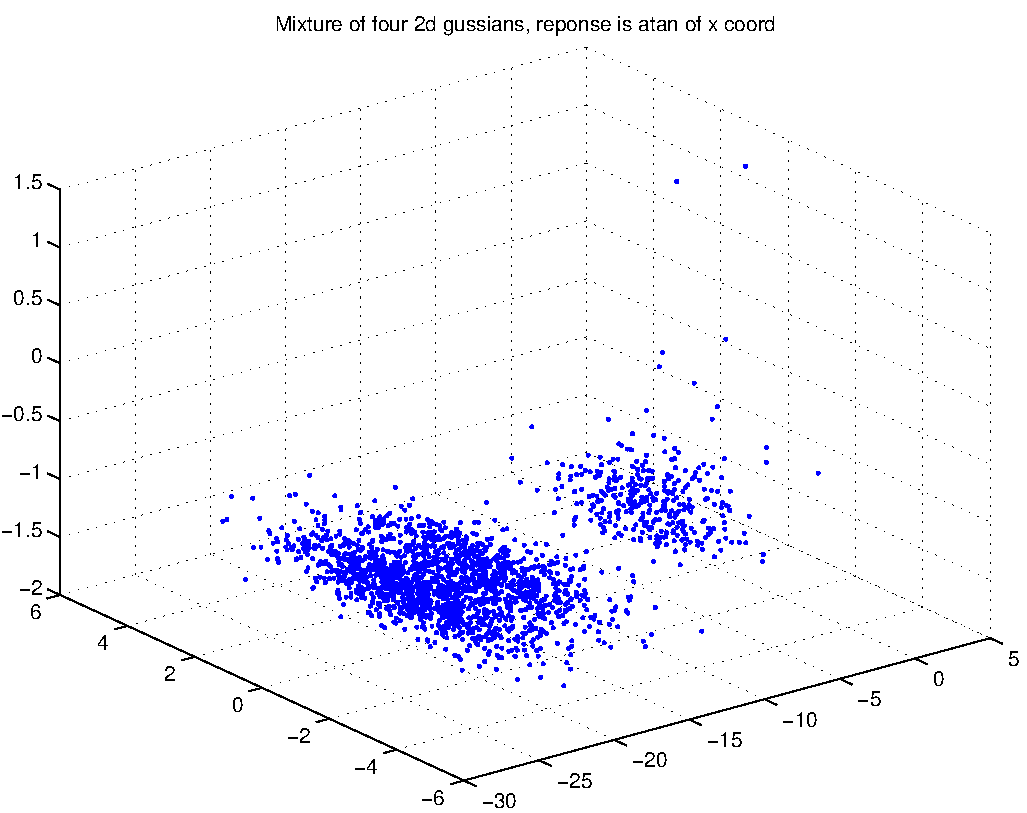
\includegraphics[width=10.0cm,height=10.0cm]{AtanDataSet.pdf}

\subsubsection{3 x 1 Linear Regression}
Sample size = 4000

Number of features = 3

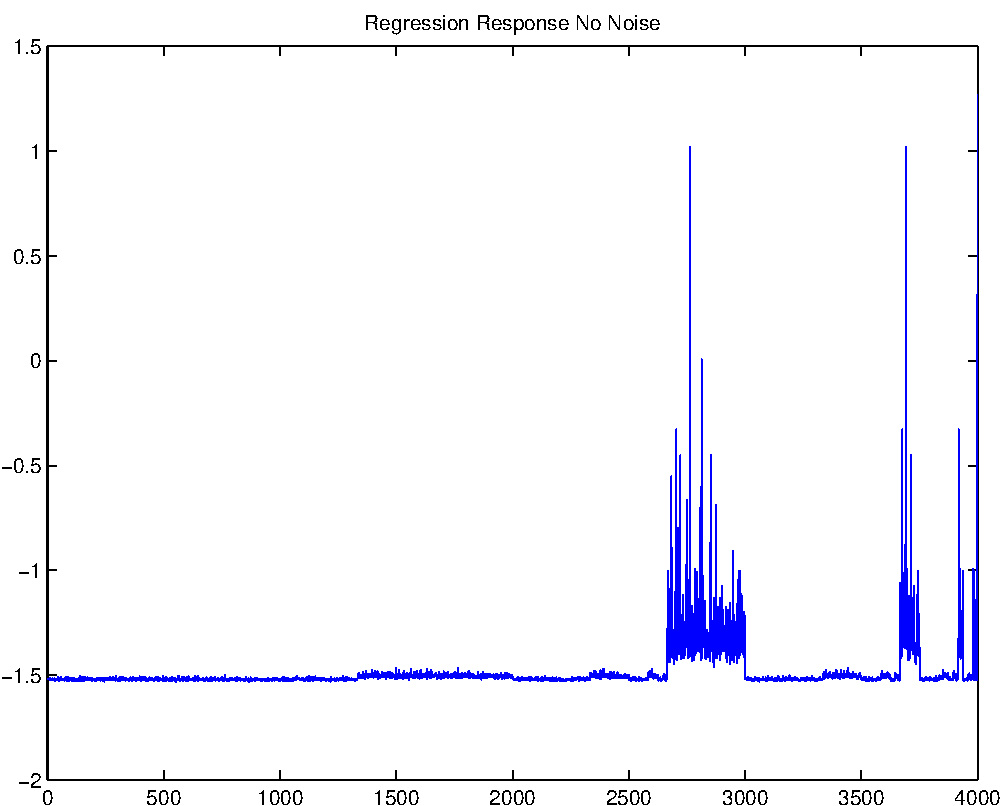
\includegraphics[width=10.0cm,height=10.0cm]{AtanDataSet_regression_response_no_noise.pdf}

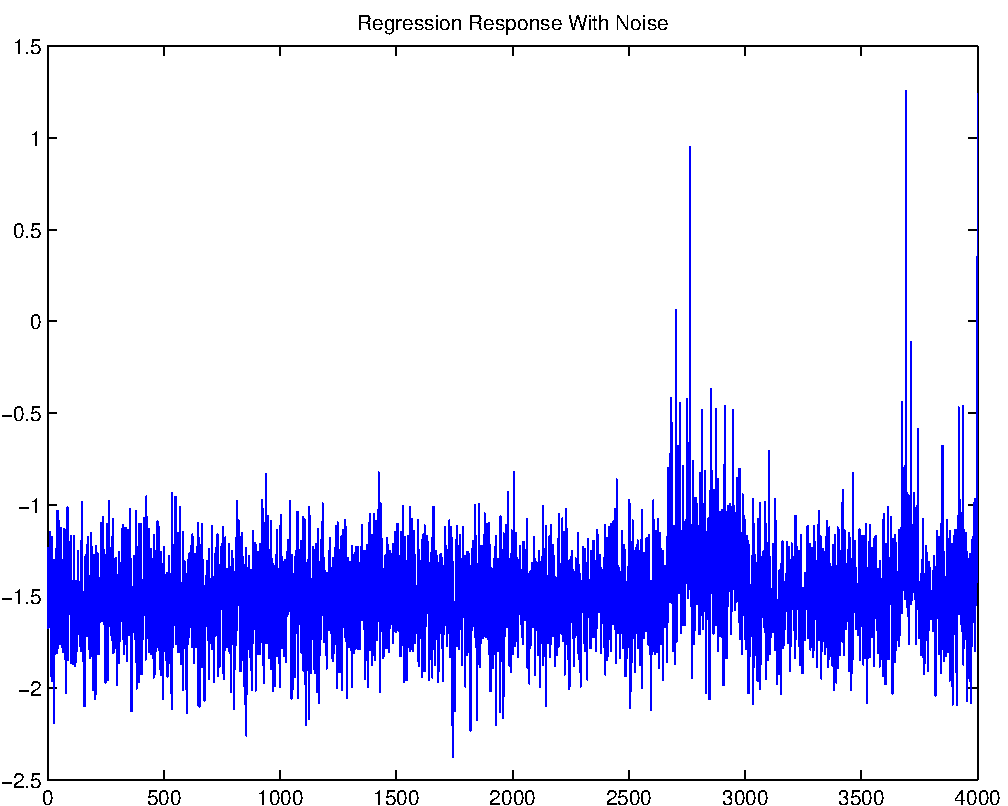
\includegraphics[width=10.0cm,height=10.0cm]{AtanDataSet_regression_response_with_noise.pdf}

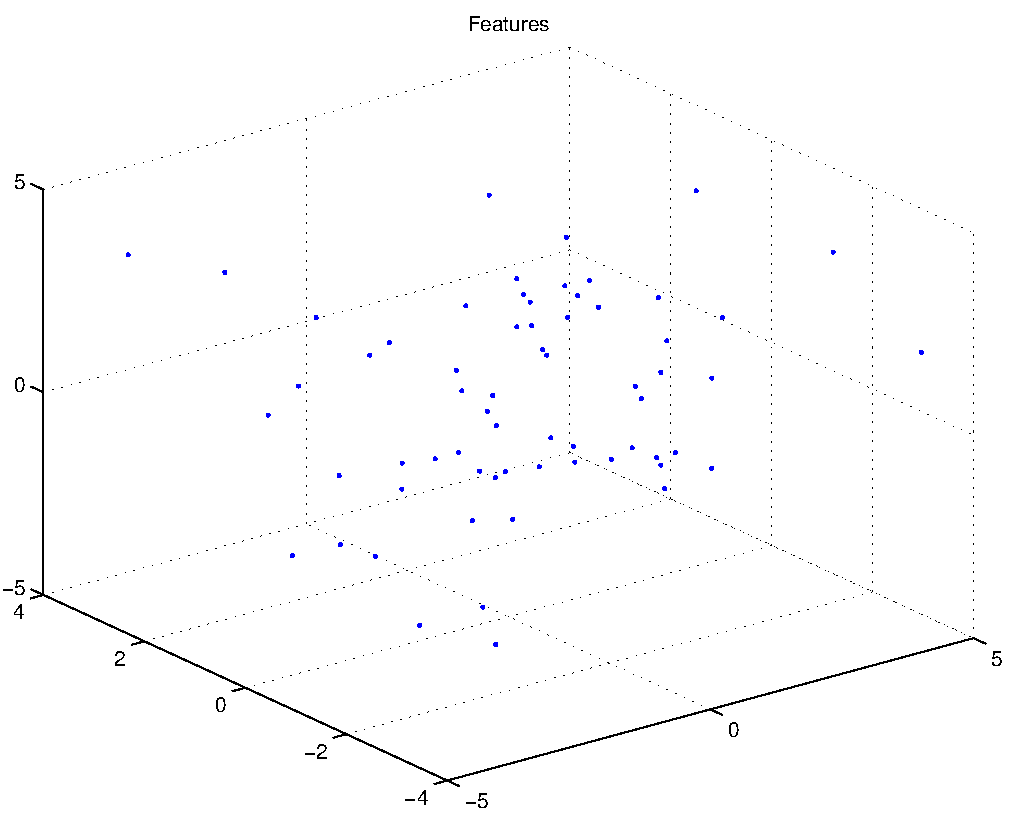
\includegraphics[width=10.0cm,height=10.0cm]{regression_features.pdf}

Response
-1.438
-1.670
-1.583
-1.236
-1.311
-1.349
-1.411
-1.285
-1.308
-1.147
-1.667
-1.377
-1.741
-1.505
-1.428
-1.935
-1.175
-1.378
-1.960
-1.597
-1.428
-1.544
-1.358
-1.863
-1.473
-2.193
-1.301
-1.391
-1.456
-1.768
-1.594
-1.354
-1.815
-1.795
-1.685
-1.241
-1.265
-1.502
-1.356
-1.813
-1.165
-1.384
-1.031
-1.250
-1.234
-1.780
-1.526
-1.701
-1.527
-1.089
-1.409
-1.281
-1.560
-1.760
-1.440
-1.664
-1.459
-1.127
-1.682
-1.679
-1.492
-1.775
-1.539
-1.649
-1.804
-1.300
-1.497
-1.709
-1.535
-1.499
-1.184
-1.132
-1.748
-1.238
-1.669
-1.843
-1.608
-2.026
-1.139
-1.595
-1.445
-1.537
-1.656
-1.038
-1.337
-1.013
-1.636
-1.497
-1.849
-1.561
-1.525
-1.385
-1.382
-1.536
-1.400
-1.593
-1.375
-1.236
-1.168
-1.865
-1.830
-1.524
-1.622
-1.832
-1.706
-1.841
-1.414
-1.494
-1.622
-1.628
-1.868
-1.446
-1.173
-1.380
-1.764
-1.610
-1.811
-1.416
-1.878
-1.558
-1.675
-1.627
-1.858
-1.733
-1.800
-1.563
-1.715
-1.457
-1.420
-1.252
-1.681
-1.611
-1.703
-1.664
-1.552
-1.521
-1.572
-1.770
-1.711
-1.421
-1.650
-1.456
-1.290
-1.772
-1.799
-1.196
-1.736
-0.986
-1.629
-1.778
-1.854
-1.533
-1.476
-1.737
-1.563
-1.652
-1.677
-1.484
-2.099
-1.706
-1.383
-1.302
-1.284
-1.430
-1.682
-1.597
-1.341
-1.220
-1.716
-1.502
-1.386
-1.472
-1.376
-1.189
-1.173
-1.531
-1.630
-1.786
-1.496
-1.386
-1.488
-1.591
-1.834
-1.596
-1.483
-1.827
-1.151
-1.218
-1.556
-1.458
-1.762
-1.231
-1.739
-1.389
-1.474
-1.420
-2.011
-1.412
-1.551
-1.628
-1.274
-1.366
-2.058
-1.745
-1.346
-1.414
-2.030
-1.405
-1.463
-1.225
-1.544
-1.281
-1.612
-1.740
-1.264
-1.394
-1.517
-1.816
-1.738
-1.520
-1.813
-1.429
-1.617
-1.496
-1.439
-1.397
-1.642
-1.546
-1.542
-1.099
-1.448
-1.378
-1.398
-1.173
-1.624
-1.635
-1.509
-1.431
-1.415
-1.065
-1.483
-1.535
-1.652
-1.639
-1.325
-1.736
-1.276
-1.450
-1.970
-1.514
-1.505
-1.433
-1.425
-1.364
-1.106
-1.547
-1.333
-1.578
-1.334
-1.952
-1.957
-1.477
-0.980
-1.329
-1.661
-1.197
-1.385
-1.233
-1.565
-1.623
-1.492
-1.262
-1.623
-1.442
-1.712
-1.444
-1.194
-1.736
-1.173
-1.808
-1.350
-1.460
-1.076
-1.804
-1.646
-1.600
-1.704
-1.564
-1.510
-1.355
-1.296
-1.779
-1.445
-1.291
-1.571
-1.516
-1.421
-1.487
-1.984
-1.972
-1.381
-1.456
-1.593
-1.538
-1.674
-1.609
-1.257
-1.865
-1.449
-1.742
-1.318
-1.423
-1.634
-1.324
-1.538
-1.570
-1.590
-1.504
-1.402
-1.131
-1.495
-1.514
-1.733
-1.403
-1.108
-1.584
-1.579
-1.815
-1.416
-1.608
-1.599
-1.422
-1.422
-1.565
-1.125
-1.651
-1.418
-1.204
-1.758
-1.285
-1.423
-1.179
-1.851
-1.321
-1.135
-1.628
-1.649
-1.707
-1.410
-1.432
-1.712
-1.373
-1.466
-1.257
-1.021
-1.078
-1.596
-1.493
-1.565
-1.501
-2.124
-1.449
-1.951
-1.533
-1.451
-1.685
-1.479
-1.624
-1.603
-1.689
-1.278
-1.501
-1.520
-1.694
-1.573
-1.462
-1.584
-1.723
-1.833
-1.036
-1.856
-1.371
-2.003
-1.794
-1.591
-1.624
-1.232
-1.721
-1.244
-1.358
-1.367
-1.966
-1.776
-1.107
-1.696
-1.268
-1.617
-1.877
-1.598
-1.376
-1.105
-1.623
-1.577
-1.923
-1.672
-1.551
-1.655
-1.544
-1.591
-1.483
-1.730
-1.407
-1.498
-1.451
-1.602
-1.294
-1.071
-1.332
-1.299
-1.525
-1.500
-1.844
-1.611
-1.247
-0.955
-1.586
-1.068
-1.724
-1.259
-1.442
-1.423
-1.199
-1.175
-1.377
-1.132
-1.563
-1.802
-1.689
-1.488
-1.402
-1.569
-1.592
-1.681
-1.312
-1.243
-1.395
-1.814
-1.295
-1.315
-1.460
-1.395
-1.319
-1.833
-1.645
-1.508
-1.943
-1.163
-1.233
-1.345
-1.630
-1.902
-1.546
-1.922
-1.772
-1.249
-1.739
-1.797
-1.541
-1.536
-1.203
-1.426
-1.662
-1.091
-1.163
-1.678
-1.779
-1.388
-1.122
-1.529
-1.793
-1.241
-1.714
-1.894
-1.337
-1.719
-1.519
-1.397
-1.258
-1.930
-1.458
-1.622
-1.538
-1.496
-1.523
-1.370
-1.437
-2.056
-1.324
-1.801
-1.601
-1.231
-1.289
-1.732
-1.505
-1.785
-1.581
-1.382
-1.518
-1.847
-1.419
-1.537
-1.504
-1.820
-1.617
-1.370
-1.937
-1.776
-1.526
-1.373
-1.417
-1.278
-1.799
-1.481
-1.762
-1.865
-1.769
-1.859
-1.456
-1.380
-1.501
-1.381
-2.028
-1.405
-1.479
-0.930
-1.572
-2.113
-1.333
-1.391
-1.218
-1.425
-1.306
-1.436
-1.653
-1.486
-1.440
-1.523
-1.423
-1.472
-0.956
-1.317
-1.723
-1.760
-1.543
-1.642
-1.485
-1.622
-1.396
-1.428
-1.447
-1.458
-1.151
-1.802
-1.530
-1.732
-1.458
-1.498
-1.616
-1.015
-1.560
-1.629
-1.501
-1.871
-1.667
-1.427
-1.831
-1.555
-1.556
-1.696
-1.640
-2.009
-1.334
-1.149
-1.699
-1.500
-1.536
-1.662
-1.383
-1.309
-1.473
-1.415
-1.784
-1.494
-1.594
-1.512
-1.376
-1.848
-2.137
-1.894
-1.534
-1.733
-1.515
-1.400
-1.735
-1.756
-1.298
-1.349
-1.612
-1.720
-1.265
-1.657
-1.664
-1.415
-1.437
-1.662
-1.297
-1.223
-1.505
-1.467
-1.775
-1.185
-1.275
-1.161
-1.186
-1.524
-1.341
-1.356
-1.536
-1.320
-1.862
-1.744
-1.654
-1.269
-1.683
-1.283
-1.289
-1.460
-1.774
-1.452
-1.361
-1.765
-1.275
-1.232
-1.304
-1.516
-1.761
-1.740
-1.100
-2.095
-1.271
-1.526
-1.640
-1.180
-2.100
-1.220
-1.546
-1.431
-1.565
-1.695
-1.590
-1.440
-1.705
-1.383
-1.885
-1.106
-1.294
-1.728
-1.303
-1.315
-1.624
-1.693
-1.671
-1.442
-1.761
-2.068
-1.578
-1.820
-1.840
-1.772
-1.388
-1.630
-1.663
-1.488
-1.322
-1.467
-1.423
-1.341
-1.306
-1.739
-1.490
-1.360
-1.307
-1.950
-1.241
-1.505
-1.670
-1.433
-1.728
-1.752
-1.731
-1.404
-1.567
-1.748
-1.612
-1.424
-1.410
-1.483
-1.116
-1.787
-1.404
-1.637
-1.579
-1.717
-1.393
-1.967
-1.834
-1.410
-1.676
-1.286
-1.713
-1.485
-1.310
-1.234
-1.476
-1.520
-1.417
-1.613
-1.711
-1.285
-1.552
-1.161
-1.932
-1.529
-1.423
-1.326
-1.527
-1.536
-1.600
-1.709
-1.882
-1.333
-1.746
-1.510
-1.438
-1.272
-1.568
-1.505
-1.228
-1.451
-1.404
-1.216
-1.553
-1.433
-1.919
-1.308
-1.119
-1.525
-1.852
-1.513
-1.952
-1.337
-1.646
-1.433
-1.790
-1.177
-1.647
-1.769
-1.459
-1.542
-1.667
-1.350
-1.687
-1.776
-1.521
-1.674
-1.688
-1.739
-1.435
-1.751
-1.214
-1.328
-1.799
-1.589
-1.337
-1.810
-1.508
-1.557
-1.540
-2.020
-1.483
-1.645
-1.760
-1.648
-1.713
-1.252
-1.745
-1.523
-1.294
-1.452
-1.840
-1.412
-1.808
-2.112
-1.878
-1.414
-1.650
-1.363
-1.871
-1.183
-1.202
-1.300
-1.766
-1.572
-1.577
-0.978
-1.493
-1.338
-1.392
-1.547
-1.326
-1.084
-1.510
-1.522
-1.388
-1.470
-1.330
-1.794
-1.505
-1.556
-1.908
-1.523
-1.460
-1.177
-1.469
-1.468
-1.496
-1.151
-1.310
-1.494
-1.845
-1.446
-1.284
-1.641
-1.630
-1.986
-1.326
-1.502
-1.539
-2.086
-1.585
-1.825
-1.233
-1.622
-1.593
-2.259
-1.736
-1.802
-1.424
-1.344
-1.638
-1.533
-1.765
-1.787
-1.597
-1.473
-1.316
-1.694
-1.278
-1.654
-1.829
-1.538
-1.457
-1.679
-1.357
-1.680
-1.900
-1.691
-1.514
-1.807
-1.545
-2.010
-1.143
-1.511
-1.754
-1.343
-1.415
-1.631
-1.679
-1.654
-1.321
-1.517
-1.270
-1.571
-1.207
-2.014
-1.430
-1.464
-1.222
-1.688
-1.285
-1.801
-1.637
-1.291
-1.276
-1.815
-1.793
-1.256
-1.609
-1.601
-1.384
-1.750
-1.475
-1.294
-1.216
-1.816
-1.486
-1.548
-1.488
-1.749
-1.720
-1.390
-0.975
-1.611
-1.243
-1.574
-1.446
-1.021
-1.701
-1.875
-1.718
-1.972
-1.788
-1.753
-1.597
-1.307
-1.479
-1.100
-1.412
-1.408
-1.724
-0.830
-1.752
-1.385
-1.420
-1.557
-1.555
-1.061
-1.604
-1.509
-1.460
-1.838
-1.515
-1.397
-1.245
-1.349
-1.289
-1.827
-1.682
-1.467
-1.554
-1.898
-1.086
-1.595
-1.292
-1.689
-1.334
-1.785
-1.319
-1.689
-1.397
-2.017
-1.814
-1.597
-1.731
-1.478
-1.988
-1.559
-1.656
-1.334
-1.502
-1.273
-1.455
-1.572
-1.524
-1.136
-1.262
-1.825
-1.587
-1.481
-1.449
-1.457
-1.574
-1.348
-1.401
-1.865
-1.360
-1.601
-1.196
-1.114
-1.575
-1.996
-1.670
-1.056
-1.742
-1.610
-1.612
-1.286
-1.408
-1.783
-1.337
-1.607
-1.561
-1.361
-1.479
-1.314
-1.312
-1.826
-1.465
-1.553
-1.313
-1.303
-1.686
-1.349
-1.461
-1.558
-1.552
-1.859
-1.259
-1.547
-1.462
-1.529
-1.475
-1.408
-1.597
-1.192
-1.585
-1.261
-1.461
-1.233
-1.283
-1.510
-1.480
-1.572
-0.977
-1.582
-1.531
-1.634
-1.433
-2.057
-1.597
-1.807
-1.272
-1.449
-2.008
-1.729
-1.646
-1.733
-1.429
-1.560
-1.551
-1.379
-1.407
-1.477
-1.606
-1.936
-1.329
-1.250
-1.563
-1.399
-1.271
-1.321
-1.190
-1.698
-1.373
-1.038
-2.053
-1.835
-1.523
-1.410
-1.493
-1.490
-1.650
-1.245
-1.481
-1.609
-1.648
-1.590
-1.364
-1.385
-1.464
-1.196
-1.807
-1.496
-1.450
-1.597
-1.345
-1.288
-1.354
-1.772
-1.067
-1.905
-1.349
-1.327
-1.807
-1.079
-1.795
-1.367
-1.978
-1.533
-1.319
-2.200
-1.748
-1.544
-1.508
-1.784
-1.332
-1.319
-1.900
-1.568
-1.859
-1.542
-1.298
-1.683
-2.165
-1.011
-1.589
-1.062
-1.526
-1.787
-1.597
-1.918
-1.625
-1.497
-1.871
-1.481
-1.639
-1.407
-1.562
-1.575
-1.734
-1.367
-1.229
-1.345
-1.493
-1.648
-1.249
-1.501
-1.896
-1.394
-1.495
-1.918
-1.506
-1.357
-1.813
-1.214
-1.630
-1.644
-1.311
-1.240
-2.021
-1.767
-1.133
-1.732
-1.952
-1.746
-2.082
-1.866
-1.318
-1.595
-1.559
-1.313
-1.820
-1.480
-1.364
-1.732
-1.500
-1.189
-1.589
-1.239
-1.380
-1.598
-1.228
-0.992
-1.545
-1.335
-1.426
-1.568
-1.747
-1.540
-1.293
-1.360
-1.443
-1.633
-1.605
-1.560
-1.385
-1.736
-1.730
-1.724
-1.893
-1.370
-1.485
-1.706
-1.460
-1.451
-1.529
-1.483
-1.556
-1.519
-1.480
-1.682
-1.330
-1.182
-1.351
-1.367
-1.389
-1.621
-1.346
-1.467
-1.702
-1.654
-1.833
-1.489
-1.585
-1.774
-1.719
-1.290
-1.856
-1.288
-1.386
-1.810
-1.515
-1.459
-1.453
-1.684
-1.233
-1.524
-1.357
-1.325
-1.760
-1.173
-1.304
-1.116
-1.365
-2.000
-1.413
-1.486
-1.096
-1.550
-1.476
-1.785
-1.910
-1.627
-1.618
-1.691
-1.351
-1.250
-1.664
-1.248
-1.889
-1.674
-1.175
-1.676
-1.901
-2.011
-1.502
-1.168
-1.204
-1.445
-1.455
-1.140
-1.614
-1.664
-1.641
-1.367
-1.599
-1.603
-1.651
-1.500
-1.721
-1.080
-1.740
-1.433
-1.119
-1.326
-1.714
-1.652
-2.051
-1.495
-1.354
-1.750
-1.291
-1.393
-1.554
-1.777
-1.602
-1.559
-1.718
-1.365
-1.730
-1.536
-1.313
-1.641
-1.523
-1.614
-1.643
-1.791
-1.222
-1.994
-1.599
-1.262
-1.377
-1.507
-1.271
-1.491
-1.291
-1.454
-1.810
-1.395
-1.708
-1.731
-1.293
-1.262
-1.785
-1.757
-1.230
-1.531
-1.703
-1.673
-1.678
-1.519
-1.457
-1.780
-1.232
-1.784
-1.780
-1.557
-1.471
-1.376
-1.377
-1.657
-1.536
-1.657
-1.788
-1.427
-1.318
-1.415
-1.591
-1.259
-1.229
-1.473
-1.107
-1.630
-1.382
-1.614
-1.328
-1.357
-1.304
-1.332
-1.253
-1.511
-1.680
-1.356
-1.866
-1.949
-1.252
-1.838
-1.682
-1.506
-1.609
-1.846
-1.459
-1.535
-1.220
-1.333
-1.347
-1.993
-1.679
-1.414
-1.529
-1.631
-1.098
-1.506
-1.295
-1.532
-1.343
-1.792
-1.050
-1.169
-1.169
-1.634
-1.565
-1.548
-1.315
-1.872
-1.298
-1.334
-1.631
-1.163
-1.820
-1.188
-1.430
-1.575
-1.588
-1.051
-1.810
-1.845
-1.239
-1.674
-1.373
-1.086
-1.476
-1.353
-1.117
-1.548
-1.414
-1.735
-1.157
-1.524
-1.561
-1.354
-1.470
-1.303
-0.823
-1.312
-1.555
-1.634
-1.527
-1.718
-1.230
-2.020
-1.507
-0.993
-1.357
-1.420
-1.389
-1.690
-1.530
-1.186
-1.611
-1.370
-1.837
-1.383
-1.353
-1.433
-1.481
-1.827
-1.348
-1.742
-1.727
-1.472
-1.782
-1.276
-1.604
-1.488
-1.442
-1.648
-1.779
-1.495
-1.182
-1.714
-1.497
-1.218
-1.780
-1.473
-1.417
-1.658
-1.804
-1.324
-1.312
-1.633
-1.251
-1.623
-1.674
-1.582
-1.295
-1.438
-1.652
-1.276
-1.517
-1.303
-1.266
-1.532
-1.428
-1.753
-1.417
-1.325
-1.214
-1.512
-1.479
-1.300
-1.566
-1.146
-1.347
-1.667
-1.687
-1.283
-1.510
-1.593
-1.696
-1.420
-1.103
-1.504
-1.180
-1.234
-1.596
-1.103
-1.542
-1.687
-1.279
-1.385
-1.643
-1.620
-1.516
-1.380
-1.474
-1.548
-1.824
-1.547
-1.502
-1.148
-1.354
-1.164
-1.661
-1.643
-1.600
-1.423
-1.004
-1.408
-1.502
-1.764
-1.449
-1.965
-1.336
-1.337
-1.851
-1.553
-1.176
-1.633
-1.691
-1.306
-1.549
-1.420
-1.956
-1.357
-1.599
-1.486
-1.385
-1.774
-1.339
-1.172
-1.637
-1.198
-1.428
-1.193
-1.425
-1.797
-1.010
-1.755
-1.460
-1.580
-1.572
-1.788
-1.722
-1.104
-1.280
-1.322
-1.077
-1.416
-1.489
-1.796
-1.453
-1.572
-1.628
-1.622
-1.141
-1.327
-1.271
-1.516
-1.634
-1.756
-1.672
-1.531
-1.526
-1.662
-1.681
-1.656
-1.522
-1.443
-1.487
-1.702
-1.433
-1.850
-1.080
-1.367
-1.788
-1.599
-1.245
-1.881
-1.515
-1.725
-1.358
-1.634
-1.603
-1.309
-1.519
-1.693
-1.584
-1.256
-1.939
-1.192
-1.390
-1.585
-1.466
-1.718
-1.710
-1.161
-1.481
-1.494
-1.255
-1.908
-1.112
-1.452
-1.615
-1.626
-1.441
-1.661
-1.516
-1.575
-1.483
-1.170
-1.492
-1.466
-1.201
-1.589
-1.232
-1.348
-1.338
-1.316
-1.518
-1.954
-1.749
-1.555
-1.483
-1.444
-1.656
-1.842
-1.844
-1.519
-1.588
-1.375
-1.180
-1.593
-1.431
-1.942
-1.560
-1.789
-1.593
-1.724
-1.010
-1.387
-1.393
-1.761
-1.405
-1.675
-1.873
-1.307
-1.724
-1.736
-1.254
-1.673
-1.269
-1.275
-1.608
-1.451
-1.282
-1.490
-1.650
-1.470
-1.966
-1.625
-1.317
-1.482
-1.904
-1.745
-1.491
-1.526
-1.276
-1.594
-1.348
-1.302
-1.646
-1.698
-1.268
-1.309
-1.778
-1.705
-1.758
-1.697
-1.962
-1.440
-1.525
-1.566
-1.334
-1.703
-1.640
-1.636
-1.545
-1.122
-1.351
-1.499
-1.555
-1.473
-1.227
-1.655
-1.261
-1.590
-1.247
-1.770
-1.348
-1.257
-1.343
-1.335
-1.276
-1.697
-1.182
-1.480
-1.085
-1.554
-1.301
-1.210
-1.828
-1.690
-1.657
-1.119
-1.575
-1.448
-1.628
-1.545
-1.182
-1.961
-2.374
-1.313
-1.461
-1.781
-1.988
-1.657
-1.529
-1.533
-1.735
-1.634
-1.709
-2.125
-2.015
-1.322
-1.192
-1.545
-1.500
-1.435
-1.770
-1.404
-1.117
-1.631
-1.391
-1.700
-1.745
-1.643
-1.788
-1.362
-1.633
-1.490
-1.228
-1.166
-1.186
-1.351
-1.368
-1.642
-1.583
-1.307
-1.432
-1.864
-1.622
-1.871
-1.411
-1.209
-1.119
-1.437
-1.454
-1.513
-1.456
-1.609
-1.534
-1.371
-1.453
-1.366
-1.281
-1.992
-1.321
-1.733
-1.597
-1.661
-1.490
-1.571
-1.577
-1.820
-1.255
-1.513
-1.476
-1.373
-1.794
-1.268
-1.526
-1.414
-1.644
-1.803
-1.336
-1.640
-1.871
-2.231
-1.443
-1.563
-1.359
-1.638
-1.241
-1.344
-1.685
-1.566
-1.411
-1.655
-1.198
-1.437
-1.264
-1.664
-1.627
-1.529
-1.567
-1.708
-1.001
-1.694
-1.722
-1.268
-1.167
-1.491
-1.779
-1.679
-1.715
-1.585
-2.172
-1.340
-1.325
-1.842
-1.682
-1.482
-1.407
-1.557
-0.995
-1.869
-1.525
-1.259
-1.440
-1.886
-1.748
-1.320
-1.224
-1.538
-1.430
-1.480
-1.662
-1.276
-1.431
-1.726
-1.536
-1.353
-1.226
-1.304
-1.263
-1.510
-1.466
-1.313
-1.047
-1.594
-1.434
-1.714
-1.206
-1.517
-1.360
-1.719
-1.565
-1.498
-1.107
-1.354
-1.648
-1.456
-1.733
-1.329
-1.467
-1.100
-1.811
-1.512
-1.209
-1.219
-1.733
-1.792
-1.807
-2.016
-1.574
-1.502
-1.415
-1.628
-1.347
-1.470
-1.864
-1.375
-1.645
-1.888
-1.424
-1.626
-1.656
-1.618
-1.294
-1.337
-1.686
-1.363
-1.232
-1.383
-1.706
-1.893
-1.567
-2.201
-1.169
-1.608
-1.496
-1.715
-1.384
-1.552
-1.645
-1.367
-1.294
-1.799
-1.471
-1.685
-1.633
-1.679
-1.507
-2.129
-1.467
-1.356
-1.063
-1.306
-1.263
-1.282
-1.154
-1.377
-1.631
-1.395
-1.434
-2.162
-1.826
-1.625
-1.247
-1.274
-1.156
-2.040
-1.613
-1.248
-1.719
-1.694
-1.643
-1.271
-1.309
-1.111
-1.389
-1.507
-1.315
-1.379
-1.505
-1.669
-1.380
-1.545
-1.470
-0.933
-1.603
-1.294
-1.758
-1.414
-1.720
-1.876
-1.763
-1.486
-1.408
-1.352
-1.912
-1.304
-1.331
-1.439
-1.140
-1.455
-1.439
-1.184
-1.686
-1.290
-1.814
-1.758
-1.564
-0.820
-1.517
-0.915
-1.541
-1.772
-1.378
-1.537
-1.676
-1.152
-1.335
-1.408
-1.409
-1.743
-1.341
-1.290
-1.675
-1.663
-1.829
-1.449
-1.629
-1.551
-1.493
-1.547
-1.450
-1.298
-1.598
-1.467
-1.226
-1.582
-1.441
-1.353
-1.529
-1.560
-1.652
-1.366
-1.389
-1.451
-1.721
-1.639
-1.684
-1.757
-1.292
-1.201
-1.515
-1.432
-1.456
-1.629
-1.429
-1.308
-1.595
-1.440
-1.547
-1.450
-1.621
-1.628
-1.245
-1.704
-1.075
-1.406
-1.888
-1.426
-1.746
-1.739
-1.801
-1.508
-1.376
-1.532
-1.975
-1.432
-1.782
-1.708
-1.363
-1.536
-1.372
-1.762
-1.531
-1.552
-1.349
-1.317
-1.566
-1.505
-1.570
-1.666
-1.382
-1.405
-1.444
-1.393
-1.177
-1.299
-1.267
-1.333
-1.929
-1.782
-1.799
-1.366
-1.477
-1.370
-1.590
-1.314
-1.491
-1.353
-1.686
-1.559
-1.558
-1.503
-1.820
-1.812
-1.252
-1.635
-1.683
-1.511
-1.807
-1.995
-1.310
-1.663
-1.315
-1.585
-1.421
-1.753
-1.529
-1.284
-1.649
-1.301
-1.345
-1.312
-1.876
-1.005
-1.486
-1.320
-1.463
-1.353
-1.241
-1.461
-1.497
-1.369
-1.827
-1.631
-1.535
-1.117
-2.097
-1.693
-1.425
-1.541
-1.633
-1.680
-1.418
-1.755
-1.644
-1.440
-1.468
-1.329
-1.483
-1.395
-1.495
-1.173
-1.464
-1.534
-1.828
-1.470
-1.185
-1.761
-1.109
-1.272
-1.706
-1.680
-1.372
-1.220
-1.306
-1.220
-1.660
-1.716
-1.274
-1.511
-1.423
-1.586
-1.431
-1.880
-1.582
-1.419
-1.708
-1.395
-1.556
-1.614
-1.751
-1.479
-1.502
-1.688
-1.695
-1.818
-1.665
-1.411
-1.561
-1.186
-1.774
-1.277
-1.053
-1.751
-1.447
-1.699
-1.416
-1.414
-1.396
-1.435
-1.654
-1.560
-1.548
-1.155
-1.522
-1.229
-1.074
-1.705
-1.576
-1.495
-1.744
-1.652
-1.470
-1.366
-1.689
-1.147
-1.925
-1.724
-1.615
-1.443
-1.453
-1.422
-1.021
-1.623
-1.295
-1.649
-1.458
-1.129
-1.760
-1.680
-1.787
-1.305
-1.623
-2.005
-1.673
-1.387
-1.352
-1.338
-1.987
-1.384
-1.342
-1.296
-1.322
-1.285
-1.510
-1.527
-1.457
-1.254
-1.309
-1.639
-1.360
-1.352
-1.689
-1.628
-1.729
-1.694
-1.880
-1.471
-1.740
-1.704
-1.366
-1.544
-1.531
-1.292
-1.548
-1.649
-1.711
-1.580
-1.342
-1.496
-1.401
-1.501
-1.153
-1.720
-1.760
-1.779
-1.839
-1.642
-1.331
-1.588
-1.591
-1.910
-1.376
-1.708
-1.819
-1.991
-1.418
-1.520
-1.522
-1.537
-1.504
-1.587
-1.515
-1.448
-1.537
-1.334
-1.229
-1.238
-1.258
-1.754
-1.249
-1.489
-1.400
-1.797
-1.240
-1.338
-1.761
-1.534
-1.587
-1.517
-1.316
-1.367
-1.442
-1.480
-1.954
-1.185
-1.531
-1.519
-1.386
-1.580
-1.522
-1.427
-1.450
-1.584
-1.626
-1.407
-1.419
-1.782
-1.774
-1.490
-1.249
-1.423
-1.723
-1.465
-1.682
-1.385
-1.404
-1.582
-1.715
-1.511
-1.196
-1.306
-1.722
-1.442
-1.321
-1.650
-1.524
-1.362
-1.306
-1.526
-1.401
-1.795
-1.639
-1.675
-1.153
-1.376
-1.137
-1.379
-1.583
-1.162
-1.274
-1.521
-1.281
-1.585
-1.335
-1.477
-1.533
-1.276
-1.563
-1.406
-1.348
-1.808
-1.402
-1.342
-1.499
-1.521
-1.405
-1.355
-1.498
-1.551
-1.645
-1.563
-1.416
-1.526
-1.545
-1.773
-1.523
-1.533
-1.107
-1.280
-1.529
-1.926
-1.674
-1.410
-1.550
-1.496
-1.334
-1.587
-1.448
-1.183
-1.847
-1.297
-1.654
-1.823
-1.179
-1.322
-1.120
-1.367
-1.261
-1.320
-1.730
-1.386
-1.686
-1.418
-1.105
-1.621
-1.800
-1.476
-1.491
-1.283
-1.450
-1.431
-1.649
-1.253
-1.557
-1.463
-1.089
-1.477
-1.248
-1.392
-1.530
-1.388
-1.676
-1.475
-1.633
-1.023
-1.861
-1.565
-1.689
-1.341
-0.861
-1.264
-1.563
-1.638
-1.334
-1.694
-1.603
-1.700
-1.511
-1.448
-1.343
-1.657
-1.398
-1.526
-1.837
-1.591
-1.541
-1.703
-1.668
-1.368
-1.663
-1.280
-1.618
-1.142
-1.486
-1.435
-1.447
-1.780
-1.590
-1.562
-1.218
-1.517
-1.488
-1.596
-1.454
-1.670
-1.661
-1.245
-1.936
-1.558
-1.500
-1.542
-1.839
-1.627
-1.664
-1.663
-1.420
-1.613
-1.445
-1.704
-1.532
-1.191
-1.620
-0.971
-1.710
-1.746
-2.110
-1.562
-0.993
-1.487
-1.443
-1.708
-1.688
-2.016
-1.200
-1.691
-1.856
-1.744
-1.608
-1.085
-1.253
-1.134
-1.596
-1.719
-1.725
-1.250
-1.352
-1.629
-1.803
-1.911
-1.700
-1.473
-1.477
-1.234
-1.455
-1.445
-1.663
-1.699
-1.220
-1.291
-1.194
-1.556
-1.780
-1.319
-1.318
-1.457
-1.394
-1.540
-1.673
-1.402
-1.583
-1.250
-1.874
-1.193
-1.257
-1.560
-1.470
-1.987
-1.999
-1.028
-1.087
-1.598
-1.428
-1.616
-1.570
-1.369
-1.727
-1.263
-1.333
-1.401
-1.489
-1.677
-1.312
-1.607
-1.517
-1.303
-1.282
-1.690
-1.183
-1.383
-1.232
-1.479
-1.182
-1.467
-1.429
-1.638
-1.762
-1.645
-1.445
-1.432
-1.166
-1.448
-1.429
-1.662
-1.674
-1.817
-1.699
-2.117
-1.416
-1.626
-1.815
-1.498
-1.501
-1.665
-1.643
-1.424
-1.469
-0.976
-1.800
-1.784
-1.795
-1.081
-1.773
-1.241
-1.296
-1.816
-1.470
-1.494
-1.230
-1.260
-1.142
-1.580
-1.426
-1.803
-1.665
-1.321
-1.373
-1.444
-1.198
-1.077
-1.248
-1.890
-1.477
-1.496
-1.444
-1.252
-1.709
-1.724
-1.154
-1.494
-1.381
-1.757
-1.239
-1.441
-1.521
-1.261
-1.738
-1.251
-1.956
-1.402
-1.432
-1.396
-1.450
-1.639
-1.619
-1.573
-1.669
-1.352
-1.428
-1.459
-1.334
-1.572
-1.594
-1.394
-1.472
-1.857
-1.563
-1.178
-1.525
-1.087
-0.797
-1.639
-1.085
-1.248
-1.188
-1.297
-1.440
-1.472
-0.725
-1.016
-1.408
-1.529
-0.975
-0.949
-1.484
-0.417
-0.724
-1.433
-1.533
-1.001
-1.376
-1.481
-1.653
-1.562
-1.799
-1.357
-1.781
-1.113
-1.599
-1.447
-1.201
-1.867
-1.331
-1.550
-1.574
-1.210
+0.064
-1.459
-1.746
-1.142
-1.343
-1.266
-0.677
-1.010
-1.279
-1.265
-1.481
-0.858
-0.775
-1.025
-0.865
-1.254
-1.156
-0.447
-1.008
-1.382
-1.697
-1.280
-1.386
-1.143
-1.211
-1.226
-1.401
-1.655
-0.891
-1.570
-0.789
-1.462
-1.643
-1.405
-1.096
-1.113
-1.299
-1.325
-1.103
-1.658
-1.413
-1.353
-1.244
-1.344
-1.102
-0.799
-0.995
-0.424
-0.852
-1.210
-1.510
-1.094
-0.661
-0.701
-1.264
-1.314
-1.006
-1.459
-1.418
-1.121
+0.950
-1.134
-1.147
-1.464
-1.407
-1.227
-1.789
-1.947
-1.308
-1.277
-1.138
-0.763
-1.334
-1.338
-1.177
-1.758
-1.509
-1.580
-1.703
-1.661
-0.977
-1.173
-1.094
-0.963
-1.173
-1.263
-1.338
-1.207
-1.504
-1.544
-0.994
-1.127
-1.204
-1.519
-1.319
-1.132
-1.116
-1.134
-1.607
-1.335
-1.706
-1.629
-1.409
-0.826
-1.271
-0.927
-1.413
-1.354
-1.403
-0.484
-1.082
-1.444
-1.203
-1.598
-1.676
-0.995
-1.185
-1.266
-1.132
-1.476
-1.551
-1.437
-0.815
-1.113
-1.581
-1.218
-1.330
-1.228
-2.026
-1.655
-1.398
-1.544
-1.624
-1.359
-1.182
-1.119
-1.433
-1.080
-1.512
-1.598
-1.221
-1.641
-1.069
-2.060
-1.101
-1.025
-1.541
-1.669
-0.369
-1.466
-1.235
-0.909
-1.479
-1.472
-0.814
-1.314
-1.082
-1.392
-1.154
-0.944
-1.703
-0.917
-1.183
-1.527
-1.579
-1.516
-1.435
-1.645
-1.335
-1.484
-0.478
-1.412
-1.425
-1.657
-0.997
-1.203
-1.366
-0.985
-1.303
-1.797
-0.858
-1.041
-1.123
-1.318
-1.106
-1.239
-1.681
-1.716
-1.566
-1.038
-1.264
-1.548
-1.129
-1.405
-1.293
-1.581
-1.027
-1.720
-1.175
-1.058
-1.183
-1.277
-1.418
-1.984
-1.780
-1.895
-1.312
-1.205
-0.461
-1.434
-1.010
-1.395
-1.273
-1.412
-1.305
-1.152
-1.835
-1.463
-1.480
-1.041
-1.375
-1.008
-1.430
-1.552
-1.206
-1.329
-1.252
-1.274
-1.416
-1.440
-0.995
-1.168
-1.448
-1.335
-1.572
-1.015
-1.702
-1.010
-1.425
-1.407
-1.577
-1.049
-1.423
-1.163
-0.966
-0.483
-1.123
-1.003
-1.319
-1.409
-1.420
-1.490
-1.398
-1.262
-1.574
-1.046
-1.051
-1.278
-1.065
-1.528
-1.221
-0.855
-1.429
-1.347
-0.968
-1.351
-0.994
-0.943
-1.001
-1.483
-1.611
-1.640
-0.803
-1.732
-1.336
-1.397
-1.228
-1.225
-1.530
-1.440
-1.313
-1.478
-1.388
-1.154
-1.816
-1.591
-0.943
-1.548
-1.361
-1.407
-1.251
-1.533
-1.464
-1.063
-1.108
-1.412
-1.272
-1.456
-1.736
-1.588
-1.322
-1.785
-1.295
-1.171
-1.382
-1.653
-1.579
-1.196
-1.259
-1.408
-1.746
-2.026
-1.630
-1.617
-1.218
-1.541
-1.493
-1.509
-1.825
-1.731
-1.436
-1.595
-1.717
-1.560
-1.469
-1.472
-1.291
-1.519
-1.279
-1.934
-1.645
-0.967
-2.089
-1.570
-1.562
-1.103
-1.884
-1.613
-1.770
-1.325
-1.276
-1.592
-1.593
-1.821
-1.778
-1.514
-1.773
-1.315
-1.956
-1.561
-1.582
-1.078
-1.894
-1.961
-1.795
-1.674
-1.245
-1.818
-1.557
-1.199
-0.988
-2.003
-1.421
-1.868
-1.305
-1.508
-1.546
-1.287
-1.614
-1.594
-1.375
-1.548
-1.280
-1.279
-1.545
-1.254
-1.330
-1.355
-1.495
-1.670
-1.629
-1.659
-0.987
-1.465
-1.674
-1.952
-1.210
-1.104
-1.522
-1.579
-1.270
-1.447
-1.628
-1.508
-1.350
-1.208
-1.849
-1.794
-1.525
-0.708
-1.643
-1.791
-1.428
-1.563
-1.283
-1.818
-1.605
-1.581
-1.723
-1.524
-1.553
-1.534
-1.460
-1.648
-1.695
-1.557
-1.460
-1.213
-1.410
-1.625
-1.428
-1.571
-1.383
-1.794
-1.548
-1.398
-0.967
-1.490
-1.444
-1.246
-1.088
-1.638
-1.977
-1.523
-1.523
-1.560
-1.643
-1.723
-1.725
-1.521
-1.781
-1.450
-1.415
-1.358
-1.924
-1.532
-1.567
-1.690
-1.574
-1.523
-2.030
-1.324
-1.595
-1.645
-1.653
-1.569
-1.469
-1.200
-1.405
-1.779
-1.523
-1.582
-1.766
-1.757
-1.699
-1.583
-1.559
-1.419
-1.549
-1.680
-1.434
-1.396
-1.379
-1.524
-1.528
-1.582
-1.271
-1.399
-1.203
-1.534
-1.751
-1.240
-1.721
-1.230
-1.566
-1.593
-1.262
-1.695
-1.416
-1.909
-1.889
-1.685
-1.410
-1.772
-1.763
-1.419
-1.210
-1.258
-1.403
-1.349
-1.568
-1.324
-1.434
-1.285
-1.549
-1.505
-1.617
-1.441
-1.686
-1.629
-1.594
-1.836
-1.830
-1.058
-1.456
-1.664
-1.731
-1.249
-1.353
-1.409
-1.481
-1.230
-1.356
-1.442
-1.567
-1.418
-1.249
-1.771
-1.282
-1.566
-1.473
-1.358
-1.337
-1.872
-1.660
-1.163
-1.808
-1.643
-1.753
-1.585
-1.459
-1.800
-1.523
-1.917
-1.547
-1.577
-1.699
-1.455
-1.577
-1.719
-1.608
-1.496
-1.740
-1.663
-1.370
-1.414
-1.566
-1.508
-1.526
-1.414
-1.403
-1.566
-1.122
-1.566
-1.378
-1.474
-1.118
-1.545
-1.726
-1.411
-1.497
-1.644
-1.628
-1.408
-1.633
-1.215
-1.628
-1.790
-1.753
-1.769
-1.580
-1.774
-1.277
-1.636
-1.439
-1.235
-1.490
-1.319
-1.570
-1.828
-1.364
-1.452
-1.114
-1.792
-1.257
-1.202
-1.543
-1.334
-1.428
-1.495
-1.587
-1.438
-1.309
-1.624
-1.343
-1.518
-1.883
-1.535
-1.462
-1.112
-1.686
-1.564
-1.165
-1.033
-1.166
-1.664
-1.738
-1.613
-1.376
-1.573
-1.466
-1.172
-1.416
-1.529
-1.947
-1.783
-1.522
-1.313
-1.511
-1.523
-1.648
-1.316
-1.241
-1.247
-1.728
-1.745
-1.635
-1.527
-1.743
-1.256
-1.452
-1.815
-1.569
-1.175
-1.773
-1.429
-1.602
-1.089
-1.646
-1.678
-1.513
-1.681
-1.578
-1.887
-1.605
-1.504
-1.839
-1.583
-1.124
-1.490
-1.585
-1.470
-1.324
-1.763
-1.337
-1.430
-1.732
-1.824
-1.571
-1.505
-1.350
-1.486
-1.877
-1.532
-1.773
-1.219
-1.645
-1.643
-1.727
-1.282
-2.010
-1.165
-1.218
-1.555
-1.571
-1.698
-1.760
-1.521
-1.422
-1.970
-1.331
-1.738
-1.892
-1.635
-1.124
-1.801
-1.700
-1.891
-1.134
-1.378
-1.445
-1.617
-1.348
-1.462
-1.355
-1.820
-1.464
-1.674
-1.250
-1.556
-1.478
-1.502
-1.524
-1.286
-1.746
-0.993
-0.917
-1.032
-1.516
-1.148
-1.489
-1.820
-1.136
-1.328
-1.354
-1.297
-1.142
-1.456
-1.450
-1.676
-1.516
-1.370
-1.321
-1.605
-1.442
-1.513
-1.634
-1.383
-1.265
-1.591
-1.382
-1.243
-1.907
-1.154
-1.493
-1.254
-1.615
-1.251
-1.182
-1.527
-1.292
-1.368
-2.009
-1.336
-1.329
-1.636
-1.918
-1.563
-1.841
-1.297
-0.828
-1.526
-1.458
-1.318
-1.444
-1.294
-1.218
-1.587
-1.197
-1.401
-1.449
-1.578
-1.646
-1.679
-1.344
-1.356
-1.522
-1.656
-1.589
-1.567
-1.709
-1.701
-1.547
-1.441
-1.483
-1.601
-1.508
-1.397
-1.134
-1.291
-1.793
-1.291
-1.848
-1.373
-1.431
-1.440
-1.660
-1.315
-1.623
-1.508
-1.357
-1.169
-1.665
-1.311
-1.610
-1.872
-1.323
-1.402
-1.168
-1.674
-1.677
-1.774
-1.837
-1.443
-1.373
-1.487
-1.479
-1.105
-1.580
-1.461
-1.363
-1.343
-2.081
-1.527
-1.684
-1.451
-1.505
-1.619
-1.621
-1.644
-1.201
-1.507
-1.110
-1.827
-1.318
-1.464
-1.499
-1.323
-1.663
-1.448
-1.467
-1.369
-1.234
-1.417
-1.721
-1.722
-1.556
-1.607
-1.424
-1.439
-1.878
-1.185
-1.687
-1.492
-1.259
-1.499
-1.619
-1.174
-1.483
-1.432
-1.169
-1.437
-1.681
-1.485
-1.584
-1.464
-1.414
-1.805
-1.353
-1.648
-1.351
-1.688
-1.507
-1.625
-1.575
-1.882
-1.445
-1.308
-1.857
-1.572
-1.436
-1.606
-1.653
-1.841
-1.415
-1.840
-1.406
-1.544
-1.081
-1.750
-1.593
-1.934
-1.614
-1.261
-1.051
-1.695
-1.534
-1.585
-1.273
-1.354
-1.978
-1.792
-1.211
-1.532
-1.311
-1.375
-1.637
-1.646
-1.483
-1.628
-1.049
-1.014
-1.631
-1.843
-1.302
-1.407
-1.547
-1.428
-1.542
-1.450
-1.529
-1.419
-1.185
-1.363
-1.539
-1.067
-1.365
-1.506
-1.337
-1.636
-2.031
-1.188
-1.335
-1.675
-1.813
-1.465
-1.659
-1.645
-1.613
-1.840
-1.166
-1.857
-1.531
-1.796
-1.209
-1.330
-1.608
-1.360
-1.558
-1.737
-1.704
-1.382
-1.583
-1.734
-1.690
-1.572
-1.383
-1.137
-1.770
-1.756
-1.707
-1.323
-1.434
-1.514
-1.568
-1.125
-1.233
-1.446
-1.350
-1.448
-1.591
-1.272
-0.437
-1.394
-1.164
-1.310
-1.310
-1.257
-1.265
-1.183
-0.820
-0.799
-1.466
-1.083
-1.053
-0.787
-1.515
+1.259
-1.214
-1.203
-1.086
-1.287
-0.934
-1.423
-1.559
-1.260
-1.581
-1.512
-1.607
-1.147
-0.949
-1.761
-1.254
-1.079
-1.203
-1.077
-1.382
-1.028
-1.542
-0.112
-0.929
-1.417
-1.244
-1.437
-1.163
-1.516
-1.112
-1.261
-1.176
-1.161
-1.471
-0.934
-1.101
-0.991
-1.429
-1.478
-1.372
-1.016
-1.516
-1.383
-1.178
-1.406
-1.761
-1.464
-1.187
-1.349
-1.179
-1.264
-0.816
-0.965
-0.585
-1.524
-1.572
-1.519
-1.660
-1.729
-1.662
-1.639
-1.422
-1.445
-1.590
-1.821
-1.487
-1.377
-1.626
-1.386
-1.403
-1.429
-1.720
-1.296
-1.505
-1.829
-1.076
-1.329
-1.431
-1.673
-1.922
-1.838
-1.447
-1.861
-1.751
-1.388
-1.667
-1.415
-1.225
-1.739
-1.464
-1.263
-1.532
-1.356
-1.687
-1.502
-1.719
-1.419
-1.906
-1.430
-1.316
-1.313
-1.597
-1.683
-1.345
-1.534
-1.552
-1.444
-1.623
-1.467
-1.552
-1.581
-1.476
-1.621
-1.570
-1.582
-1.471
-1.628
-1.359
-1.690
-1.588
-1.445
-1.279
-1.630
-1.567
-1.407
-1.338
-1.650
-1.551
-2.041
-1.461
-1.806
-1.644
-1.747
-1.272
-1.417
-1.535
-1.141
-1.440
-1.619
-1.546
-1.424
-1.312
-1.176
-1.712
-1.813
-1.769
-1.561
-1.638
-1.529
-1.725
-1.106
-1.762
-1.363
-1.920
-1.781
-1.382
-1.531
-1.348
-0.679
-1.411
-1.601
-1.472
-1.424
-1.446
-1.255
-1.853
-1.377
-1.394
-1.525
-1.657
-1.555
-1.827
-1.763
-1.606
-1.707
-1.711
-1.488
-1.764
-1.085
-1.208
-1.185
-1.494
-1.415
-1.802
-1.571
-1.397
-1.326
-1.532
-1.348
-1.959
-1.143
-1.550
-1.672
-1.296
-1.383
-1.371
-1.434
-1.214
-1.990
-1.503
-1.705
-1.213
-2.089
-1.424
-1.738
-1.636
-1.335
-1.679
-1.587
-1.705
-1.166
-1.302
-1.221
-1.442
-1.135
-1.414
-1.909
-1.563
-1.395
-1.531
-1.545
-2.089
-1.653
-1.465
-1.296
-1.505
-1.161
-1.105
-0.469
-0.720
-1.596
-1.533
-0.974
-1.164
-1.435
-1.004
-1.651
-1.453
-1.417
-1.185
-1.595
-1.207
-1.686
-1.591
-1.045
-1.087
-0.464
-1.679
-1.871
-1.554
-1.644
-1.135
-1.781
-1.641
-1.308
-1.535
-1.392
-1.151
-1.540
-1.217
-1.637
-1.663
-1.786
-2.068
-1.393
-1.256
-1.361
-1.832
-1.938
-1.527
-1.946
-1.554
-1.339
-1.463
-1.292
-1.882
-1.269
-1.960
-1.634
-1.799
-2.079
-1.352
-1.524
-1.559
-1.772
-1.527
-1.707
-1.192
-1.514
-1.247
-1.196
-1.172
-1.316
-0.991
-1.587
-1.639
-1.028
-0.968
-1.656
-1.798
-1.464
-1.243
-1.428
-1.549
-1.443
-1.399
-1.083
-1.392
-0.861
+1.242
Estimate for Beta
+0.000
+0.002
+0.998
QueryPerformanceCounter  =  +5.579
\subsubsection{Linear Regression 3x1}
\subsubsection{3 x 1 Linear Regression}
Sample size = 64

Number of features = 3

$\sigma = \left(
\begin{array}{
ccc}
+3.952 & -0.499 & -0.010 \\
-0.499 & +1.895 & +0.465 \\
-0.010 & +0.465 & +4.477 \\
\end{array}
\right)$ \newline 

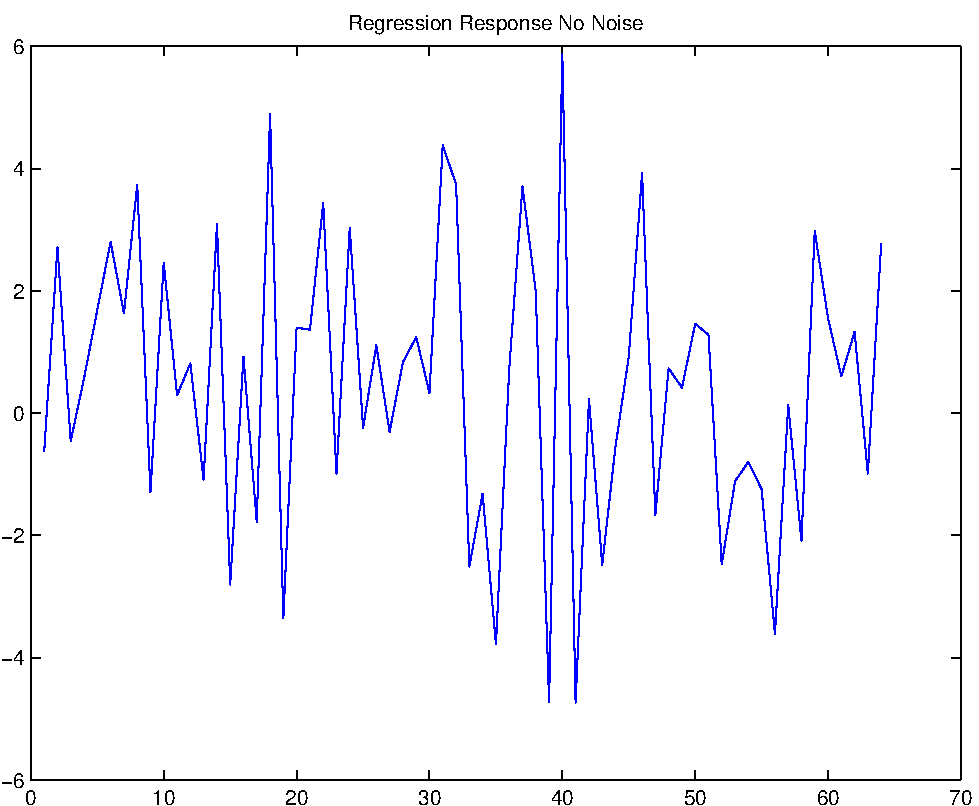
\includegraphics[width=10.0cm,height=10.0cm]{regression_response_no_noise.pdf}

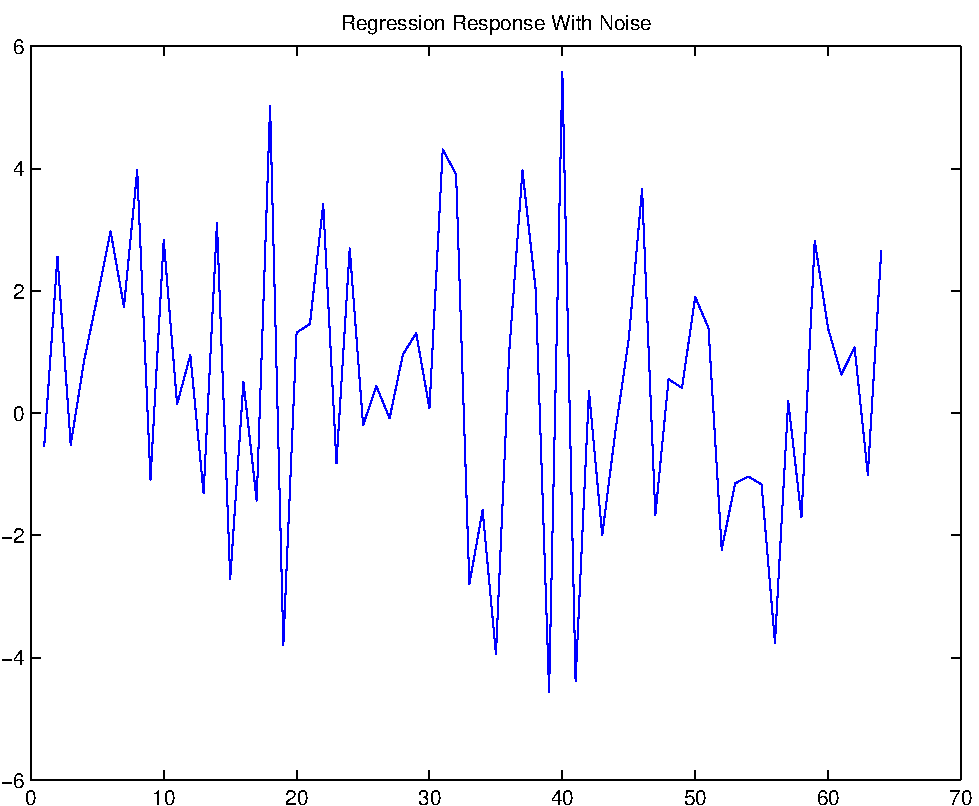
\includegraphics[width=10.0cm,height=10.0cm]{regression_response_with_noise.pdf}

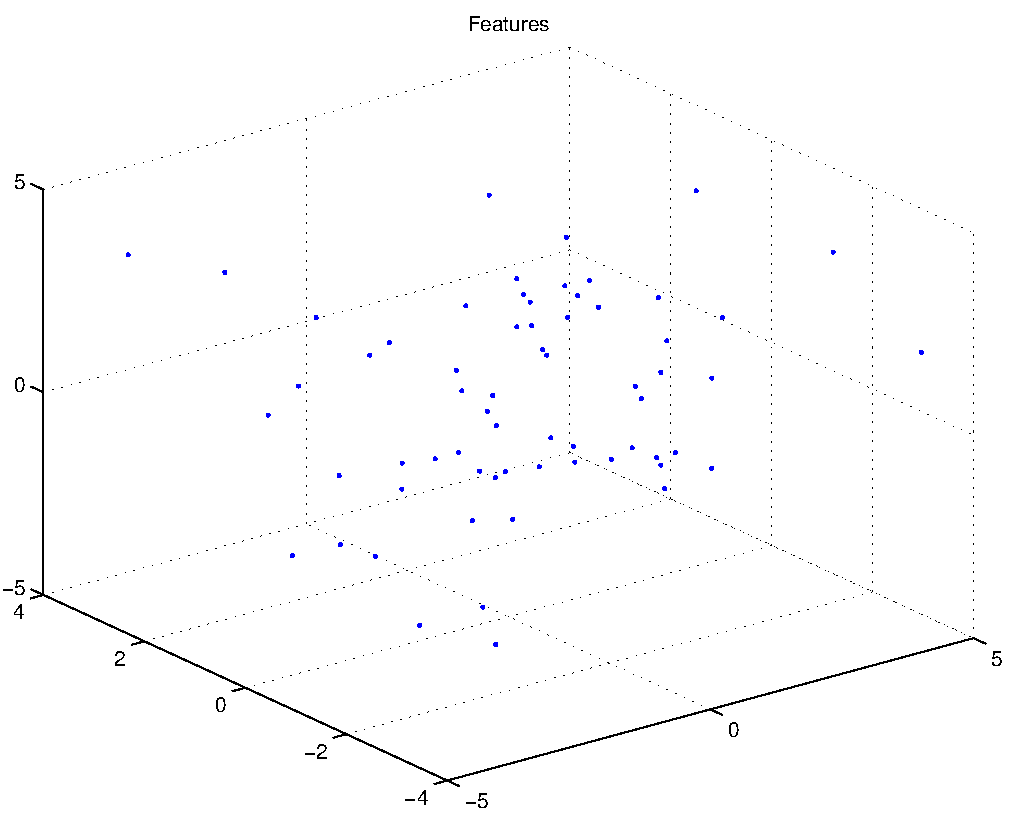
\includegraphics[width=10.0cm,height=10.0cm]{regression_features.pdf}

Beta
+0.817, +0.999, +0.510

Response
-0.543
+2.562
-0.519
+0.856
+1.900
+2.974
+1.739
+3.973
-1.090
+2.837
+0.145
+0.950
-1.311
+3.109
-2.714
+0.511
-1.432
+5.030
-3.794
+1.318
+1.459
+3.417
-0.823
+2.694
-0.198
+0.441
-0.085
+0.963
+1.308
+0.076
+4.313
+3.907
-2.798
-1.589
-3.946
+0.997
+3.971
+2.016
-4.562
+5.578
-4.384
+0.361
-1.996
-0.288
+1.205
+3.670
-1.668
+0.555
+0.413
+1.900
+1.397
-2.234
-1.151
-1.039
-1.167
-3.762
+0.196
-1.706
+2.822
+1.385
+0.631
+1.074
-1.007
+2.652
Estimate for Beta
+0.792
+0.982
+0.527
Error:
-0.025, -0.017, +0.016


QueryPerformanceCounter  =  +2.912
\subsubsection{Fast Gauss Transform}
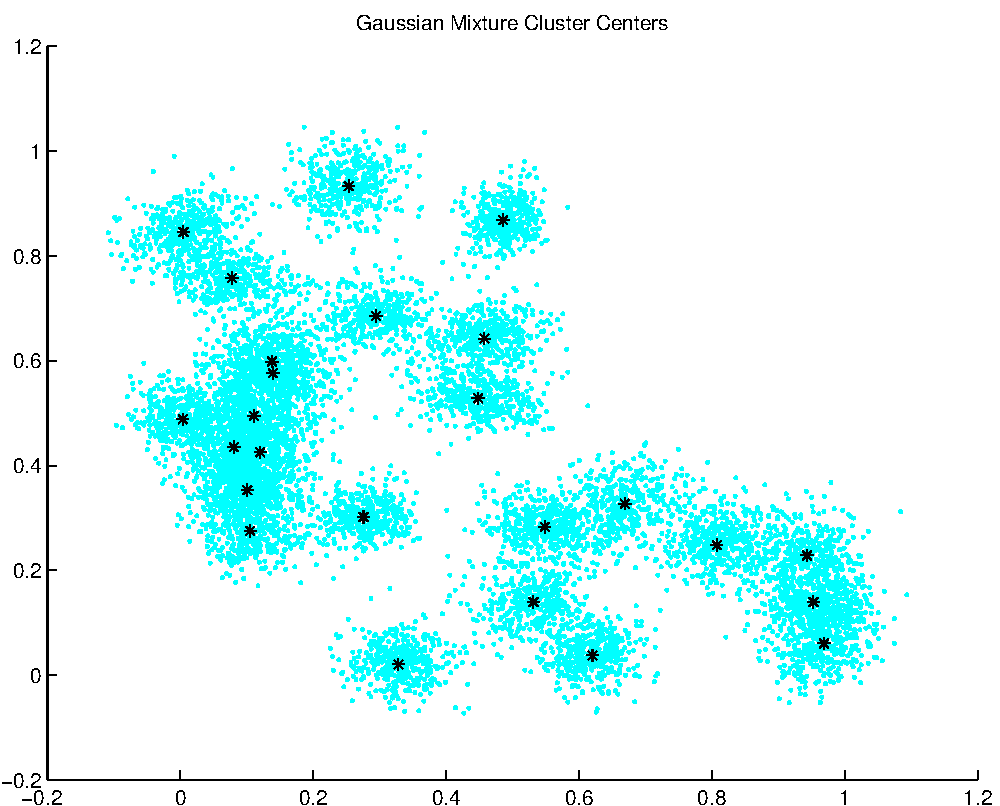
\includegraphics[width=10.0cm,height=10.0cm]{GaussianMixture_ClusterCenters25_Centers.pdf}

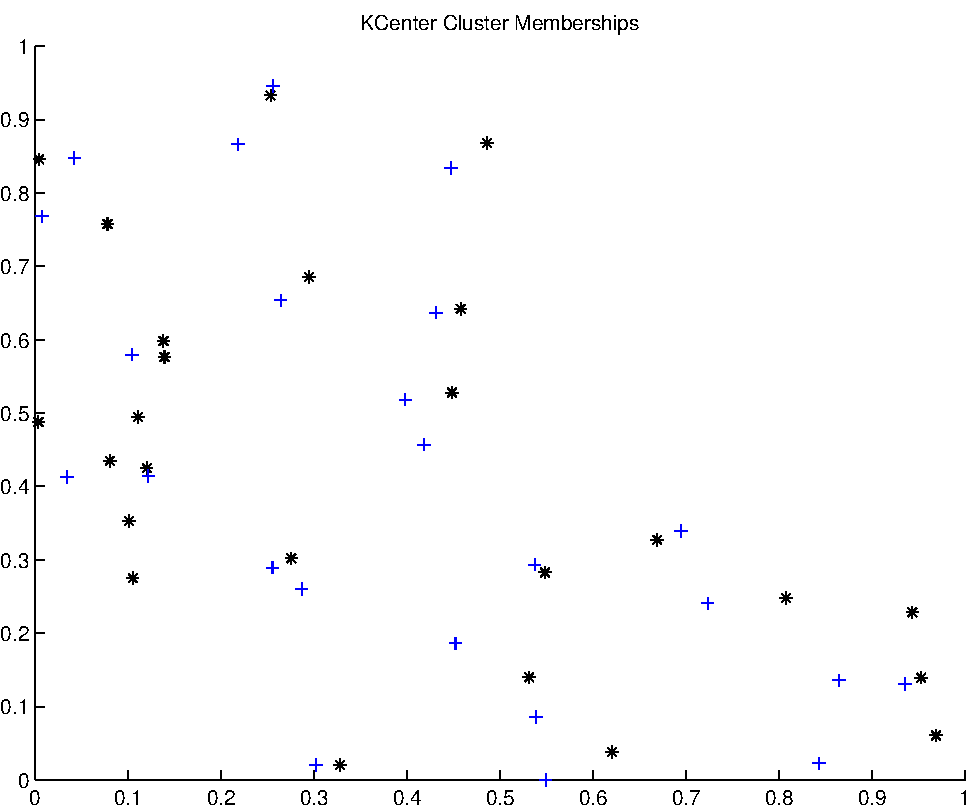
\includegraphics[width=10.0cm,height=10.0cm]{KCenterClusterMemberships_25_Centers.pdf}

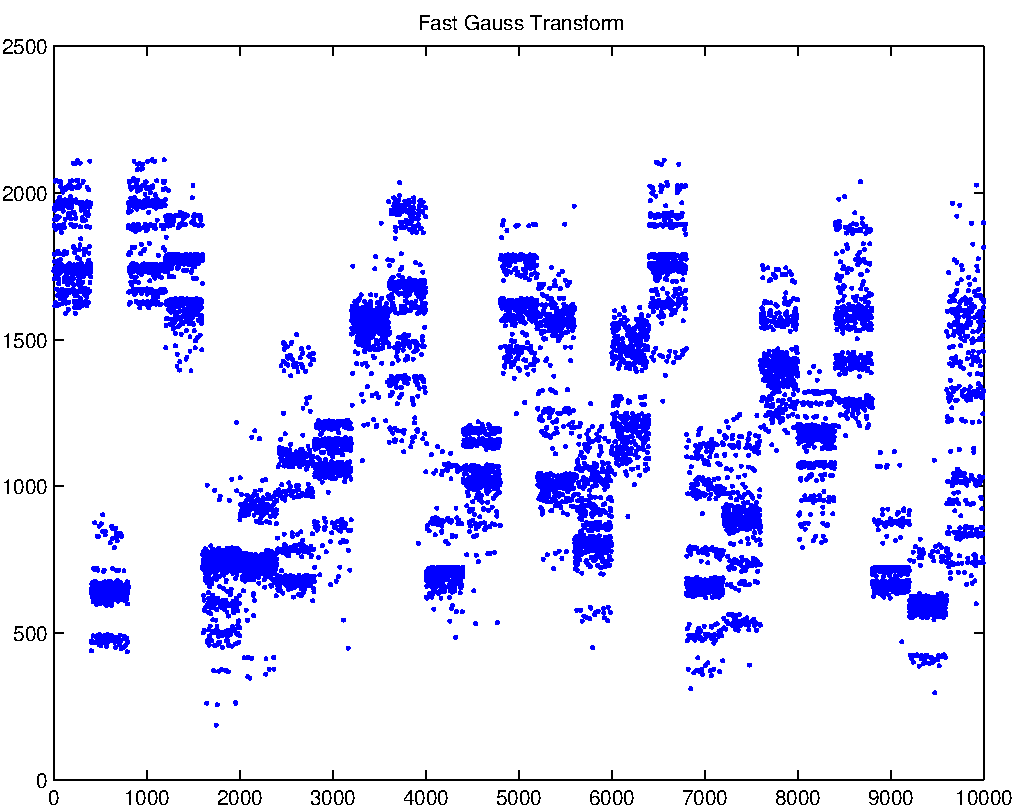
\includegraphics[width=10.0cm,height=10.0cm]{FGT25_Centers.pdf}

QueryPerformanceCounter  =  +7.179
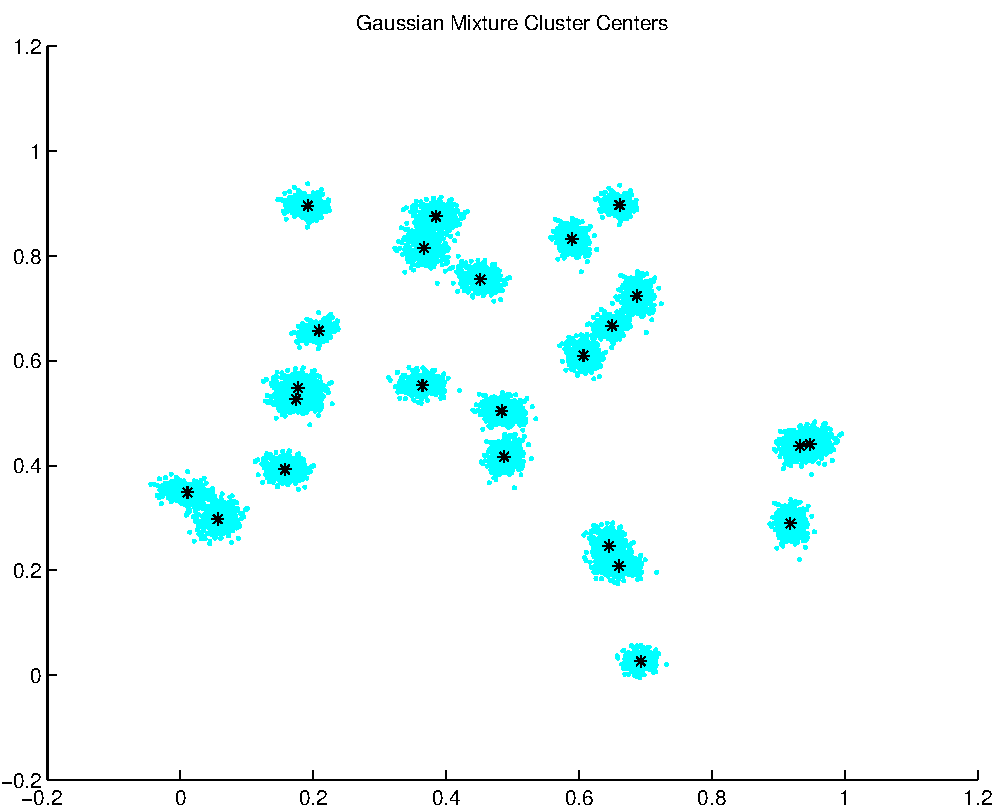
\includegraphics[width=10.0cm,height=10.0cm]{GaussianMixture_ClusterCenters24_Centers.pdf}

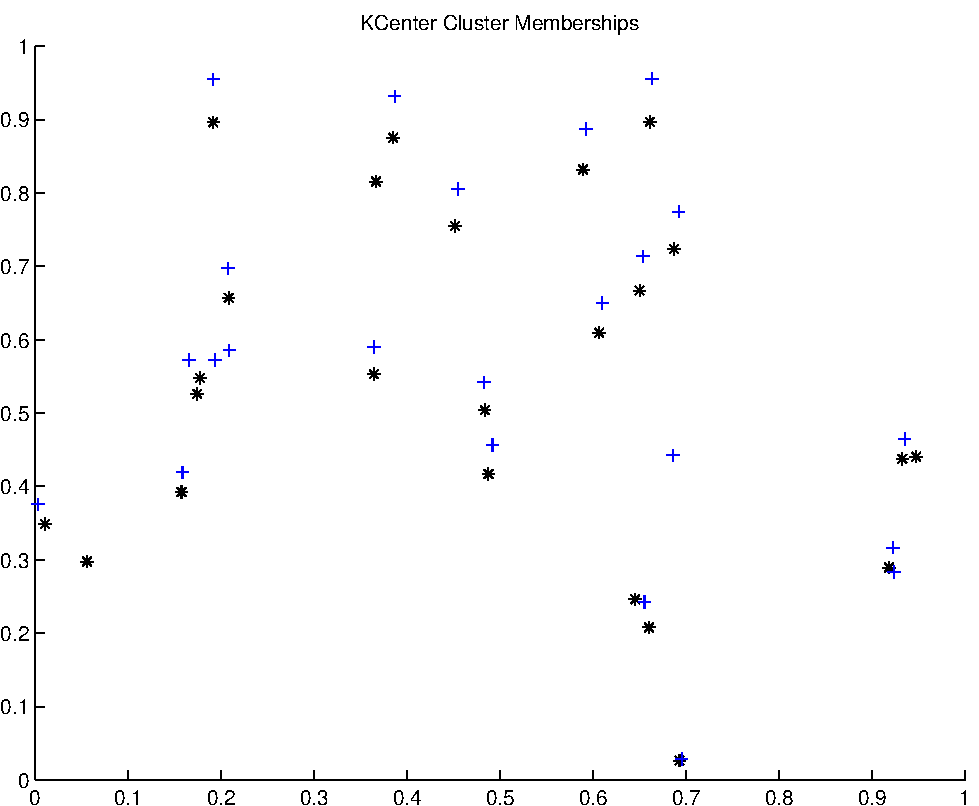
\includegraphics[width=10.0cm,height=10.0cm]{KCenterClusterMemberships_24_Centers.pdf}

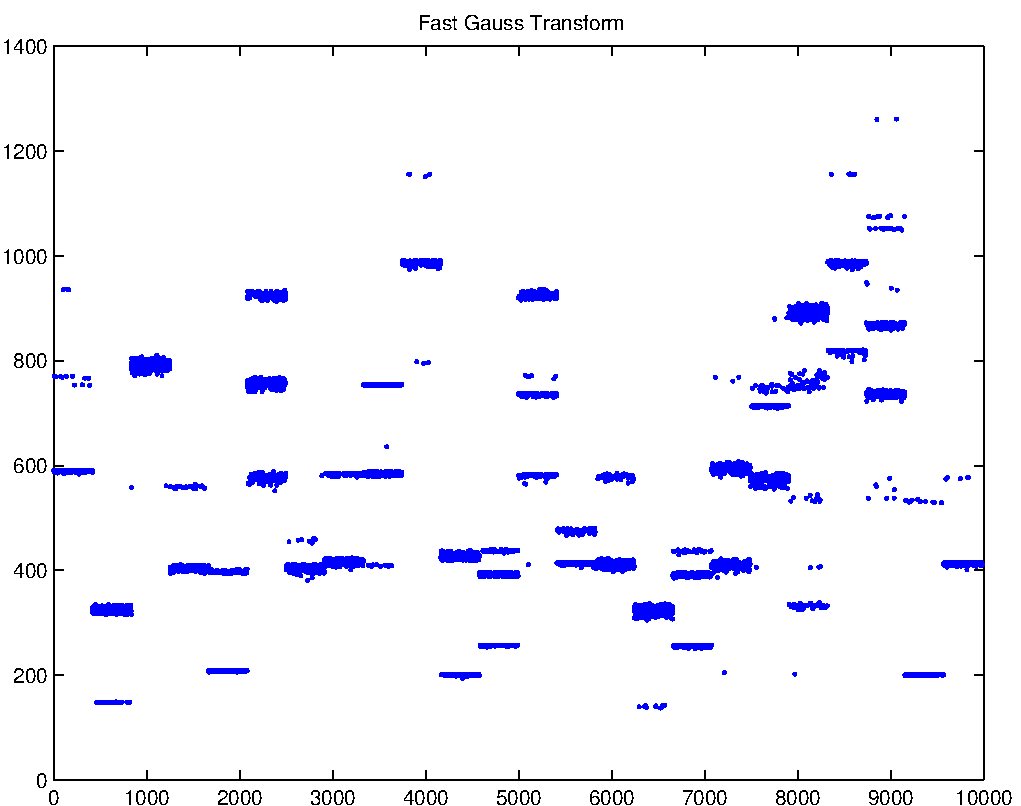
\includegraphics[width=10.0cm,height=10.0cm]{FGT24_Centers.pdf}

QueryPerformanceCounter  =  +6.129
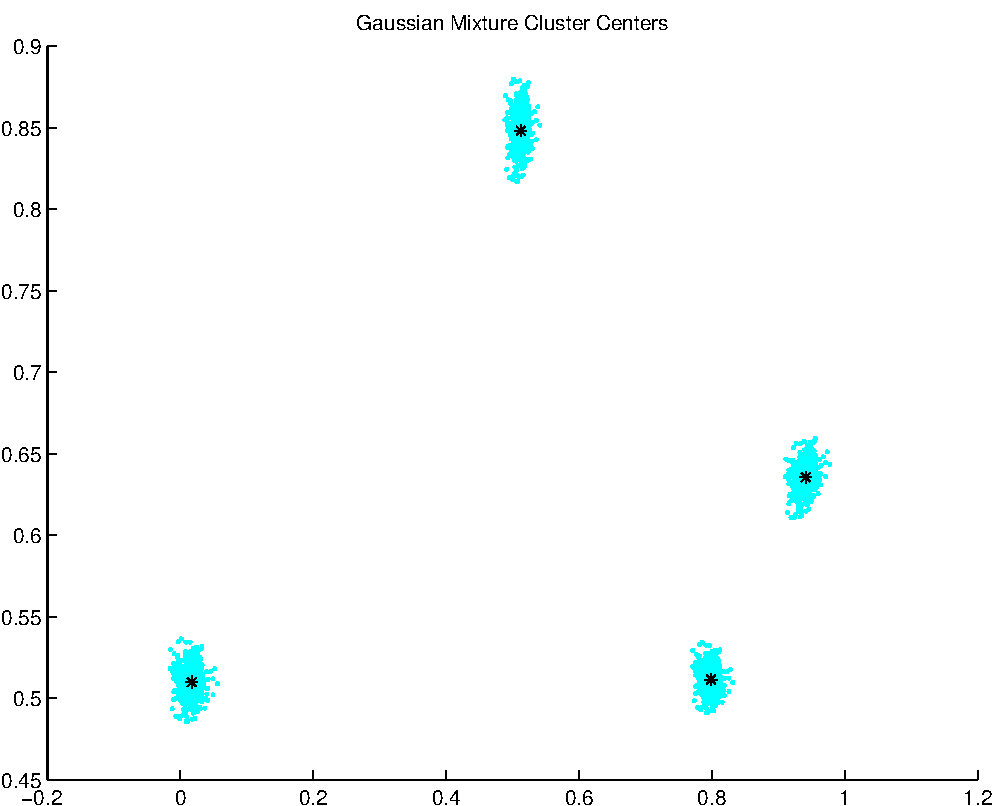
\includegraphics[width=10.0cm,height=10.0cm]{GaussianMixture_ClusterCenters4_Centers.pdf}

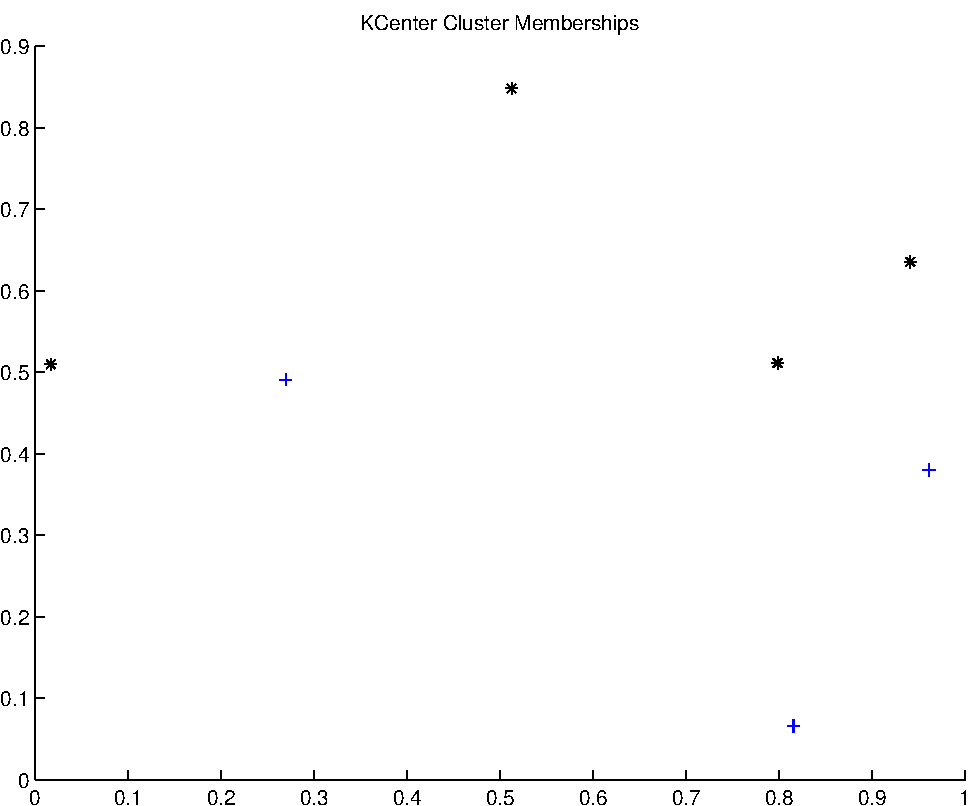
\includegraphics[width=10.0cm,height=10.0cm]{KCenterClusterMemberships_4_Centers.pdf}

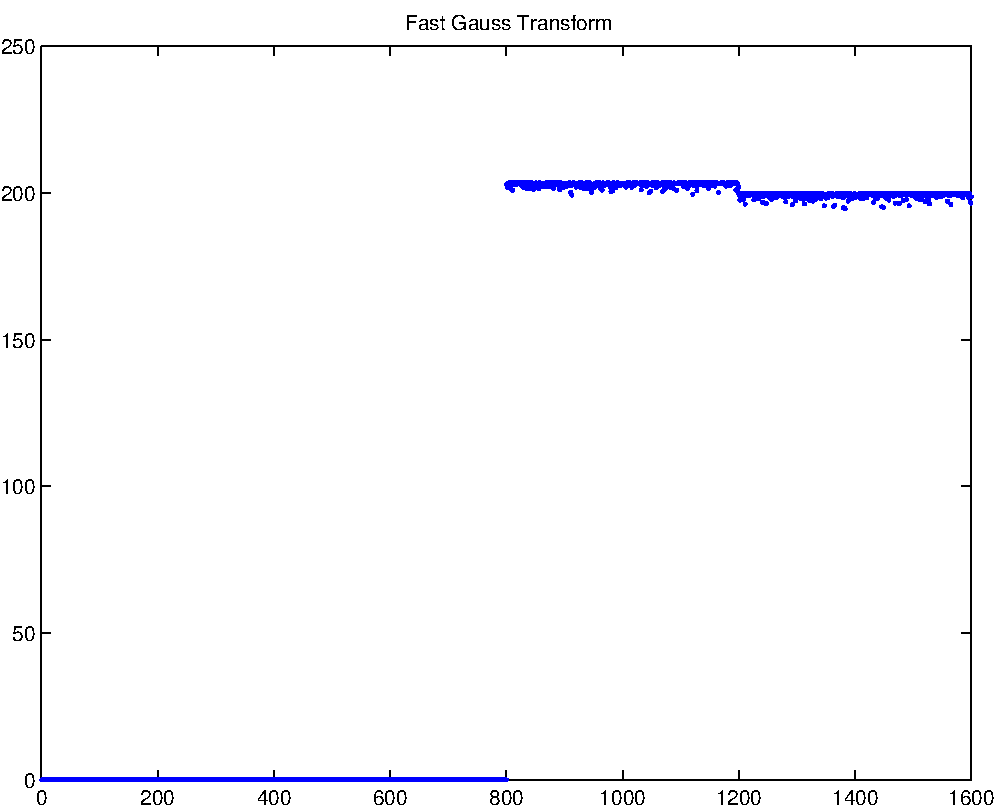
\includegraphics[width=10.0cm,height=10.0cm]{FGT4_Centers.pdf}

QueryPerformanceCounter  =  +3.791
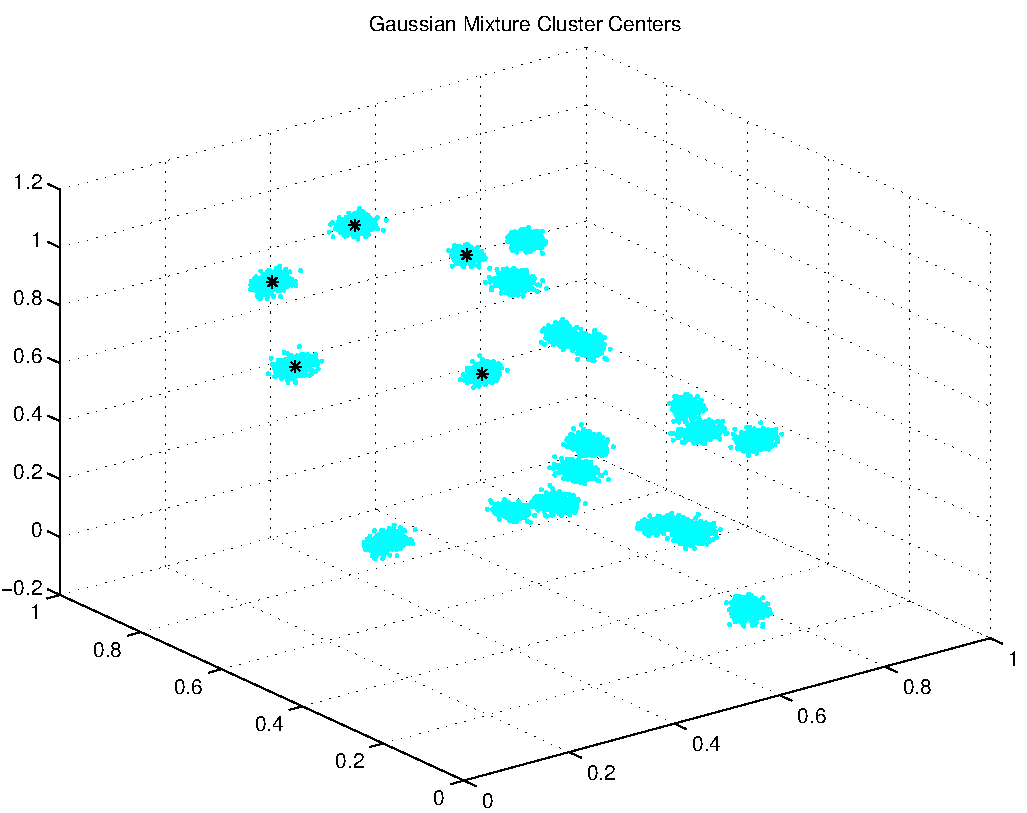
\includegraphics[width=10.0cm,height=10.0cm]{GaussianMixture_ClusterCenters20_Centers.pdf}

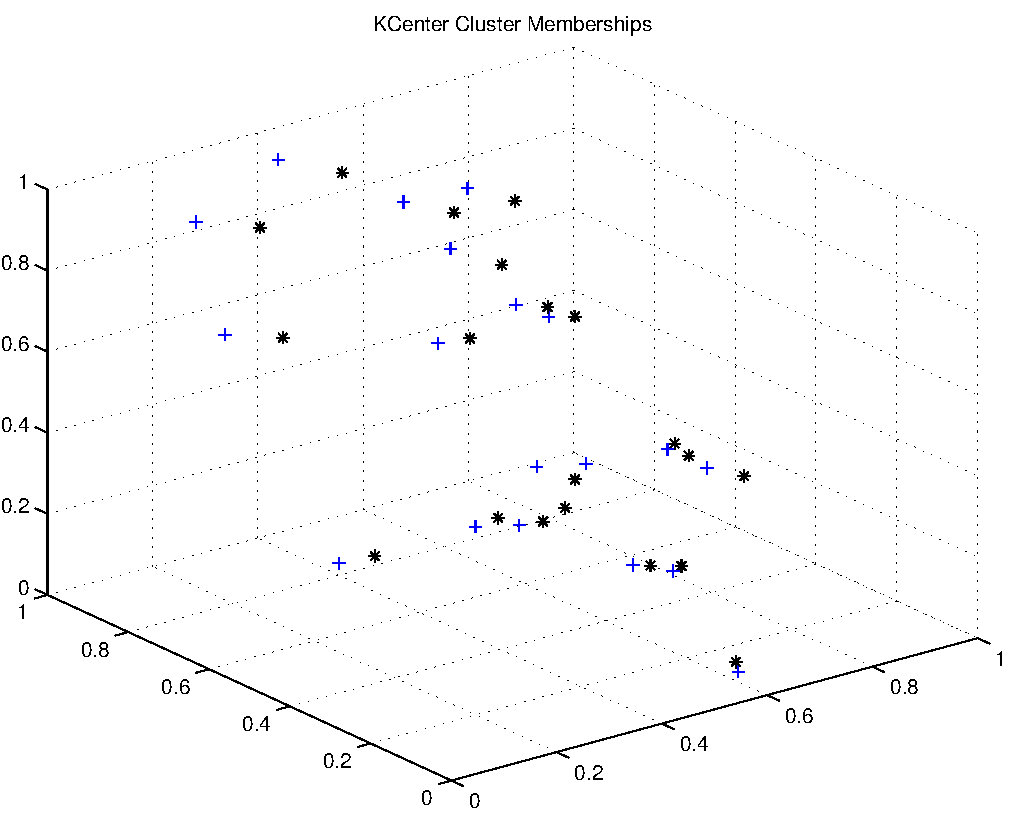
\includegraphics[width=10.0cm,height=10.0cm]{KCenterClusterMemberships_20_Centers.pdf}

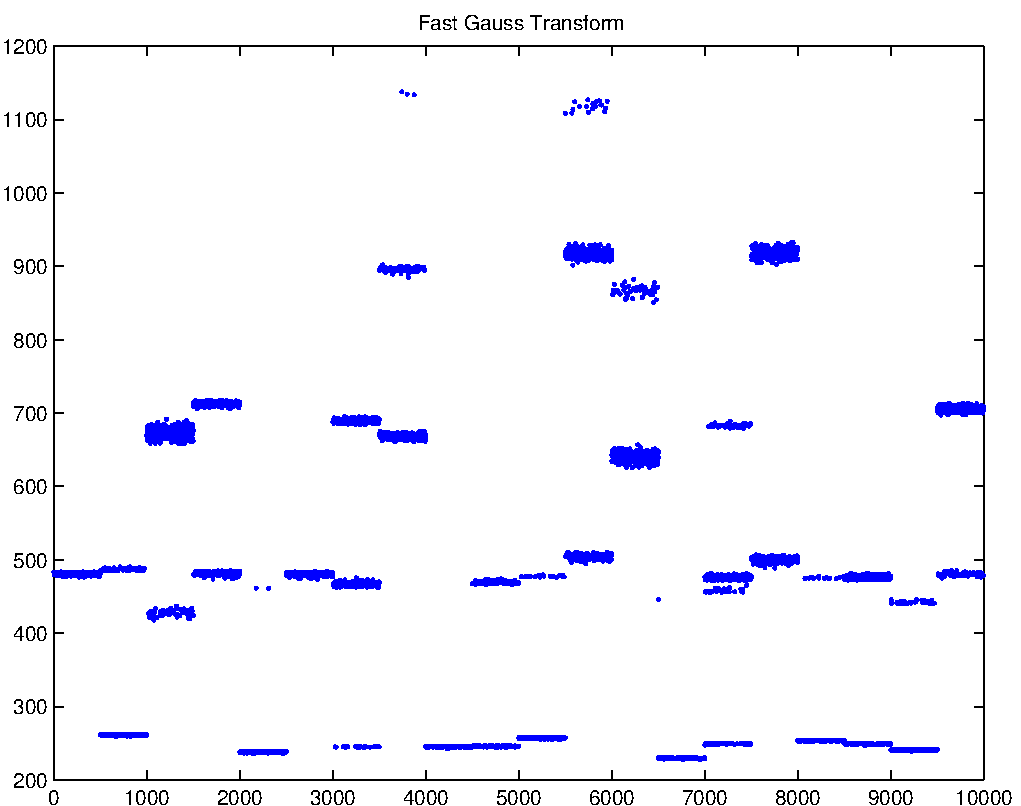
\includegraphics[width=10.0cm,height=10.0cm]{FGT20_Centers.pdf}

QueryPerformanceCounter  =  +6.267
\subsubsection{Matrix Norms}
\subsubsection{Haar Distributed Random Orthogonal Matrix $A \in O(n)$}
 Testing Operator Norm
Number of Dimensions: +12

$A = \left(
\begin{array}{
cccccccccccc}
+0.022 & +0.272 & +0.059 & +0.404 & +0.317 & -0.016 & +0.225 & -0.102 & +0.189 & -0.392 & -0.133 & +0.625 \\
+0.309 & +0.149 & -0.181 & +0.268 & -0.140 & -0.004 & -0.804 & -0.031 & +0.270 & -0.180 & +0.029 & -0.065 \\
-0.280 & +0.234 & -0.080 & -0.083 & +0.223 & +0.256 & +0.058 & +0.330 & +0.018 & -0.597 & +0.307 & -0.419 \\
+0.219 & -0.342 & +0.053 & -0.234 & +0.431 & -0.392 & -0.091 & -0.002 & +0.109 & -0.027 & +0.622 & +0.174 \\
-0.368 & -0.270 & -0.192 & +0.523 & +0.125 & -0.199 & -0.198 & +0.034 & -0.618 & -0.014 & +0.059 & +0.009 \\
+0.000 & -0.088 & +0.060 & -0.352 & -0.011 & +0.472 & -0.309 & +0.401 & -0.306 & -0.003 & -0.022 & +0.540 \\
-0.295 & -0.465 & -0.149 & +0.241 & +0.231 & +0.468 & -0.011 & +0.006 & +0.523 & +0.267 & +0.010 & -0.019 \\
-0.420 & +0.335 & +0.435 & -0.141 & +0.237 & +0.124 & -0.320 & -0.526 & -0.061 & +0.180 & +0.128 & -0.010 \\
+0.031 & +0.471 & -0.360 & +0.188 & -0.163 & +0.148 & +0.166 & +0.075 & -0.038 & +0.435 & +0.563 & +0.150 \\
-0.327 & +0.287 & -0.148 & -0.154 & +0.278 & -0.449 & -0.158 & +0.478 & +0.227 & +0.294 & -0.305 & +0.033 \\
+0.521 & +0.136 & +0.140 & +0.184 & +0.587 & +0.234 & +0.024 & +0.125 & -0.241 & +0.263 & -0.173 & -0.289 \\
+0.030 & +0.028 & -0.729 & -0.368 & +0.264 & +0.076 & -0.003 & -0.437 & -0.125 & -0.091 & -0.199 & +0.028 \\
\end{array}
\right)$ \newline 

$Det(A) :   A \in O(n)$ = (+1.000,-0.000)

$L = \left(
\begin{array}{
cccccccccccc}
+1.000 & +0.000 & +0.000 & +0.000 & +0.000 & +0.000 & +0.000 & +0.000 & +0.000 & +0.000 & +0.000 & +0.000 \\
+0.060 & +1.000 & +0.000 & +0.000 & +0.000 & +0.000 & +0.000 & +0.000 & +0.000 & +0.000 & +0.000 & +0.000 \\
-0.805 & +0.960 & +1.000 & +0.000 & +0.000 & +0.000 & +0.000 & +0.000 & +0.000 & +0.000 & +0.000 & +0.000 \\
-0.706 & -0.375 & -0.256 & +1.000 & +0.000 & +0.000 & +0.000 & +0.000 & +0.000 & +0.000 & +0.000 & +0.000 \\
+0.057 & +0.043 & -0.800 & -0.762 & +1.000 & +0.000 & +0.000 & +0.000 & +0.000 & +0.000 & +0.000 & +0.000 \\
-0.566 & -0.837 & -0.419 & +0.626 & +0.227 & +1.000 & +0.000 & +0.000 & +0.000 & +0.000 & +0.000 & +0.000 \\
+0.592 & +0.147 & -0.232 & +0.141 & -0.233 & -0.101 & +1.000 & +0.000 & +0.000 & +0.000 & +0.000 & +0.000 \\
-0.627 & +0.806 & +0.263 & -0.205 & +0.478 & -0.818 & -0.241 & +1.000 & +0.000 & +0.000 & +0.000 & +0.000 \\
+0.001 & -0.190 & -0.012 & -0.474 & +0.195 & +0.694 & +0.431 & +0.680 & +1.000 & +0.000 & +0.000 & +0.000 \\
-0.537 & +0.663 & +0.266 & -0.085 & +0.329 & +0.242 & -0.189 & +0.645 & +0.365 & +1.000 & +0.000 & +0.000 \\
+0.421 & -0.863 & -0.360 & -0.321 & +0.376 & -0.553 & -0.131 & +0.143 & -0.261 & -0.330 & +1.000 & +0.000 \\
+0.042 & +0.575 & +0.294 & +0.505 & -0.141 & -0.221 & -0.346 & -0.247 & -0.546 & +0.762 & -0.278 & +1.000 \\
\end{array}
\right)$ \newline 

$U = \left(
\begin{array}{
cccccccccccc}
+0.521 & +0.136 & +0.140 & +0.184 & +0.587 & +0.234 & +0.024 & +0.125 & -0.241 & +0.263 & -0.173 & -0.289 \\
+0.000 & +0.463 & -0.368 & +0.177 & -0.198 & +0.134 & +0.164 & +0.067 & -0.023 & +0.420 & +0.574 & +0.167 \\
+0.000 & +0.000 & +0.902 & -0.163 & +0.901 & +0.184 & -0.459 & -0.489 & -0.233 & -0.011 & -0.562 & -0.403 \\
+0.000 & +0.000 & +0.000 & +0.677 & +0.697 & +0.064 & -0.237 & +0.022 & -0.856 & +0.326 & +0.008 & -0.235 \\
+0.000 & +0.000 & +0.000 & +0.000 & +1.491 & +0.252 & -0.559 & -0.822 & -0.949 & +0.115 & -0.657 & -0.464 \\
+0.000 & +0.000 & +0.000 & +0.000 & +0.000 & +0.692 & +0.224 & +0.101 & +1.021 & +0.532 & +0.301 & +0.042 \\
+0.000 & +0.000 & +0.000 & +0.000 & +0.000 & +0.000 & -1.024 & -0.414 & +0.364 & -0.366 & -0.208 & -0.083 \\
+0.000 & +0.000 & +0.000 & +0.000 & +0.000 & +0.000 & +0.000 & +1.011 & +1.357 & +0.482 & -0.216 & +0.011 \\
+0.000 & +0.000 & +0.000 & +0.000 & +0.000 & +0.000 & +0.000 & +0.000 & -2.322 & -0.331 & +0.240 & +0.545 \\
+0.000 & +0.000 & +0.000 & +0.000 & +0.000 & +0.000 & +0.000 & +0.000 & +0.000 & -1.129 & +0.140 & -0.677 \\
+0.000 & +0.000 & +0.000 & +0.000 & +0.000 & +0.000 & +0.000 & +0.000 & +0.000 & +0.000 & +1.517 & +0.324 \\
+0.000 & +0.000 & +0.000 & +0.000 & +0.000 & +0.000 & +0.000 & +0.000 & +0.000 & +0.000 & +0.000 & +1.599 \\
\end{array}
\right)$ \newline 

$L * U  = \left(
\begin{array}{
cccccccccccc}
+0.521 & +0.136 & +0.140 & +0.184 & +0.587 & +0.234 & +0.024 & +0.125 & -0.241 & +0.263 & -0.173 & -0.289 \\
+0.031 & +0.471 & -0.360 & +0.188 & -0.163 & +0.148 & +0.166 & +0.075 & -0.038 & +0.435 & +0.563 & +0.150 \\
-0.420 & +0.335 & +0.435 & -0.141 & +0.237 & +0.124 & -0.320 & -0.526 & -0.061 & +0.180 & +0.128 & -0.010 \\
-0.368 & -0.270 & -0.192 & +0.523 & +0.125 & -0.199 & -0.198 & +0.034 & -0.618 & -0.014 & +0.059 & +0.009 \\
+0.030 & +0.028 & -0.729 & -0.368 & +0.264 & +0.076 & -0.003 & -0.437 & -0.125 & -0.091 & -0.199 & +0.028 \\
-0.295 & -0.465 & -0.149 & +0.241 & +0.231 & +0.468 & -0.011 & +0.006 & +0.523 & +0.267 & +0.010 & -0.019 \\
+0.309 & +0.149 & -0.181 & +0.268 & -0.140 & -0.004 & -0.804 & -0.031 & +0.270 & -0.180 & +0.029 & -0.065 \\
-0.327 & +0.287 & -0.148 & -0.154 & +0.278 & -0.449 & -0.158 & +0.478 & +0.227 & +0.294 & -0.305 & +0.033 \\
+0.000 & -0.088 & +0.060 & -0.352 & -0.011 & +0.472 & -0.309 & +0.401 & -0.306 & -0.003 & -0.022 & +0.540 \\
-0.280 & +0.234 & -0.080 & -0.083 & +0.223 & +0.256 & +0.058 & +0.330 & +0.018 & -0.597 & +0.307 & -0.419 \\
+0.219 & -0.342 & +0.053 & -0.234 & +0.431 & -0.392 & -0.091 & -0.002 & +0.109 & -0.027 & +0.622 & +0.174 \\
+0.022 & +0.272 & +0.059 & +0.404 & +0.317 & -0.016 & +0.225 & -0.102 & +0.189 & -0.392 & -0.133 & +0.625 \\
\end{array}
\right)$ \newline 

$Det(L) :    = (+1.000,+0.000)     Det(U) :    = (-1.000,+0.000)     Det(LU) :    = (-1.000,-0.000)$

$||A||_{L_1}$  = +3.139

$||A||_{L_{\infty}}$ = +3.139

$||A^{-1}||_{L_1}$  = +3.139

$||A^{-1}||_{L_{\infty}}$ = +3.139

$||A||_{L_{\infty}} * ||A^{-1}||_{L_{\infty}} = +9.852$

$||A||_{L_1} * ||A^{-1}||_{L_1} = +9.852$

Frobenious Norm  $||A||_{\textit{F}}$ via $\sum\limits_{i,j =0}^{n} \|A_{i,j}|$   of  $A \in O(n)$  +3.464

$L_1$ condition number of Haar Distributed Random Orthogonal Matrix $A \in O(n)$ +8.749

$A = \left(
\begin{array}{
cccccccccccc}
+0.022 & +0.272 & +0.059 & +0.404 & +0.317 & -0.016 & +0.225 & -0.102 & +0.189 & -0.392 & -0.133 & +0.625 \\
+0.309 & +0.149 & -0.181 & +0.268 & -0.140 & -0.004 & -0.804 & -0.031 & +0.270 & -0.180 & +0.029 & -0.065 \\
-0.280 & +0.234 & -0.080 & -0.083 & +0.223 & +0.256 & +0.058 & +0.330 & +0.018 & -0.597 & +0.307 & -0.419 \\
+0.219 & -0.342 & +0.053 & -0.234 & +0.431 & -0.392 & -0.091 & -0.002 & +0.109 & -0.027 & +0.622 & +0.174 \\
-0.368 & -0.270 & -0.192 & +0.523 & +0.125 & -0.199 & -0.198 & +0.034 & -0.618 & -0.014 & +0.059 & +0.009 \\
+0.000 & -0.088 & +0.060 & -0.352 & -0.011 & +0.472 & -0.309 & +0.401 & -0.306 & -0.003 & -0.022 & +0.540 \\
-0.295 & -0.465 & -0.149 & +0.241 & +0.231 & +0.468 & -0.011 & +0.006 & +0.523 & +0.267 & +0.010 & -0.019 \\
-0.420 & +0.335 & +0.435 & -0.141 & +0.237 & +0.124 & -0.320 & -0.526 & -0.061 & +0.180 & +0.128 & -0.010 \\
+0.031 & +0.471 & -0.360 & +0.188 & -0.163 & +0.148 & +0.166 & +0.075 & -0.038 & +0.435 & +0.563 & +0.150 \\
-0.327 & +0.287 & -0.148 & -0.154 & +0.278 & -0.449 & -0.158 & +0.478 & +0.227 & +0.294 & -0.305 & +0.033 \\
+0.521 & +0.136 & +0.140 & +0.184 & +0.587 & +0.234 & +0.024 & +0.125 & -0.241 & +0.263 & -0.173 & -0.289 \\
+0.030 & +0.028 & -0.729 & -0.368 & +0.264 & +0.076 & -0.003 & -0.437 & -0.125 & -0.091 & -0.199 & +0.028 \\
\end{array}
\right)$ \newline 

$L_{\infty}$ condition number of Haar Distributed Random Orthogonal Matrix $A \in O(n)$ +7.406

Eigenvalues of $A \in O(n)$

(+0.466,+0.885), (+0.466,-0.885), (-0.565,+0.825), (-0.565,-0.825), (-0.771,+0.636), (-0.771,-0.636), (-0.998,+0.068), (-0.998,-0.068), (+0.893,+0.451), (+0.893,-0.451), (+0.990,+0.139), (+0.990,-0.139)

 $|\lambda | : \lambda \in \sigma(A) , A \in O(n)$

+1.000, +1.000, +1.000, +1.000, +1.000, +1.000, +1.000, +1.000, +1.000, +1.000, +1.000, +1.000


Calculating $A^{\dag} A,$  we expect $A^{\dag} A \approx I$

$A^{\dag} A = \left(
\begin{array}{
cccccccccccc}
+1.000 & +0.000 & +0.000 & -0.000 & -0.000 & -0.000 & -0.000 & +0.000 & +0.000 & +0.000 & +0.000 & -0.000 \\
+0.000 & +1.000 & +0.000 & -0.000 & -0.000 & -0.000 & -0.000 & -0.000 & -0.000 & -0.000 & +0.000 & -0.000 \\
+0.000 & +0.000 & +1.000 & -0.000 & -0.000 & -0.000 & -0.000 & -0.000 & -0.000 & +0.000 & +0.000 & +0.000 \\
-0.000 & -0.000 & -0.000 & +1.000 & -0.000 & -0.000 & +0.000 & -0.000 & -0.000 & +0.000 & -0.000 & -0.000 \\
-0.000 & -0.000 & -0.000 & -0.000 & +1.000 & +0.000 & -0.000 & +0.000 & +0.000 & -0.000 & +0.000 & +0.000 \\
-0.000 & -0.000 & -0.000 & -0.000 & +0.000 & +1.000 & -0.000 & +0.000 & +0.000 & +0.000 & -0.000 & +0.000 \\
-0.000 & -0.000 & -0.000 & +0.000 & -0.000 & -0.000 & +1.000 & +0.000 & -0.000 & -0.000 & -0.000 & -0.000 \\
+0.000 & -0.000 & -0.000 & -0.000 & +0.000 & +0.000 & +0.000 & +1.000 & -0.000 & -0.000 & +0.000 & +0.000 \\
+0.000 & -0.000 & -0.000 & -0.000 & +0.000 & +0.000 & -0.000 & -0.000 & +1.000 & -0.000 & +0.000 & -0.000 \\
+0.000 & -0.000 & +0.000 & +0.000 & -0.000 & +0.000 & -0.000 & -0.000 & -0.000 & +1.000 & +0.000 & +0.000 \\
+0.000 & +0.000 & +0.000 & -0.000 & +0.000 & -0.000 & -0.000 & +0.000 & +0.000 & +0.000 & +1.000 & +0.000 \\
-0.000 & -0.000 & +0.000 & -0.000 & +0.000 & +0.000 & -0.000 & +0.000 & -0.000 & +0.000 & +0.000 & +1.000 \\
\end{array}
\right)$ \newline 

Calculating $A^{-1} ,  A \in O(n)$.

$A^{-1} = \left(
\begin{array}{
cccccccccccc}
+0.022 & +0.309 & -0.280 & +0.219 & -0.368 & +0.000 & -0.295 & -0.420 & +0.031 & -0.327 & +0.521 & +0.030 \\
+0.272 & +0.149 & +0.234 & -0.342 & -0.270 & -0.088 & -0.465 & +0.335 & +0.471 & +0.287 & +0.136 & +0.028 \\
+0.059 & -0.181 & -0.080 & +0.053 & -0.192 & +0.060 & -0.149 & +0.435 & -0.360 & -0.148 & +0.140 & -0.729 \\
+0.404 & +0.268 & -0.083 & -0.234 & +0.523 & -0.352 & +0.241 & -0.141 & +0.188 & -0.154 & +0.184 & -0.368 \\
+0.317 & -0.140 & +0.223 & +0.431 & +0.125 & -0.011 & +0.231 & +0.237 & -0.163 & +0.278 & +0.587 & +0.264 \\
-0.016 & -0.004 & +0.256 & -0.392 & -0.199 & +0.472 & +0.468 & +0.124 & +0.148 & -0.449 & +0.234 & +0.076 \\
+0.225 & -0.804 & +0.058 & -0.091 & -0.198 & -0.309 & -0.011 & -0.320 & +0.166 & -0.158 & +0.024 & -0.003 \\
-0.102 & -0.031 & +0.330 & -0.002 & +0.034 & +0.401 & +0.006 & -0.526 & +0.075 & +0.478 & +0.125 & -0.437 \\
+0.189 & +0.270 & +0.018 & +0.109 & -0.618 & -0.306 & +0.523 & -0.061 & -0.038 & +0.227 & -0.241 & -0.125 \\
-0.392 & -0.180 & -0.597 & -0.027 & -0.014 & -0.003 & +0.267 & +0.180 & +0.435 & +0.294 & +0.263 & -0.091 \\
-0.133 & +0.029 & +0.307 & +0.622 & +0.059 & -0.022 & +0.010 & +0.128 & +0.563 & -0.305 & -0.173 & -0.199 \\
+0.625 & -0.065 & -0.419 & +0.174 & +0.009 & +0.540 & -0.019 & -0.010 & +0.150 & +0.033 & -0.289 & +0.028 \\
\end{array}
\right)$ \newline 

Calculating $A^{-1} *A  ,  A \in O(n)$.   We expect $A^{-1} *A  \approx I$. 

$A^{-1} *A = \left(
\begin{array}{
cccccccccccc}
+1.000 & -0.000 & -0.000 & -0.000 & -0.000 & -0.000 & +0.000 & -0.000 & -0.000 & -0.000 & +0.000 & +0.000 \\
+0.000 & +1.000 & +0.000 & -0.000 & -0.000 & -0.000 & -0.000 & +0.000 & +0.000 & -0.000 & -0.000 & -0.000 \\
+0.000 & -0.000 & +1.000 & -0.000 & -0.000 & -0.000 & -0.000 & -0.000 & +0.000 & -0.000 & -0.000 & -0.000 \\
-0.000 & -0.000 & +0.000 & +1.000 & -0.000 & -0.000 & -0.000 & +0.000 & -0.000 & +0.000 & -0.000 & -0.000 \\
+0.000 & -0.000 & +0.000 & +0.000 & +1.000 & +0.000 & +0.000 & +0.000 & +0.000 & -0.000 & +0.000 & -0.000 \\
-0.000 & +0.000 & +0.000 & +0.000 & +0.000 & +1.000 & -0.000 & -0.000 & +0.000 & +0.000 & +0.000 & +0.000 \\
+0.000 & -0.000 & -0.000 & +0.000 & -0.000 & +0.000 & +1.000 & +0.000 & +0.000 & -0.000 & -0.000 & -0.000 \\
-0.000 & -0.000 & +0.000 & +0.000 & +0.000 & -0.000 & -0.000 & +1.000 & +0.000 & -0.000 & +0.000 & -0.000 \\
+0.000 & +0.000 & +0.000 & +0.000 & +0.000 & +0.000 & -0.000 & +0.000 & +1.000 & +0.000 & +0.000 & -0.000 \\
-0.000 & +0.000 & +0.000 & +0.000 & -0.000 & -0.000 & -0.000 & -0.000 & -0.000 & +1.000 & -0.000 & +0.000 \\
-0.000 & +0.000 & -0.000 & -0.000 & +0.000 & +0.000 & -0.000 & -0.000 & +0.000 & -0.000 & +1.000 & -0.000 \\
-0.000 & +0.000 & +0.000 & +0.000 & +0.000 & +0.000 & +0.000 & -0.000 & +0.000 & +0.000 & +0.000 & +1.000 \\
\end{array}
\right)$ \newline 

Calculating SVD of  $A \in O(n)$

$U = \left(
\begin{array}{
cccccccccccc}
+0.090 & +0.323 & +0.186 & -0.038 & +0.001 & -0.001 & +0.586 & +0.474 & -0.153 & -0.073 & +0.476 & -0.168 \\
-0.093 & +0.056 & -0.116 & +0.248 & +0.166 & -0.679 & +0.101 & -0.178 & -0.325 & -0.236 & -0.196 & -0.429 \\
+0.044 & -0.143 & -0.585 & +0.047 & +0.348 & +0.430 & +0.419 & -0.206 & -0.248 & +0.186 & -0.070 & -0.088 \\
-0.027 & +0.171 & -0.435 & -0.548 & +0.163 & -0.486 & +0.058 & +0.047 & +0.285 & +0.200 & +0.115 & +0.277 \\
+0.093 & -0.394 & +0.069 & -0.294 & +0.408 & -0.007 & -0.242 & +0.382 & -0.463 & -0.329 & -0.004 & +0.226 \\
-0.193 & +0.291 & -0.009 & +0.282 & -0.049 & -0.096 & -0.208 & +0.142 & -0.525 & +0.575 & +0.020 & +0.342 \\
-0.010 & +0.256 & -0.393 & +0.203 & +0.022 & +0.135 & -0.249 & +0.643 & +0.234 & -0.101 & -0.357 & -0.229 \\
-0.105 & +0.508 & +0.377 & -0.423 & +0.362 & +0.211 & -0.022 & -0.158 & -0.076 & +0.076 & -0.401 & -0.191 \\
-0.022 & -0.272 & -0.059 & -0.404 & -0.317 & +0.016 & -0.225 & +0.102 & -0.189 & +0.392 & +0.133 & -0.625 \\
+0.086 & +0.148 & -0.183 & -0.283 & -0.649 & +0.047 & +0.208 & -0.036 & -0.342 & -0.304 & -0.365 & +0.218 \\
+0.117 & +0.422 & -0.279 & -0.022 & +0.010 & +0.173 & -0.456 & -0.286 & -0.159 & -0.343 & +0.510 & -0.089 \\
+0.950 & +0.072 & +0.064 & +0.071 & +0.045 & -0.119 & -0.055 & -0.029 & -0.019 & +0.216 & -0.128 & -0.013 \\
\end{array}
\right)$ \newline 

$S = \left(
\begin{array}{
cccccccccccc}
+1.000 & +0.000 & +0.000 & +0.000 & +0.000 & +0.000 & +0.000 & +0.000 & +0.000 & +0.000 & +0.000 & +0.000 \\
+0.000 & +1.000 & +0.000 & +0.000 & +0.000 & +0.000 & +0.000 & +0.000 & +0.000 & +0.000 & +0.000 & +0.000 \\
+0.000 & +0.000 & +1.000 & +0.000 & +0.000 & +0.000 & +0.000 & +0.000 & +0.000 & +0.000 & +0.000 & +0.000 \\
+0.000 & +0.000 & +0.000 & +1.000 & +0.000 & +0.000 & +0.000 & +0.000 & +0.000 & +0.000 & +0.000 & +0.000 \\
+0.000 & +0.000 & +0.000 & +0.000 & +1.000 & +0.000 & +0.000 & +0.000 & +0.000 & +0.000 & +0.000 & +0.000 \\
+0.000 & +0.000 & +0.000 & +0.000 & +0.000 & +1.000 & +0.000 & +0.000 & +0.000 & +0.000 & +0.000 & +0.000 \\
+0.000 & +0.000 & +0.000 & +0.000 & +0.000 & +0.000 & +1.000 & +0.000 & +0.000 & +0.000 & +0.000 & +0.000 \\
+0.000 & +0.000 & +0.000 & +0.000 & +0.000 & +0.000 & +0.000 & +1.000 & +0.000 & +0.000 & +0.000 & +0.000 \\
+0.000 & +0.000 & +0.000 & +0.000 & +0.000 & +0.000 & +0.000 & +0.000 & +1.000 & +0.000 & +0.000 & +0.000 \\
+0.000 & +0.000 & +0.000 & +0.000 & +0.000 & +0.000 & +0.000 & +0.000 & +0.000 & +1.000 & +0.000 & +0.000 \\
+0.000 & +0.000 & +0.000 & +0.000 & +0.000 & +0.000 & +0.000 & +0.000 & +0.000 & +0.000 & +1.000 & +0.000 \\
+0.000 & +0.000 & +0.000 & +0.000 & +0.000 & +0.000 & +0.000 & +0.000 & +0.000 & +0.000 & +0.000 & +1.000 \\
\end{array}
\right)$ \newline 

$V = \left(
\begin{array}{
cccccccccccc}
-0.000 & -0.000 & +0.000 & -0.000 & +0.000 & -0.000 & -0.000 & -0.000 & -1.000 & +0.000 & -0.000 & -0.000 \\
-0.457 & -0.052 & -0.367 & -0.094 & -0.076 & -0.035 & +0.422 & -0.200 & -0.000 & -0.132 & +0.556 & +0.304 \\
+0.487 & +0.092 & +0.041 & -0.137 & +0.194 & -0.391 & +0.365 & +0.144 & +0.000 & -0.112 & +0.411 & -0.456 \\
+0.127 & -0.000 & -0.130 & +0.441 & +0.423 & -0.175 & -0.414 & -0.295 & -0.000 & -0.510 & +0.144 & +0.152 \\
-0.153 & +0.489 & +0.173 & -0.303 & +0.311 & +0.521 & -0.003 & -0.369 & +0.000 & -0.121 & +0.065 & -0.304 \\
-0.049 & -0.651 & -0.022 & -0.019 & +0.628 & +0.294 & +0.094 & +0.095 & +0.000 & +0.257 & +0.052 & -0.078 \\
-0.308 & -0.430 & +0.348 & -0.131 & -0.163 & -0.190 & +0.162 & -0.201 & +0.000 & -0.533 & -0.276 & -0.304 \\
-0.221 & -0.054 & -0.177 & -0.078 & -0.160 & +0.238 & -0.422 & +0.609 & +0.000 & -0.305 & +0.309 & -0.304 \\
+0.430 & -0.277 & +0.252 & +0.231 & -0.436 & +0.490 & +0.035 & -0.241 & +0.000 & -0.063 & +0.356 & +0.038 \\
-0.030 & +0.178 & -0.220 & +0.582 & +0.036 & +0.289 & +0.522 & +0.245 & +0.000 & -0.215 & -0.307 & -0.152 \\
+0.167 & +0.081 & +0.366 & -0.279 & +0.191 & +0.127 & +0.176 & +0.394 & +0.000 & -0.380 & -0.040 & +0.608 \\
-0.393 & +0.151 & +0.646 & +0.440 & +0.086 & -0.157 & -0.001 & +0.149 & +0.000 & +0.240 & +0.316 & -0.019 \\
\end{array}
\right)$ \newline 

$U S V = \left(
\begin{array}{
cccccccccccc}
-0.265 & -0.233 & +0.057 & -0.471 & -0.036 & -0.085 & +0.156 & +0.326 & -0.090 & -0.697 & +0.131 & -0.017 \\
-0.031 & +0.443 & -0.326 & -0.263 & -0.225 & -0.359 & -0.262 & -0.476 & +0.093 & -0.273 & -0.259 & +0.046 \\
-0.461 & -0.242 & +0.070 & -0.006 & +0.354 & +0.342 & -0.023 & -0.302 & -0.044 & -0.050 & -0.618 & -0.052 \\
-0.362 & +0.327 & +0.291 & +0.022 & -0.672 & +0.371 & +0.218 & +0.043 & +0.027 & +0.078 & -0.056 & +0.168 \\
-0.175 & +0.418 & +0.205 & -0.421 & +0.228 & +0.028 & -0.410 & +0.369 & -0.093 & +0.311 & -0.015 & -0.336 \\
-0.431 & +0.405 & -0.279 & +0.489 & +0.313 & -0.179 & +0.185 & +0.321 & +0.193 & -0.148 & +0.035 & +0.077 \\
-0.224 & -0.201 & -0.534 & +0.086 & -0.174 & +0.437 & -0.525 & +0.022 & +0.010 & -0.037 & +0.342 & -0.038 \\
-0.154 & +0.040 & -0.344 & -0.329 & +0.072 & +0.090 & +0.576 & -0.278 & +0.105 & +0.271 & +0.274 & -0.408 \\
+0.314 & -0.027 & -0.491 & -0.156 & -0.162 & +0.145 & +0.176 & +0.492 & +0.022 & +0.106 & -0.550 & +0.042 \\
-0.436 & -0.416 & -0.072 & -0.001 & -0.280 & -0.592 & -0.067 & +0.105 & -0.086 & +0.414 & -0.087 & +0.034 \\
-0.075 & +0.067 & -0.109 & -0.353 & +0.283 & +0.074 & +0.054 & -0.046 & -0.117 & +0.229 & +0.165 & +0.818 \\
-0.001 & +0.158 & -0.144 & +0.165 & -0.020 & -0.009 & +0.106 & -0.056 & -0.950 & -0.050 & +0.007 & -0.087 \\
\end{array}
\right)$ \newline 

\subsubsection{Wishart Matrix $A \in W(n)$}
$L_1$ condition number of Wishart Matrix +56267.800
$L_infty$ condition number of Wishart Matrix +56267.800
\subsubsection{Gaussian Orthogonal Ensemble $A \in GOE(n)$}
$L_1$ condition number of GOE Matrix +470.231
$L_\infty$ condition number of GOE Matrix +470.231
\subsubsection{The Identity Matrix $I \in M(n)$}
$L_1$ condition number of $I$ = +1.000
$L_\infty$ condition number of $I$ = +1.000
QueryPerformanceCounter  =  +0.345
\subsubsection{Principal Components Matlab }
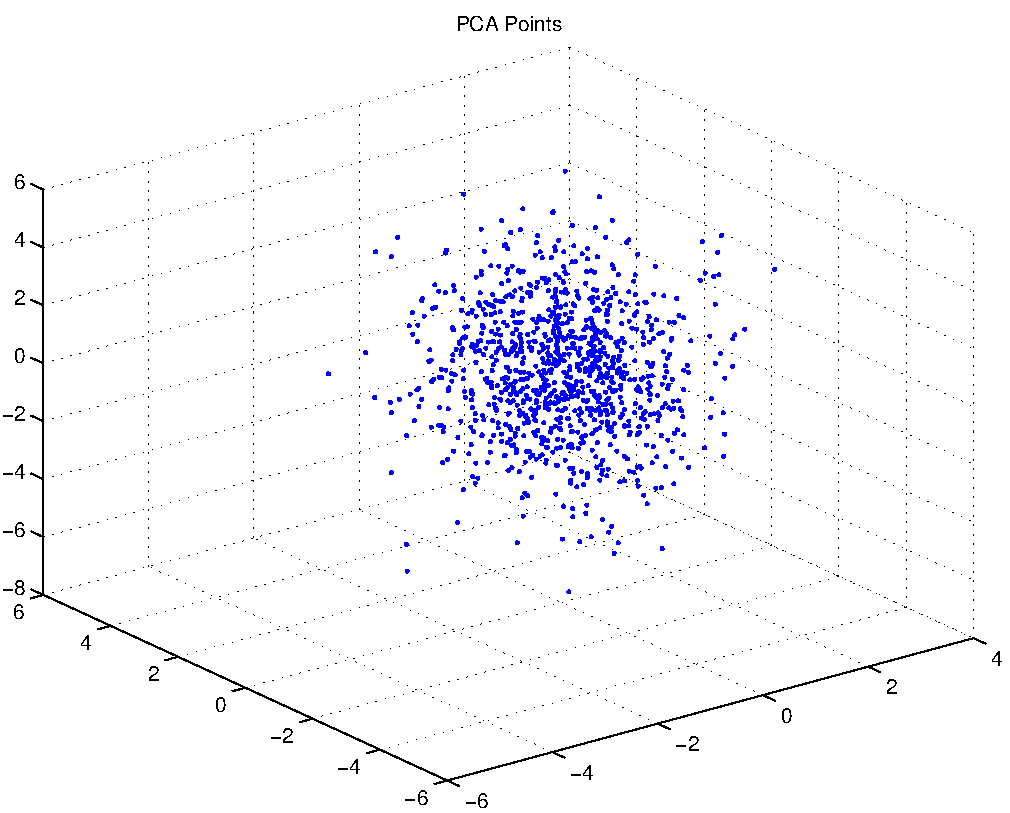
\includegraphics[width=10.0cm,height=10.0cm]{PCAPoints.pdf}

The eigenvectors:
+0.137, +0.282, +0.950
+0.098, +0.950, -0.296
-0.986, +0.134, +0.103

All of the eigenvalues of the covariance matrix:
(+0.958,+0.000), (+2.025,+0.000), (+3.017,+0.000)

QueryPerformanceCounter  =  +0.996
\subsubsection{Multi Variate Random Number Generator }
Sample from $N(\mu,\Sigma)$
mean= -0.002, variance=+1.004, skewness=+0.006, kurtosis=+3.003
mean= -0.001, variance=+1.017, skewness=-0.005, kurtosis=+2.988
mean= -0.002, variance=+1.006, skewness=-0.016, kurtosis=+3.014
Covariance Matrix 
+1.004, +0.009, +0.003
+0.009, +1.017, -0.003
+0.003, -0.003, +1.006

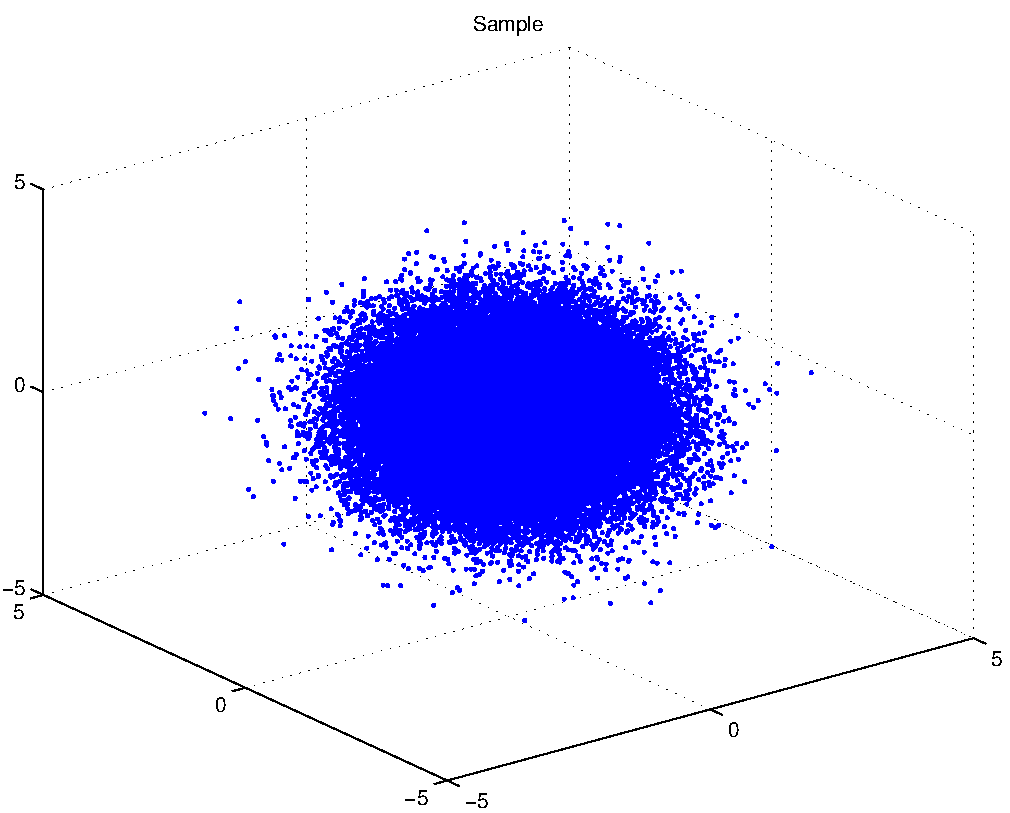
\includegraphics[width=10.0cm,height=10.0cm]{R_3_Normal.pdf}

Generate a sample from a unifom mixture of three Gaussians in $R^3$
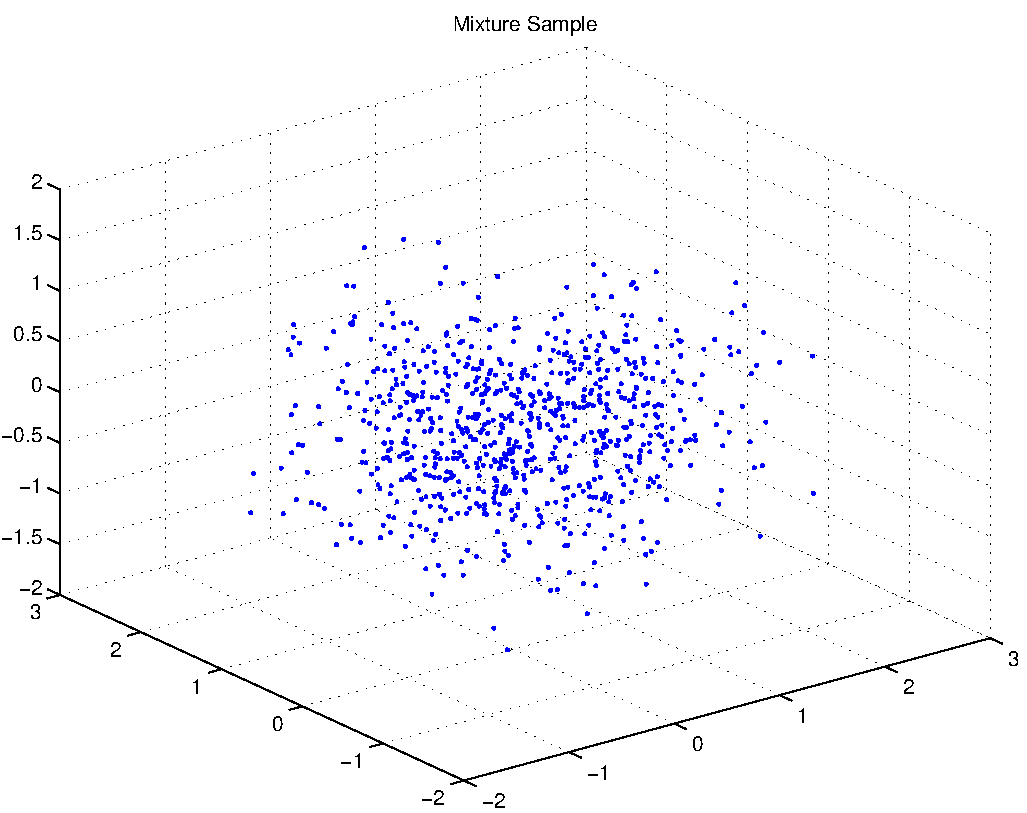
\includegraphics[width=10.0cm,height=10.0cm]{R_3_Normal_Mixture.pdf}

QueryPerformanceCounter  =  +14.931
\subsubsection{Matrix Multiply}
Comparing naive matrix multiply verus Intel MKL dgemm for matrix of size +2048.
This is for type double (hence the d in dgemm).
Naive type double matrix multiply tic toc  =  +0.513
dgemm plus row to column major transpose operation tic toc  =  +0.285
Comparing naive matrix multiply verus Intel MKL sgemm for matrix of size +2048.
This is for type float (hence the s in dgemm).
Naive type float matrix multiply tic toc  =  +0.257
sgemm plus row to column major transpose operation tic toc  =  +0.199
QueryPerformanceCounter  =  +1.391
\subsubsection{Descriptive Statistics}
Mean N(0,1): +0.003
Variance N(0,1): +1.006
Mean N(0,1) [recurrence relation method] :+0.003
Variance [recurrence relation method] :+1.006
Skewness : +0.007
Kurtosis : +2.997
QueryPerformanceCounter  =  +0.019
\subsubsection{Time Series }
+0.093
+0.726
+0.011
+2.178
QueryPerformanceCounter  =  +0.029
QueryPerformanceCounter  =  +6.229
\subsubsection{Iterated Exponential Filtering }
$\mu_1 =+0.093$
$\mu_2 =+0.726$
$\mu_3 =+0.011$
$\mu_4 =+2.178$
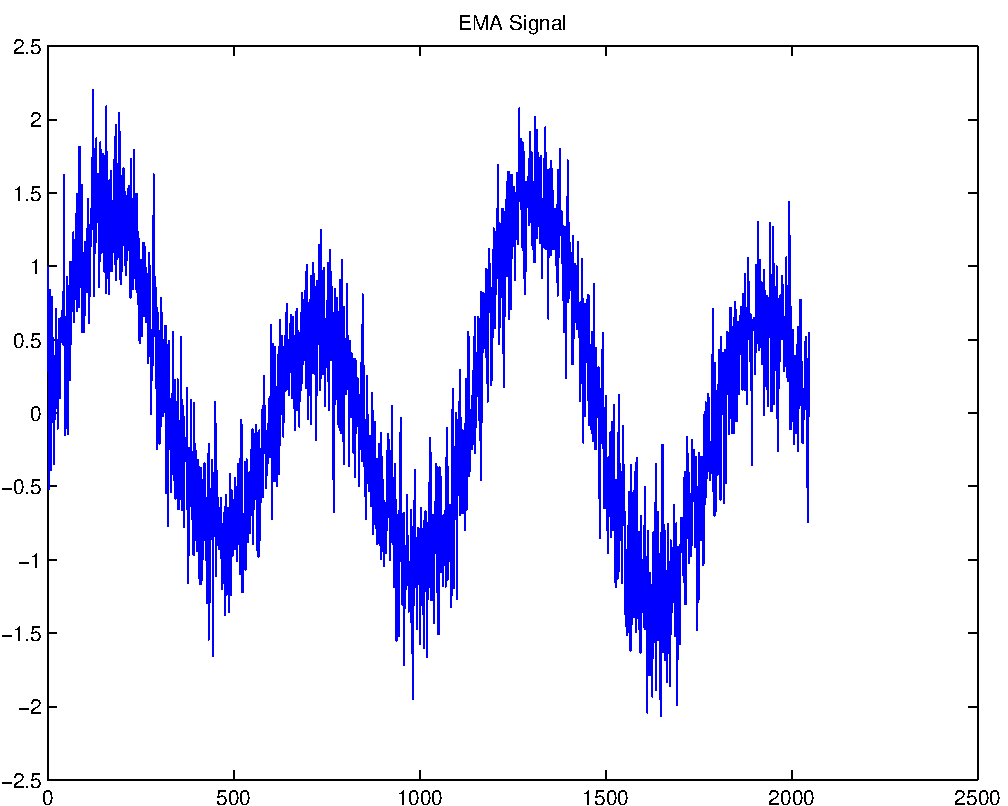
\includegraphics[width=10.0cm,height=10.0cm]{EMA_signal.pdf}

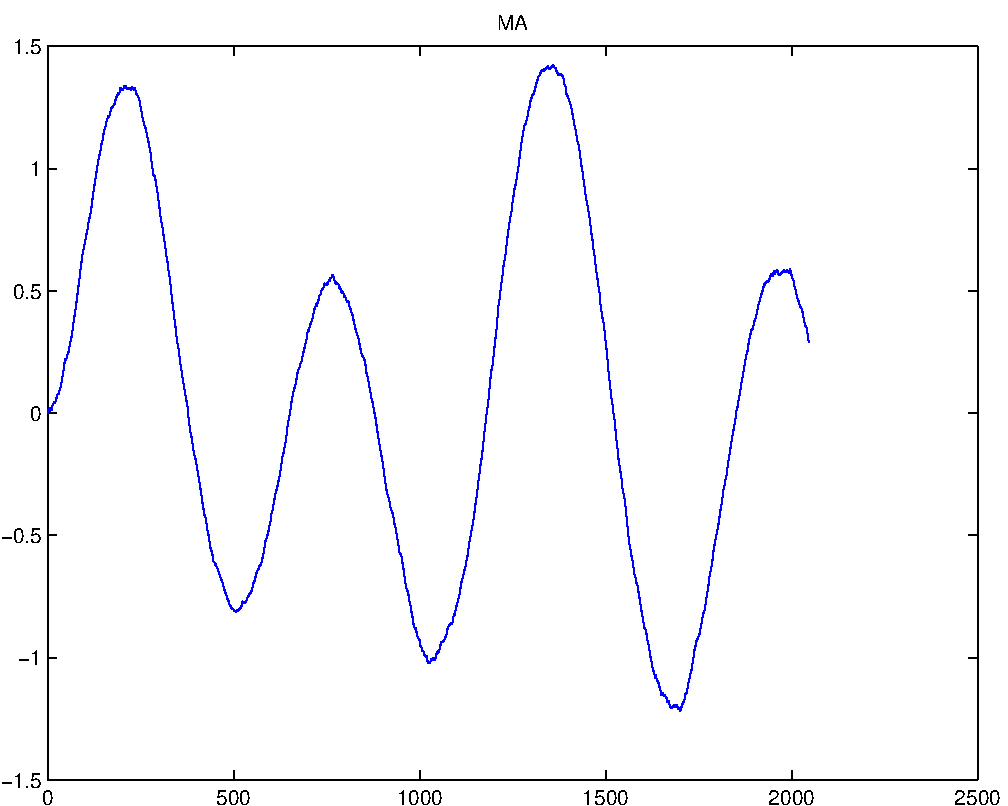
\includegraphics[width=10.0cm,height=10.0cm]{MA.pdf}

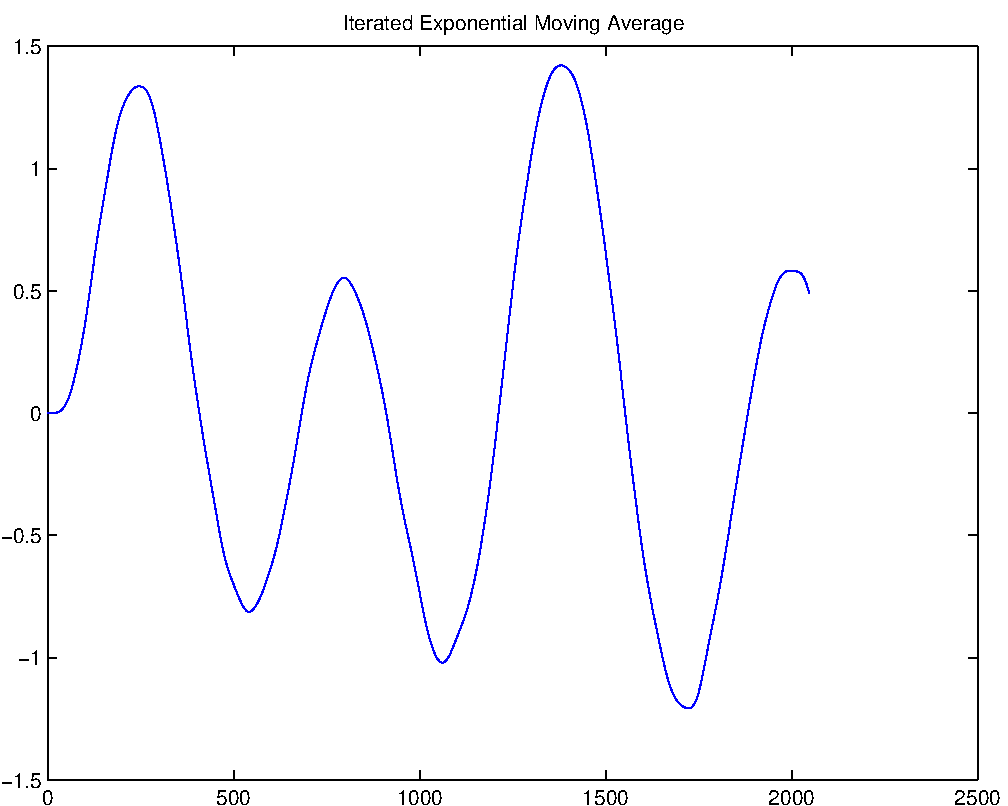
\includegraphics[width=10.0cm,height=10.0cm]{IEMA.pdf}

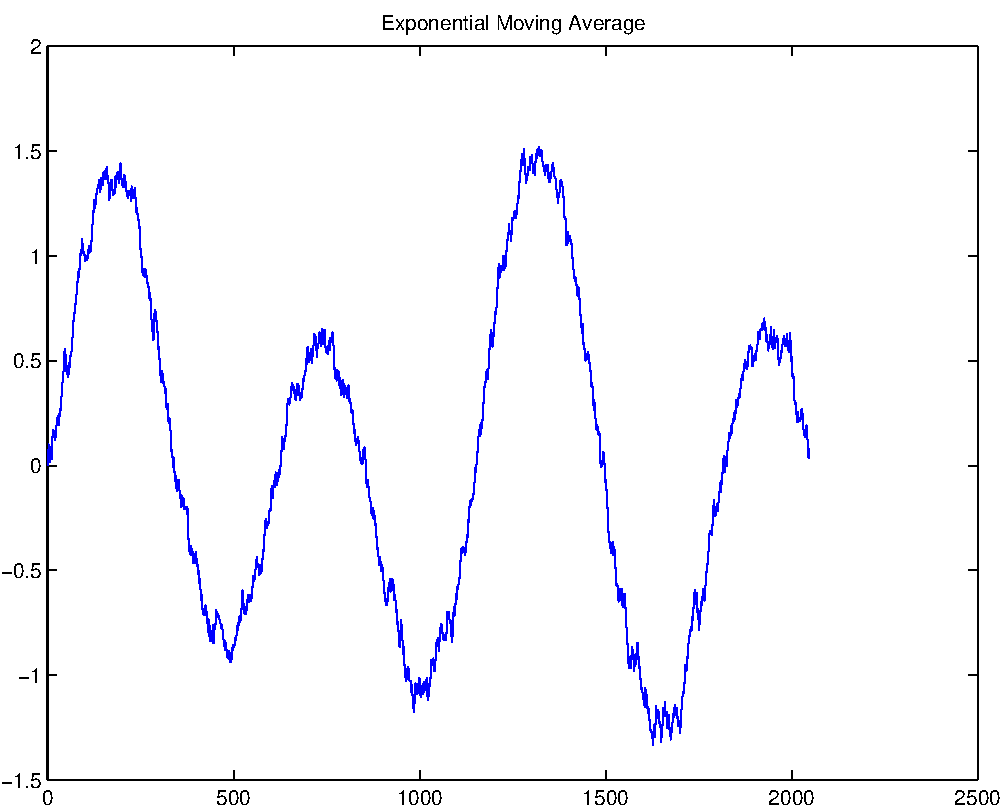
\includegraphics[width=10.0cm,height=10.0cm]{EMA.pdf}

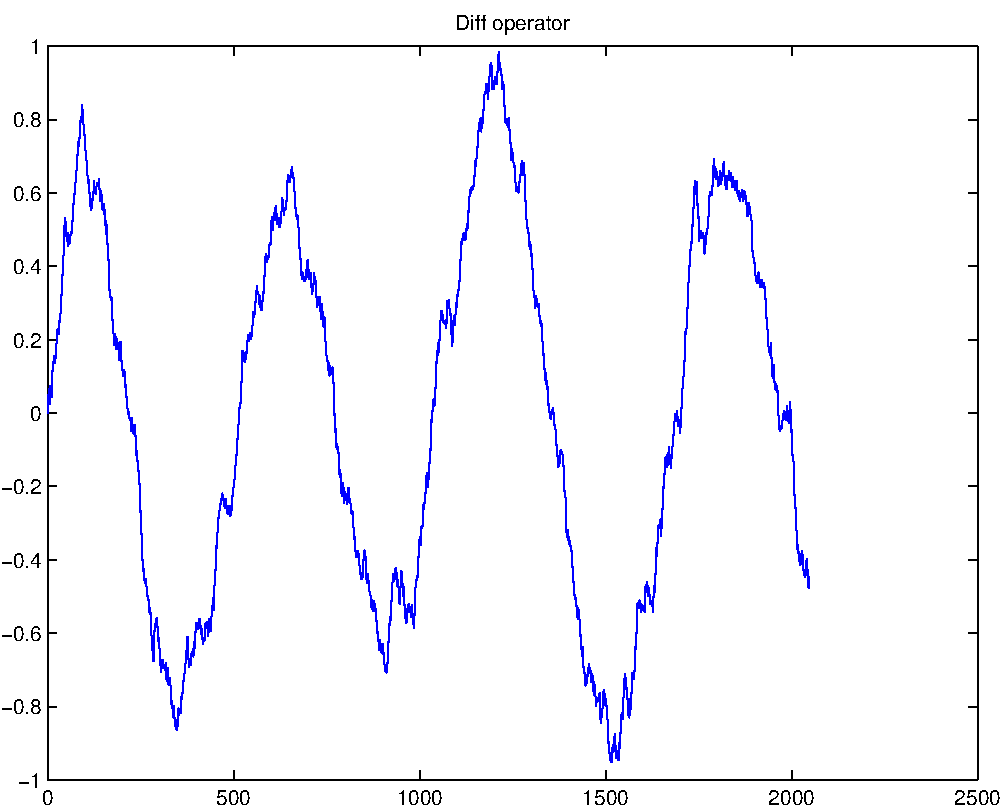
\includegraphics[width=10.0cm,height=10.0cm]{DIFF.pdf}

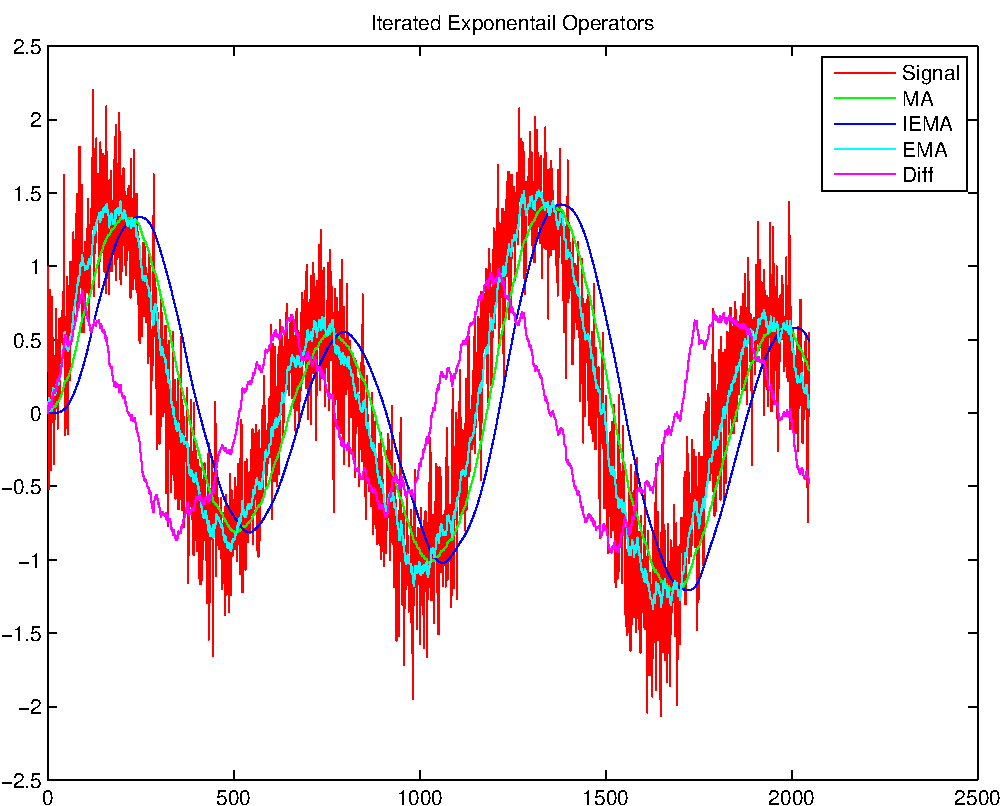
\includegraphics[width=10.0cm,height=10.0cm]{IteratedExponentailOperators.pdf}

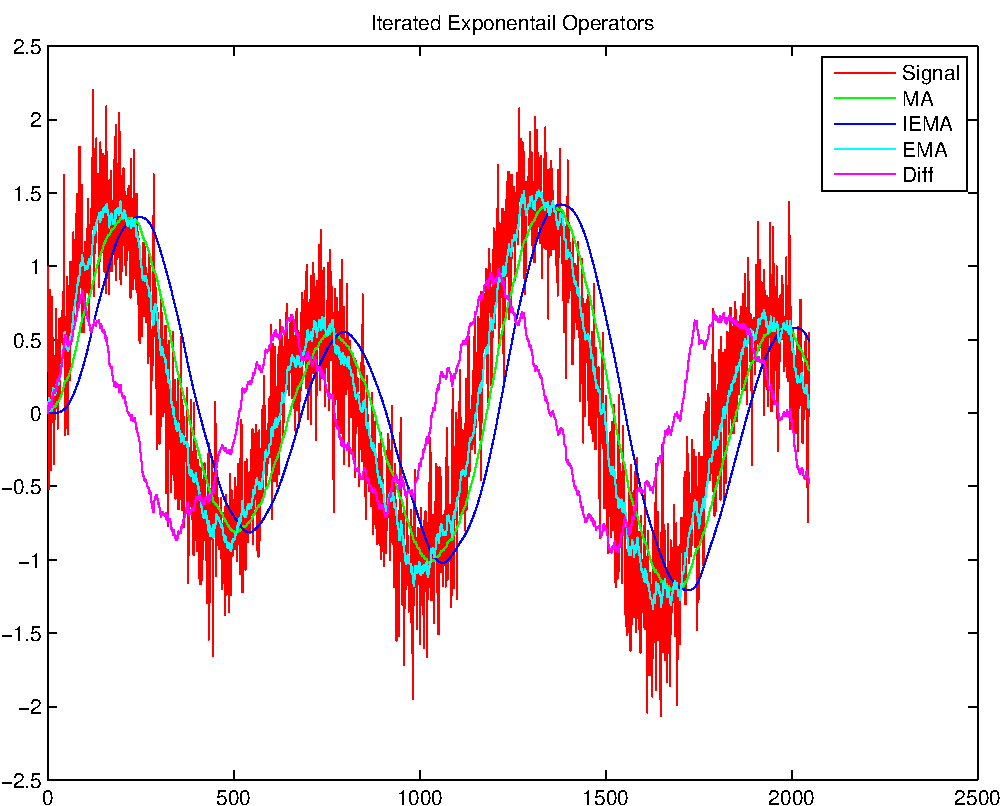
\includegraphics[width=10.0cm,height=10.0cm]{IteratedExponentailOperators.pdf}

QueryPerformanceCounter  =  +8.054
\subsubsection{Testing binary writer}
Binary writer Speedup 1GB Double Matrix +52.551

Binary reader Speedup 1GB Double Matrix +200.106

Binary writer Speedup 1GB Double vector +51.149

Binary reader Speedup 1GB Double Matrix +179.335

QueryPerformanceCounter  =  +0.909
\subsubsection{Testing Gaussian Mixture Point Cloud and Latex Plotting Capabilities.}
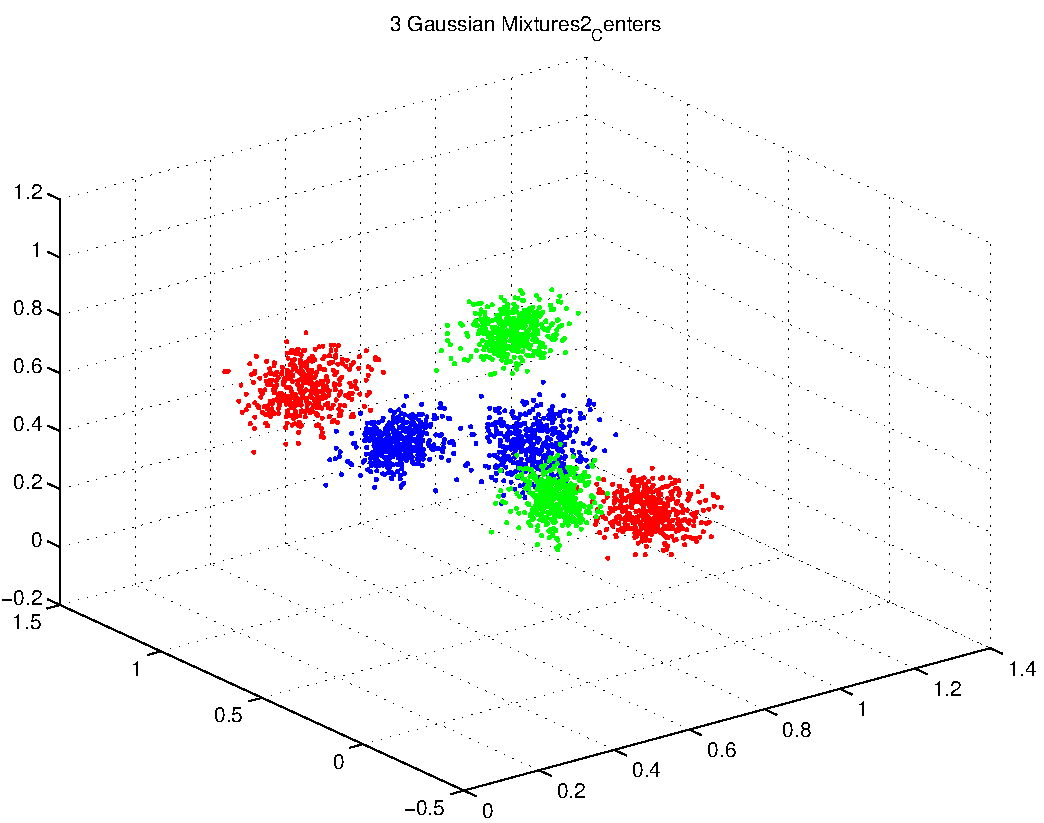
\includegraphics[width=10.0cm,height=10.0cm]{GaussianMixture_Dim_3_Centers2.pdf}

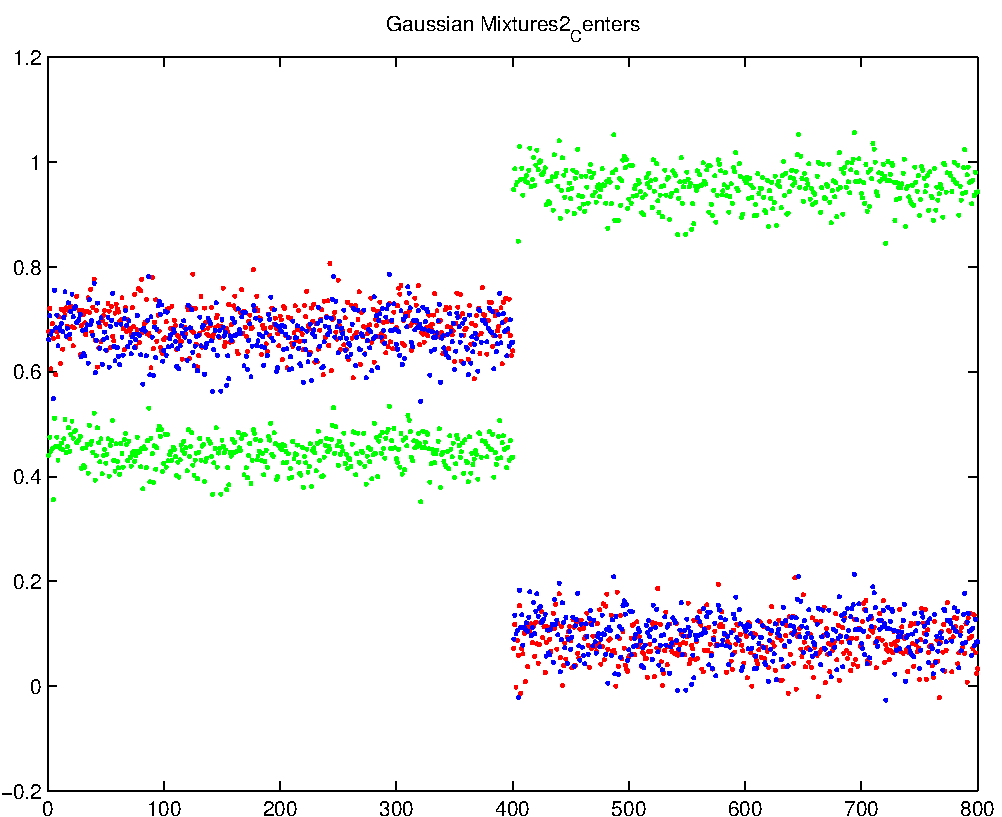
\includegraphics[width=10.0cm,height=10.0cm]{GaussianMixture_Dim_1_Centers2.pdf}

QueryPerformanceCounter  =  +2.697
\subsubsection{Intel VSL Function Check}
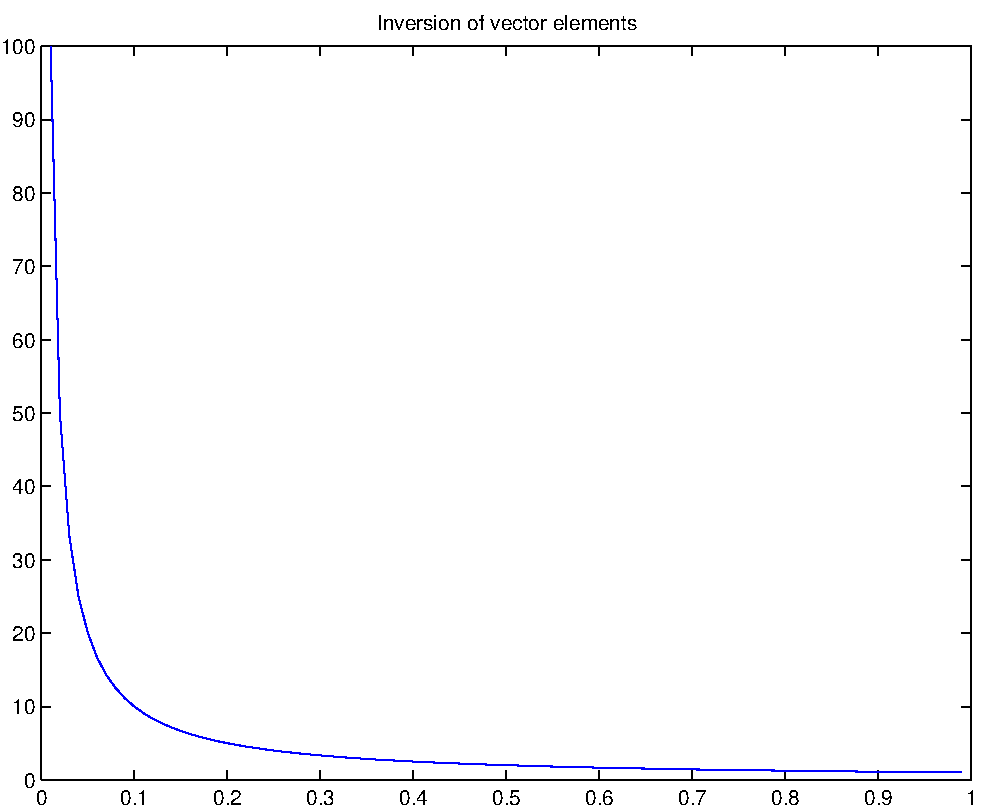
\includegraphics[width=10.0cm,height=10.0cm]{klVSLInv.pdf}

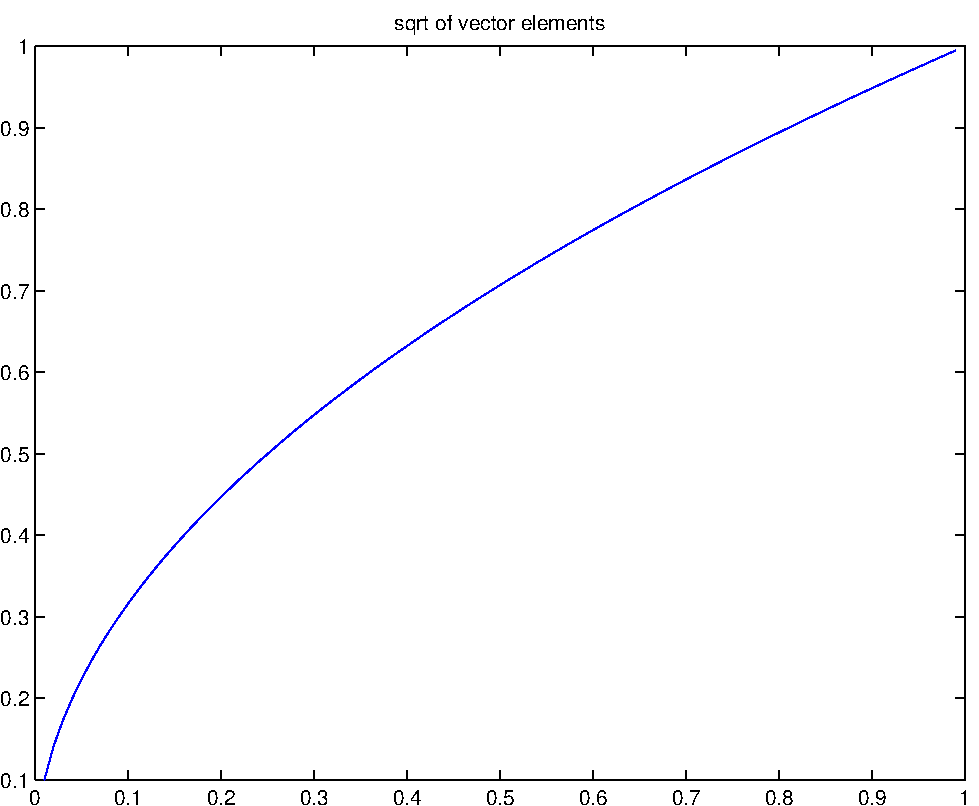
\includegraphics[width=10.0cm,height=10.0cm]{klVSLSqrt.pdf}

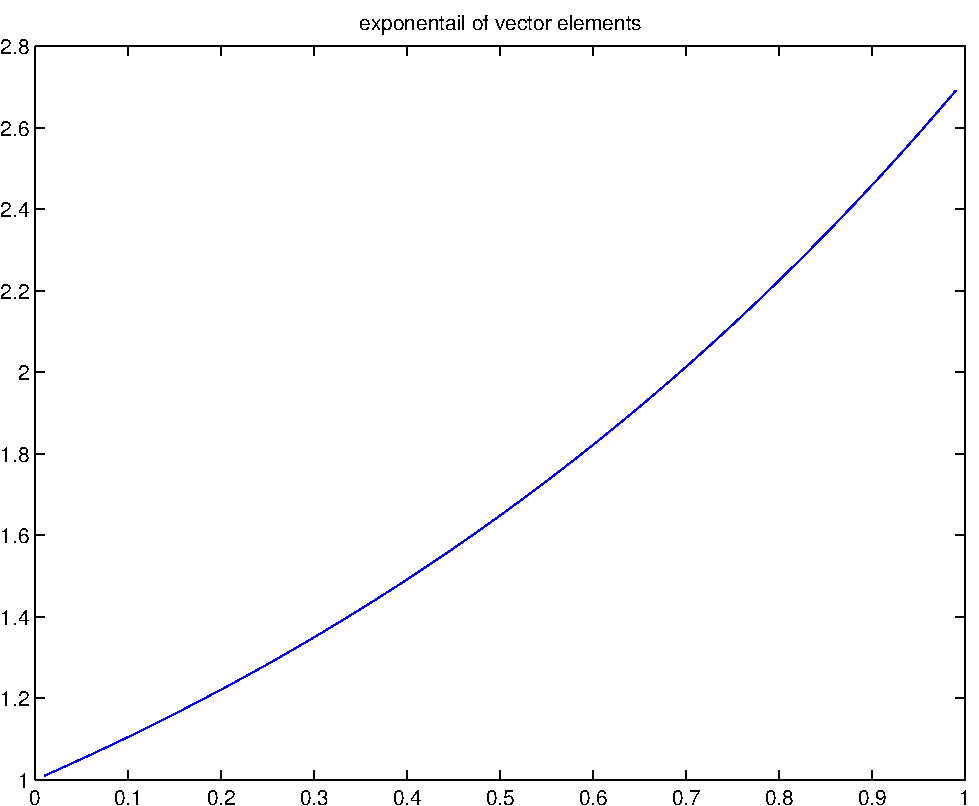
\includegraphics[width=10.0cm,height=10.0cm]{klVSLExp.pdf}

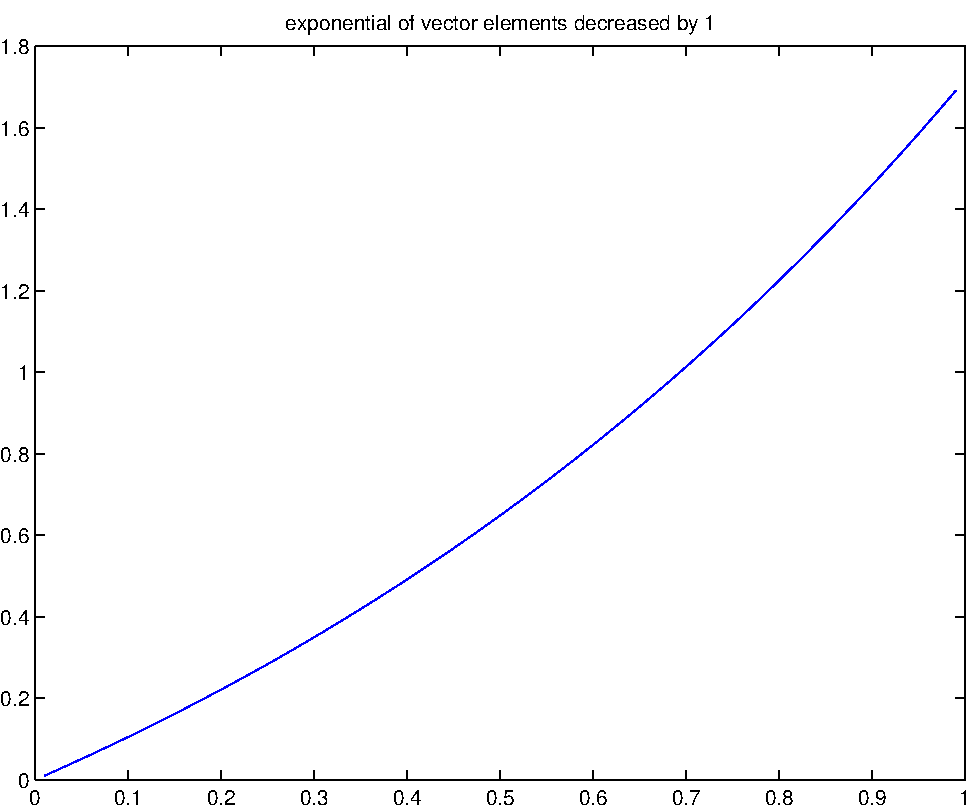
\includegraphics[width=10.0cm,height=10.0cm]{klVSLExpm1.pdf}

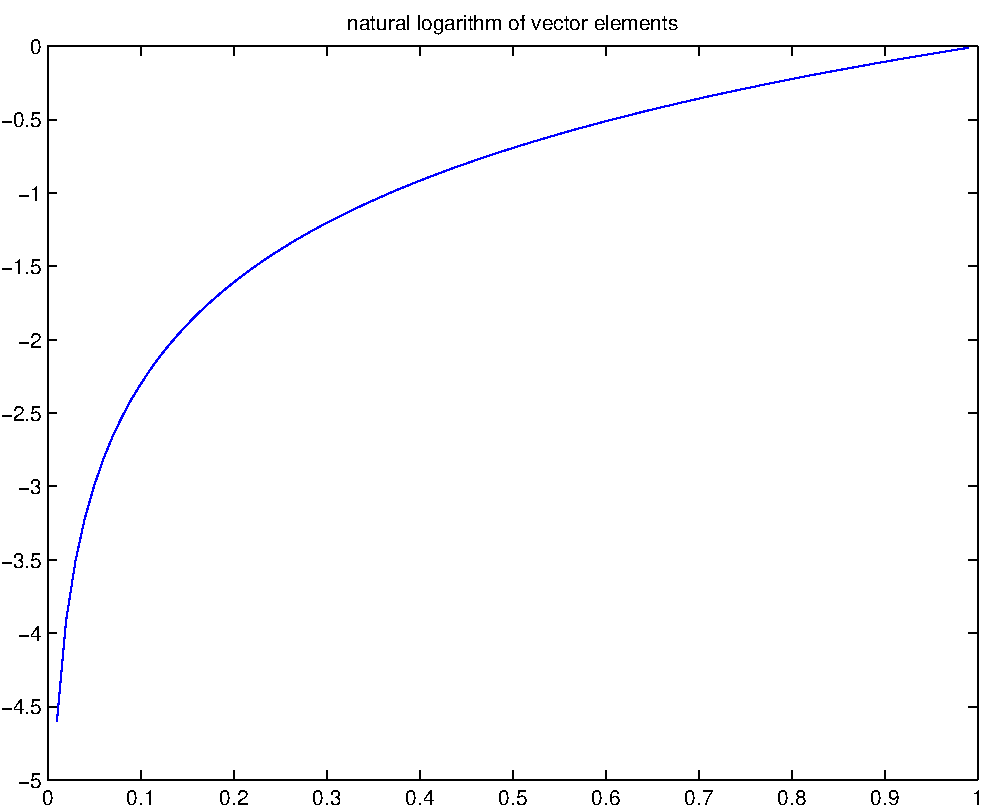
\includegraphics[width=10.0cm,height=10.0cm]{klVSLLn.pdf}

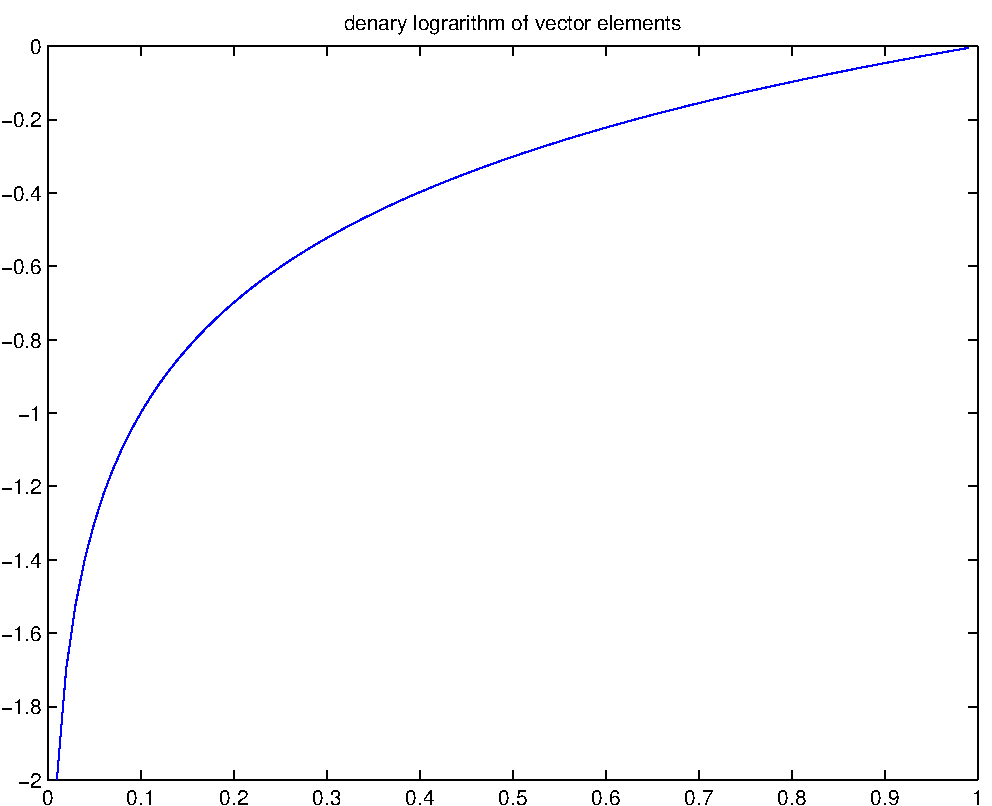
\includegraphics[width=10.0cm,height=10.0cm]{klVSLLog10.pdf}

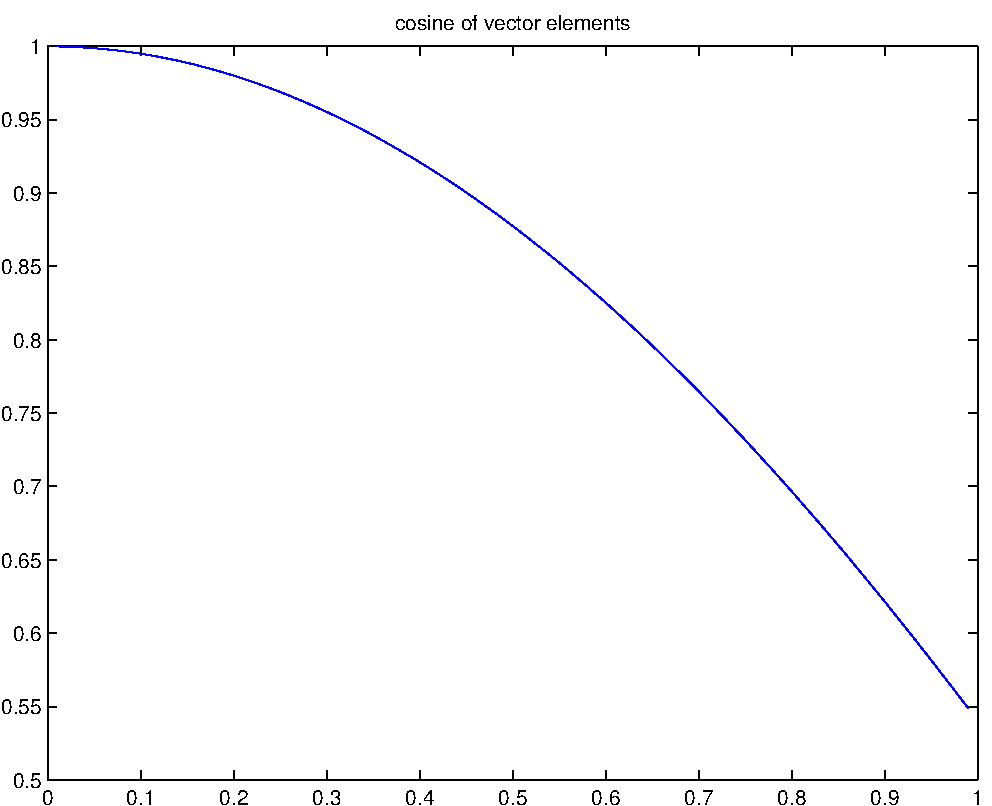
\includegraphics[width=10.0cm,height=10.0cm]{klVSLCos.pdf}

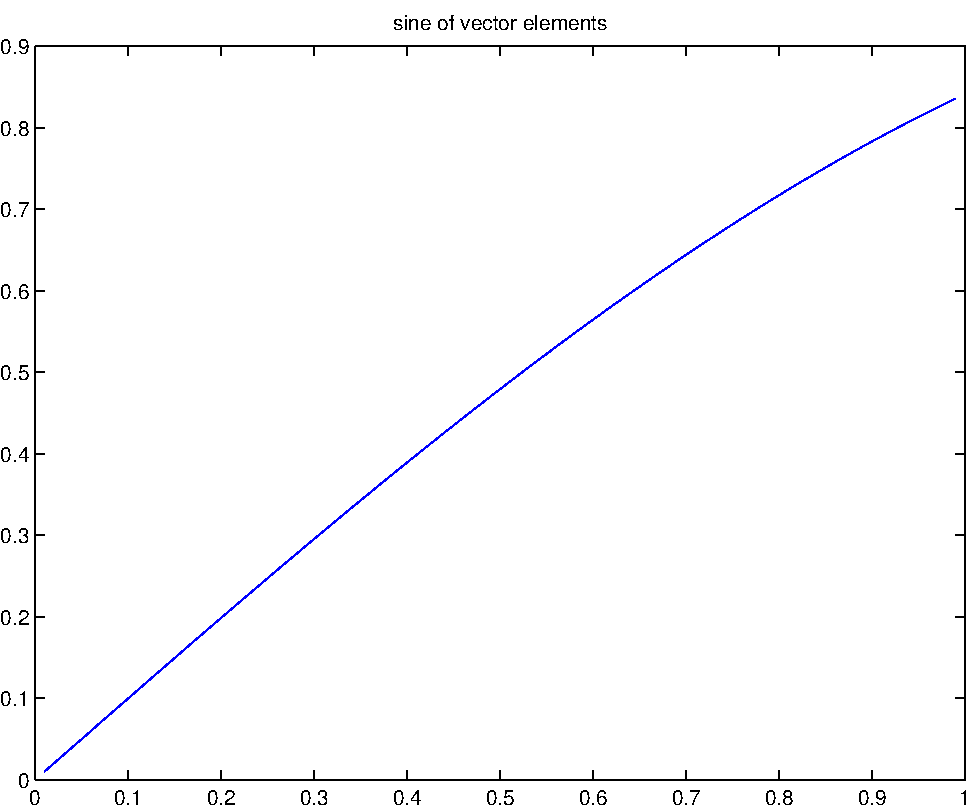
\includegraphics[width=10.0cm,height=10.0cm]{klVSLSin.pdf}

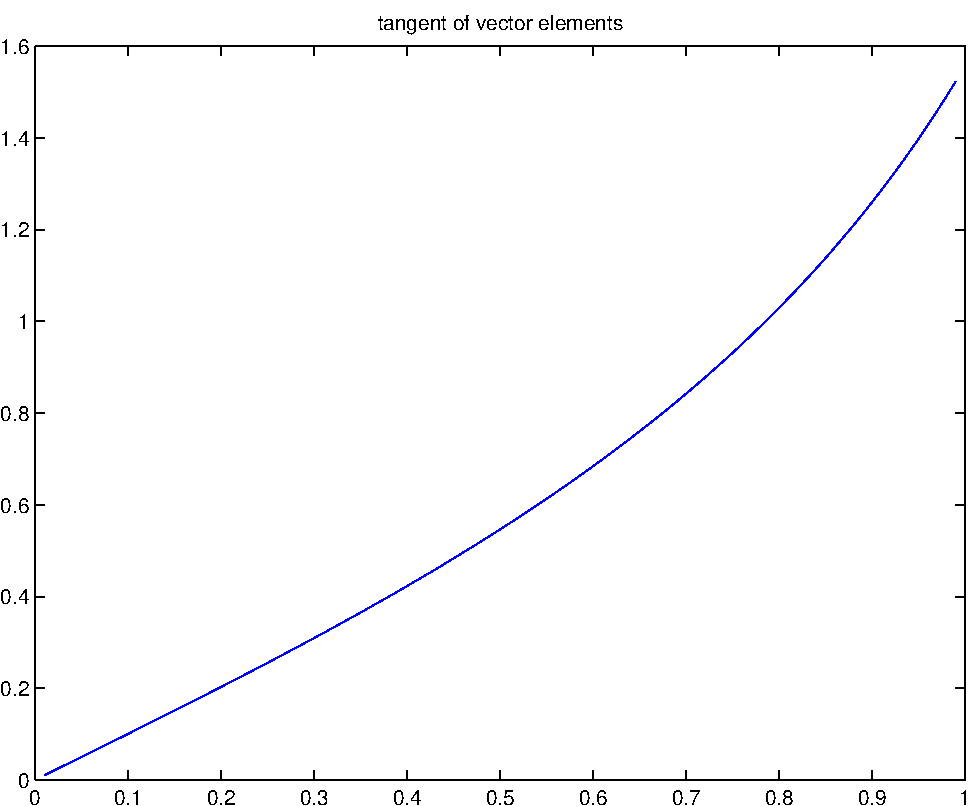
\includegraphics[width=10.0cm,height=10.0cm]{klVSLTan.pdf}

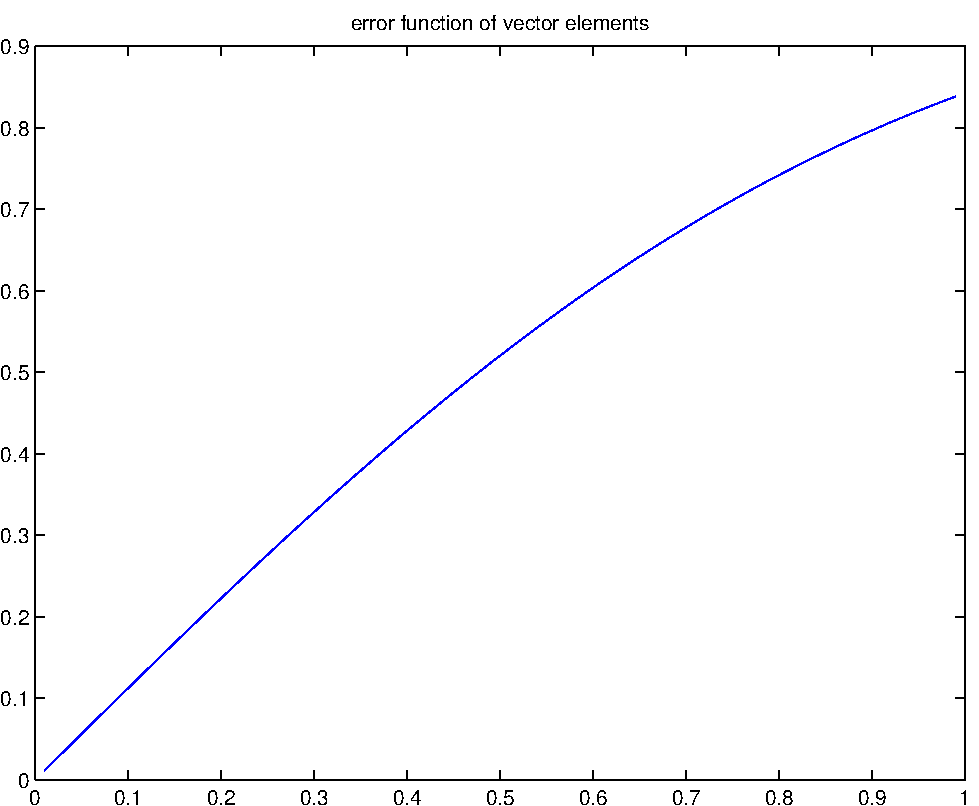
\includegraphics[width=10.0cm,height=10.0cm]{klVSLErf.pdf}

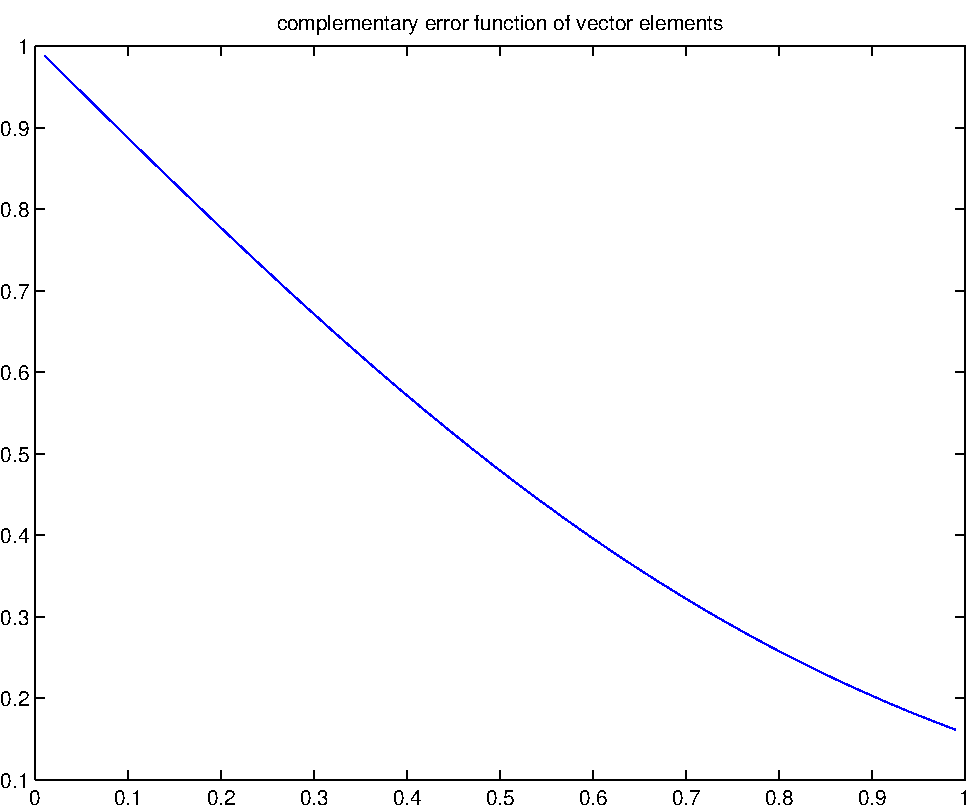
\includegraphics[width=10.0cm,height=10.0cm]{klVSLErfc.pdf}

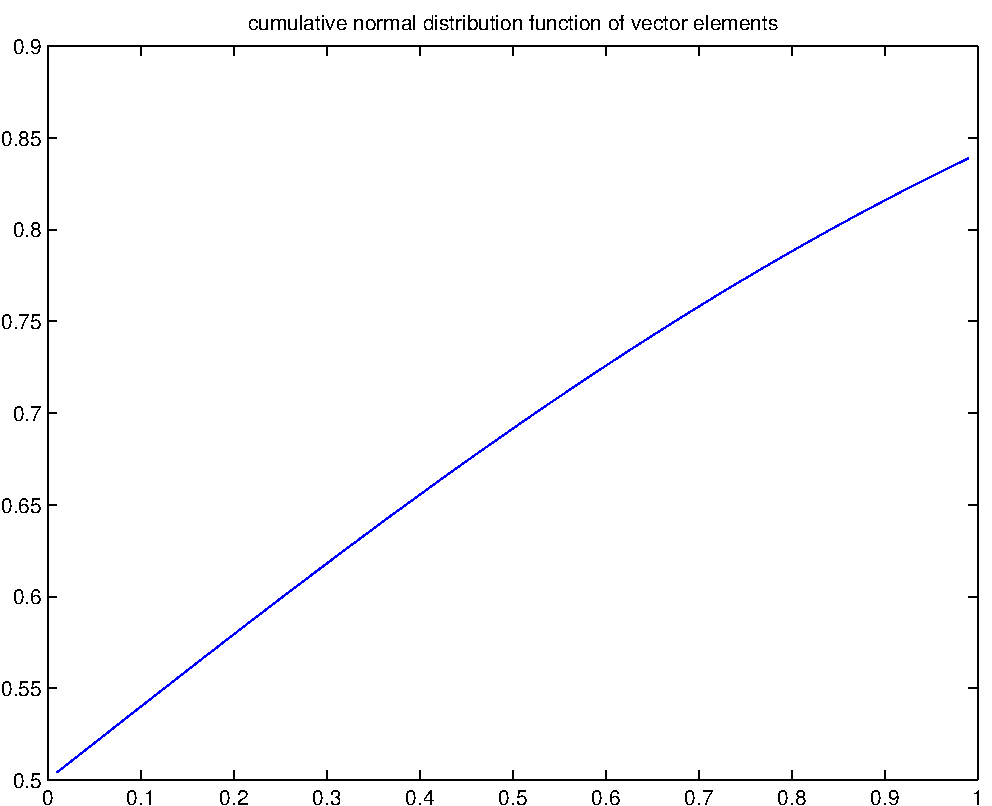
\includegraphics[width=10.0cm,height=10.0cm]{klVSLCdfNorm.pdf}

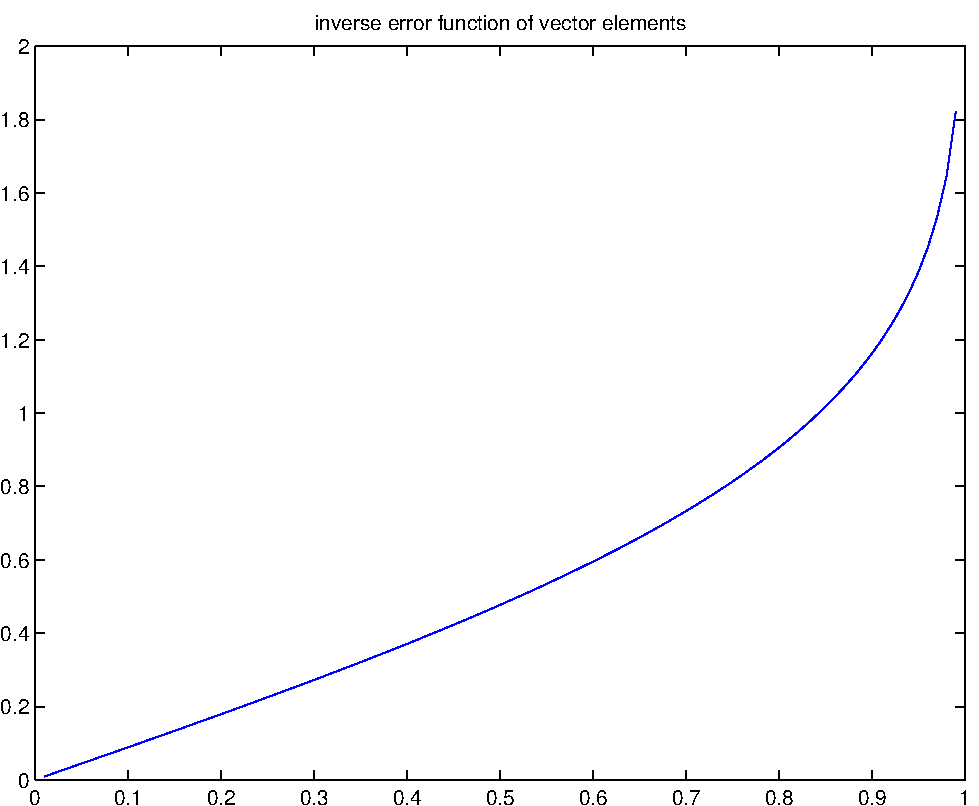
\includegraphics[width=10.0cm,height=10.0cm]{klVSLErfInv.pdf}

\includegraphics[width=10.0cm,height=10.0cm]{klVSLLGamma.pdf}

\includegraphics[width=10.0cm,height=10.0cm]{klVSLTGamma.pdf}

QueryPerformanceCounter  =  +14.716
\subsubsection{Gram Matrix Consistency Check}
Sample Size = 4096
Feature dim = 3

$$Sigma$ = \left(
\begin{array}{
ccc}
+1.140 & +1.535 & +0.581 \\
+1.535 & +9.988 & +1.605 \\
+0.581 & +1.605 & +0.428 \\
\end{array}
\right)$ \newline 

$Sample Covariance = \left(
\begin{array}{
ccc}
+1.143 & +1.550 & +0.588 \\
+1.550 & +10.091 & +1.624 \\
+0.588 & +1.624 & +0.435 \\
\end{array}
\right)$ \newline 

$Sample Mean = \left(
\begin{array}{
ccc}
+0.99112 & +0.95624 & +0.99057 \\
\end{array}
\right)$ \newline 

$Sample Covariance-$Omega$ = \left(
\begin{array}{
ccc}
+0.003 & +0.014 & +0.007 \\
+0.014 & +0.102 & +0.019 \\
+0.007 & +0.019 & +0.007 \\
\end{array}
\right)$ \newline 

$Sample Covariance Eigs = \left(
\begin{array}{
ccc}
(+10.63484,+0.00000) & (+0.99302,+0.00000) & (+0.04036,+0.00000) \\
\end{array}
\right)$ \newline 

$Centered Mean = \left(
\begin{array}{
ccc}
+0.00000 & -0.00000 & -0.00000 \\
\end{array}
\right)$ \newline 

$Centered Covariance = \left(
\begin{array}{
ccc}
+1.143 & +1.550 & +0.588 \\
+1.550 & +10.091 & +1.624 \\
+0.588 & +1.624 & +0.435 \\
\end{array}
\right)$ \newline 

$Gram Matrix Gf Not scaled by sample size = \left(
\begin{array}{
ccc}
+4680.484 & +6345.358 & +2407.603 \\
+6345.358 & +41331.679 & +6651.204 \\
+2407.603 & +6651.204 & +1780.905 \\
\end{array}
\right)$ \newline 

$Gram Matrix Gf  scaled by sample size = \left(
\begin{array}{
ccc}
+1.143 & +1.549 & +0.588 \\
+1.549 & +10.091 & +1.624 \\
+0.588 & +1.624 & +0.435 \\
\end{array}
\right)$ \newline 

$SampleCovariance - Scaled Gf = \left(
\begin{array}{
ccc}
+0.000 & +0.000 & +0.000 \\
+0.000 & +0.002 & +0.000 \\
+0.000 & +0.000 & +0.000 \\
\end{array}
\right)$ \newline 

$EigenDecomp of SampleCovariance = \left(
\begin{array}{
ccc}
-0.169 & -0.972 & -0.164 \\
+0.917 & -0.216 & +0.336 \\
-0.362 & -0.094 & +0.927 \\
\end{array}
\right)$ \newline 

$EigenDecomp of Gram Matrix = \left(
\begin{array}{
ccc}
-0.115 & -0.976 & -0.187 \\
-0.308 & +0.214 & -0.927 \\
+0.944 & -0.049 & -0.325 \\
\end{array}
\right)$ \newline 

QueryPerformanceCounter  =  +1.324
\subsubsection{Eigen Solver Checks}
\subsubsection{Haar Distributed Random Orthogonal Matrix $A \in O(n)$}
 Testing Operator Norm
Number of Dimensions: +8

$A = \left(
\begin{array}{
cccccccc}
-0.562 & +0.252 & +0.164 & -0.574 & -0.232 & +0.197 & -0.141 & -0.389 \\
-0.466 & +0.165 & -0.616 & +0.244 & +0.296 & +0.285 & +0.383 & -0.011 \\
-0.146 & -0.098 & -0.023 & +0.482 & -0.142 & +0.459 & -0.711 & +0.002 \\
+0.143 & -0.556 & -0.446 & -0.496 & +0.348 & +0.062 & -0.304 & -0.090 \\
-0.178 & -0.660 & +0.141 & +0.277 & -0.243 & -0.048 & +0.328 & -0.518 \\
+0.332 & +0.383 & -0.328 & +0.167 & -0.003 & -0.298 & -0.191 & -0.694 \\
-0.224 & +0.020 & +0.469 & +0.146 & +0.796 & -0.150 & -0.130 & -0.185 \\
-0.483 & -0.092 & -0.217 & +0.084 & -0.151 & -0.743 & -0.273 & +0.236 \\
\end{array}
\right)$ \newline 

$Det(A) :   A \in O(n)$ = (-1.000,+0.000)

$L = \left(
\begin{array}{
cccccccc}
+1.000 & +0.000 & +0.000 & +0.000 & +0.000 & +0.000 & +0.000 & +0.000 \\
+0.317 & +1.000 & +0.000 & +0.000 & +0.000 & +0.000 & +0.000 & +0.000 \\
+0.830 & +0.060 & +1.000 & +0.000 & +0.000 & +0.000 & +0.000 & +0.000 \\
-0.255 & +0.664 & +0.612 & +1.000 & +0.000 & +0.000 & +0.000 & +0.000 \\
+0.399 & +0.109 & -0.520 & -0.500 & +1.000 & +0.000 & +0.000 & +0.000 \\
+0.859 & +0.418 & +0.522 & -0.017 & -0.114 & +1.000 & +0.000 & +0.000 \\
+0.261 & +0.222 & +0.113 & -0.330 & -0.056 & -0.475 & +1.000 & +0.000 \\
-0.591 & -0.719 & +0.221 & -0.003 & -0.306 & +0.339 & +0.003 & +1.000 \\
\end{array}
\right)$ \newline 

$U = \left(
\begin{array}{
cccccccc}
-0.562 & +0.252 & +0.164 & -0.574 & -0.232 & +0.197 & -0.141 & -0.389 \\
+0.000 & -0.739 & +0.089 & +0.459 & -0.170 & -0.110 & +0.372 & -0.394 \\
+0.000 & +0.000 & -0.757 & +0.693 & +0.499 & +0.128 & +0.478 & +0.336 \\
+0.000 & +0.000 & +0.000 & -1.371 & +0.097 & +0.107 & -0.881 & -0.133 \\
+0.000 & +0.000 & +0.000 & +0.000 & +1.216 & -0.097 & -0.306 & +0.121 \\
+0.000 & +0.000 & +0.000 & +0.000 & +0.000 & -0.942 & -0.607 & +0.572 \\
+0.000 & +0.000 & +0.000 & +0.000 & +0.000 & +0.000 & -1.406 & +0.388 \\
+0.000 & +0.000 & +0.000 & +0.000 & +0.000 & +0.000 & +0.000 & -1.440 \\
\end{array}
\right)$ \newline 

$L * U  = \left(
\begin{array}{
cccccccc}
-0.562 & +0.252 & +0.164 & -0.574 & -0.232 & +0.197 & -0.141 & -0.389 \\
-0.178 & -0.660 & +0.141 & +0.277 & -0.243 & -0.048 & +0.328 & -0.518 \\
-0.466 & +0.165 & -0.616 & +0.244 & +0.296 & +0.285 & +0.383 & -0.011 \\
+0.143 & -0.556 & -0.446 & -0.496 & +0.348 & +0.062 & -0.304 & -0.090 \\
-0.224 & +0.020 & +0.469 & +0.146 & +0.796 & -0.150 & -0.130 & -0.185 \\
-0.483 & -0.092 & -0.217 & +0.084 & -0.151 & -0.743 & -0.273 & +0.236 \\
-0.146 & -0.098 & -0.023 & +0.482 & -0.142 & +0.459 & -0.711 & +0.002 \\
+0.332 & +0.383 & -0.328 & +0.167 & -0.003 & -0.298 & -0.191 & -0.694 \\
\end{array}
\right)$ \newline 

$Det(L) :    = (+1.000,+0.000)     Det(U) :    = (-1.000,+0.000)     Det(LU) :    = (-1.000,+0.000)$

$||A||_{L_1}$  = +2.534

$||A||_{L_{\infty}}$ = +2.512

$||A^{-1}||_{L_1}$  = +2.512

$||A^{-1}||_{L_{\infty}}$ = +2.534

$||A||_{L_{\infty}} * ||A^{-1}||_{L_{\infty}} = +6.366$

$||A||_{L_1} * ||A^{-1}||_{L_1} = +6.366$

Frobenious Norm  $||A||_{\textit{F}}$ via $\sum\limits_{i,j =0}^{n} \|A_{i,j}|$   of  $A \in O(n)$  +2.828

$L_1$ condition number of Haar Distributed Random Orthogonal Matrix $A \in O(n)$ +5.773

$A = \left(
\begin{array}{
cccccccc}
-0.562 & +0.252 & +0.164 & -0.574 & -0.232 & +0.197 & -0.141 & -0.389 \\
-0.466 & +0.165 & -0.616 & +0.244 & +0.296 & +0.285 & +0.383 & -0.011 \\
-0.146 & -0.098 & -0.023 & +0.482 & -0.142 & +0.459 & -0.711 & +0.002 \\
+0.143 & -0.556 & -0.446 & -0.496 & +0.348 & +0.062 & -0.304 & -0.090 \\
-0.178 & -0.660 & +0.141 & +0.277 & -0.243 & -0.048 & +0.328 & -0.518 \\
+0.332 & +0.383 & -0.328 & +0.167 & -0.003 & -0.298 & -0.191 & -0.694 \\
-0.224 & +0.020 & +0.469 & +0.146 & +0.796 & -0.150 & -0.130 & -0.185 \\
-0.483 & -0.092 & -0.217 & +0.084 & -0.151 & -0.743 & -0.273 & +0.236 \\
\end{array}
\right)$ \newline 

$L_{\infty}$ condition number of Haar Distributed Random Orthogonal Matrix $A \in O(n)$ +6.183

Eigenvalues of $A \in O(n)$

(+0.553,+0.833), (+0.553,-0.833), (-0.260,+0.966), (-0.260,-0.966), (-0.969,+0.248), (-0.969,-0.248), (-1.000,+0.000), (+1.000,+0.000)

 $|\lambda | : \lambda \in \sigma(A) , A \in O(n)$

+1.000, +1.000, +1.000, +1.000, +1.000, +1.000, +1.000, +1.000


Calculating $A^{\dag} A,$  we expect $A^{\dag} A \approx I$

$A^{\dag} A = \left(
\begin{array}{
cccccccc}
+1.000 & -0.000 & +0.000 & +0.000 & +0.000 & +0.000 & +0.000 & -0.000 \\
-0.000 & +1.000 & +0.000 & +0.000 & -0.000 & +0.000 & -0.000 & -0.000 \\
+0.000 & +0.000 & +1.000 & +0.000 & -0.000 & -0.000 & -0.000 & +0.000 \\
+0.000 & +0.000 & +0.000 & +1.000 & -0.000 & +0.000 & +0.000 & +0.000 \\
+0.000 & -0.000 & -0.000 & -0.000 & +1.000 & -0.000 & -0.000 & +0.000 \\
+0.000 & +0.000 & -0.000 & +0.000 & -0.000 & +1.000 & -0.000 & -0.000 \\
+0.000 & -0.000 & -0.000 & +0.000 & -0.000 & -0.000 & +1.000 & -0.000 \\
-0.000 & -0.000 & +0.000 & +0.000 & +0.000 & -0.000 & -0.000 & +1.000 \\
\end{array}
\right)$ \newline 

Calculating $A^{-1} ,  A \in O(n)$.

$A^{-1} = \left(
\begin{array}{
cccccccc}
-0.562 & -0.466 & -0.146 & +0.143 & -0.178 & +0.332 & -0.224 & -0.483 \\
+0.252 & +0.165 & -0.098 & -0.556 & -0.660 & +0.383 & +0.020 & -0.092 \\
+0.164 & -0.616 & -0.023 & -0.446 & +0.141 & -0.328 & +0.469 & -0.217 \\
-0.574 & +0.244 & +0.482 & -0.496 & +0.277 & +0.167 & +0.146 & +0.084 \\
-0.232 & +0.296 & -0.142 & +0.348 & -0.243 & -0.003 & +0.796 & -0.151 \\
+0.197 & +0.285 & +0.459 & +0.062 & -0.048 & -0.298 & -0.150 & -0.743 \\
-0.141 & +0.383 & -0.711 & -0.304 & +0.328 & -0.191 & -0.130 & -0.273 \\
-0.389 & -0.011 & +0.002 & -0.090 & -0.518 & -0.694 & -0.185 & +0.236 \\
\end{array}
\right)$ \newline 

Calculating $A^{-1} *A  ,  A \in O(n)$.   We expect $A^{-1} *A  \approx I$. 

$A^{-1} *A = \left(
\begin{array}{
cccccccc}
+1.000 & -0.000 & +0.000 & +0.000 & -0.000 & -0.000 & +0.000 & +0.000 \\
+0.000 & +1.000 & +0.000 & +0.000 & +0.000 & +0.000 & +0.000 & -0.000 \\
-0.000 & +0.000 & +1.000 & -0.000 & -0.000 & +0.000 & +0.000 & +0.000 \\
-0.000 & -0.000 & +0.000 & +1.000 & +0.000 & -0.000 & -0.000 & -0.000 \\
-0.000 & +0.000 & +0.000 & -0.000 & +1.000 & +0.000 & +0.000 & -0.000 \\
+0.000 & +0.000 & +0.000 & -0.000 & -0.000 & +1.000 & -0.000 & +0.000 \\
-0.000 & +0.000 & +0.000 & +0.000 & -0.000 & +0.000 & +1.000 & +0.000 \\
+0.000 & +0.000 & +0.000 & +0.000 & -0.000 & -0.000 & -0.000 & +1.000 \\
\end{array}
\right)$ \newline 

Calculating SVD of  $A \in O(n)$

$U = \left(
\begin{array}{
cccccccc}
-0.085 & -0.770 & -0.300 & -0.320 & -0.330 & +0.169 & -0.030 & +0.262 \\
-0.562 & +0.252 & +0.164 & -0.574 & -0.232 & +0.197 & -0.141 & -0.389 \\
-0.610 & -0.220 & -0.240 & +0.585 & -0.027 & -0.265 & -0.163 & -0.285 \\
-0.064 & +0.155 & -0.255 & +0.173 & +0.285 & +0.700 & -0.514 & +0.202 \\
+0.019 & +0.102 & +0.320 & +0.017 & -0.355 & -0.375 & -0.670 & +0.413 \\
+0.214 & +0.314 & -0.287 & +0.280 & -0.781 & +0.230 & +0.143 & -0.108 \\
-0.088 & +0.363 & -0.729 & -0.312 & +0.127 & -0.398 & -0.000 & +0.238 \\
+0.496 & -0.173 & -0.211 & -0.139 & +0.058 & -0.139 & -0.467 & -0.647 \\
\end{array}
\right)$ \newline 

$S = \left(
\begin{array}{
cccccccc}
+1.000 & +0.000 & +0.000 & +0.000 & +0.000 & +0.000 & +0.000 & +0.000 \\
+0.000 & +1.000 & +0.000 & +0.000 & +0.000 & +0.000 & +0.000 & +0.000 \\
+0.000 & +0.000 & +1.000 & +0.000 & +0.000 & +0.000 & +0.000 & +0.000 \\
+0.000 & +0.000 & +0.000 & +1.000 & +0.000 & +0.000 & +0.000 & +0.000 \\
+0.000 & +0.000 & +0.000 & +0.000 & +1.000 & +0.000 & +0.000 & +0.000 \\
+0.000 & +0.000 & +0.000 & +0.000 & +0.000 & +1.000 & +0.000 & +0.000 \\
+0.000 & +0.000 & +0.000 & +0.000 & +0.000 & +0.000 & +1.000 & +0.000 \\
+0.000 & +0.000 & +0.000 & +0.000 & +0.000 & +0.000 & +0.000 & +1.000 \\
\end{array}
\right)$ \newline 

$V = \left(
\begin{array}{
cccccccc}
-0.000 & +1.000 & -0.000 & +0.000 & +0.000 & +0.000 & -0.000 & -0.000 \\
-0.045 & +0.000 & +0.396 & +0.340 & -0.659 & +0.087 & +0.395 & -0.358 \\
+0.087 & +0.000 & +0.396 & +0.730 & +0.344 & +0.194 & -0.357 & +0.141 \\
+0.589 & +0.000 & -0.099 & +0.214 & -0.185 & -0.446 & +0.264 & +0.543 \\
+0.319 & +0.000 & +0.495 & -0.455 & -0.350 & +0.074 & -0.549 & +0.131 \\
-0.504 & +0.000 & +0.198 & -0.101 & -0.102 & +0.314 & +0.250 & +0.725 \\
-0.516 & +0.000 & +0.198 & +0.074 & -0.066 & -0.790 & -0.243 & +0.014 \\
+0.145 & +0.000 & +0.594 & -0.289 & +0.526 & -0.164 & +0.474 & -0.120 \\
\end{array}
\right)$ \newline 

$U S V = \left(
\begin{array}{
cccccccc}
-0.317 & -0.085 & -0.372 & -0.494 & +0.701 & +0.027 & +0.073 & +0.108 \\
-0.492 & -0.562 & -0.114 & +0.271 & -0.138 & +0.530 & -0.084 & -0.222 \\
+0.502 & -0.610 & -0.507 & -0.015 & -0.149 & -0.236 & +0.006 & +0.199 \\
+0.105 & -0.064 & +0.241 & -0.393 & -0.253 & +0.501 & +0.438 & +0.516 \\
+0.515 & +0.019 & +0.028 & +0.302 & +0.463 & +0.382 & +0.391 & -0.360 \\
-0.328 & +0.214 & -0.394 & +0.332 & -0.174 & -0.234 & +0.700 & +0.078 \\
+0.012 & -0.088 & +0.012 & -0.562 & -0.310 & -0.125 & +0.265 & -0.703 \\
+0.144 & +0.496 & -0.614 & -0.102 & -0.249 & +0.442 & -0.289 & -0.065 \\
\end{array}
\right)$ \newline 

Calculating first few eigenvectors of $A \in O(n)$ using LAPACK syevx

\subsubsection{Wishart Matrix $A \in W(n)$}
$L_1$ condition number of Wishart Matrix +1489.694
$L_infty$ condition number of Wishart Matrix +1489.694
\subsubsection{Gaussian Orthogonal Ensemble $A \in GOE(n)$}
$L_1$ condition number of GOE Matrix +66.900
$L_\infty$ condition number of GOE Matrix +66.900
\subsubsection{The Identity Matrix $I \in M(n)$}
$L_1$ condition number of $I$ = +1.000
$L_\infty$ condition number of $I$ = +1.000
QueryPerformanceCounter  =  +0.310
\subsubsection{Generate Tracey Widom Sample}
\subsubsection{Sample from $W_n m$ times and calculate empirical PDF of the first eig}
Here we generate histograms of $\lambda_1$ for GOE (Gaussian Orthogonal Ensemble), and W (Wishart) 		 distributed of random matrices
These should approximate the celebrated Tracy Widom distribution.
Dimension $n = +128$

Sample size $m = 32$

\includegraphics[width=10.0cm,height=10.0cm]{Re_TraceyWidom.pdf}

\includegraphics[width=10.0cm,height=10.0cm]{Im_TraceyWidom.pdf}

\includegraphics[width=10.0cm,height=10.0cm]{Re_Winger.pdf}

\includegraphics[width=10.0cm,height=10.0cm]{Im_Winger.pdf}

QueryPerformanceCounter  =  +5.354
\subsubsection{Approximate Winger Distribution}
\subsubsection{Verfy Winger Law.}
Let $M_n = [X_{ij} ]$ a symmetric n x n matrix with Random entries such that $X_{i,j} = X_{j,i}$, 		  and $X_{i,j}$ are iid $orall i < j,$ and $Xjj$ are iid $orall j  :  ; E[X^2_{ij} ] = 1, & E[X_{ij}] = 0$ 		  and that all moments exists for each of the entries.  		  The eigenvector of this random matrix; $ lambda_1 leq ... leq lambda_n$ depends continuously on $Mn$.
Dimension $n = +512$

\includegraphics[width=10.0cm,height=10.0cm]{Re_lambda_n.pdf}

\includegraphics[width=10.0cm,height=10.0cm]{Im_lambda_n.pdf}

QueryPerformanceCounter  =  +2.823
\subsubsection{Matrix Exponential }
$SPD Matrix = \left(
\begin{array}{
cccccccc}
+10.539 & -0.499 & -0.010 & +0.368 & +0.465 & -0.492 & -0.126 & +0.437 \\
-0.499 & +7.286 & +0.365 & -0.481 & -0.337 & -0.466 & +0.279 & +0.056 \\
-0.010 & +0.365 & +6.705 & -0.205 & +0.467 & +0.131 & +0.077 & -0.089 \\
+0.368 & -0.481 & -0.205 & +6.496 & -0.402 & -0.209 & +0.043 & -0.041 \\
+0.465 & -0.337 & +0.467 & -0.402 & +4.578 & +0.272 & +0.289 & -0.285 \\
-0.492 & -0.466 & +0.131 & -0.209 & +0.272 & +8.181 & +0.343 & -0.244 \\
-0.126 & +0.279 & +0.077 & +0.043 & +0.289 & +0.343 & +5.938 & -0.212 \\
+0.437 & +0.056 & -0.089 & -0.041 & -0.285 & -0.244 & -0.212 & +9.691 \\
\end{array}
\right)$ \newline 

$SPD Eigs = \left(
\begin{array}{
cccccccc}
(+10.93611,+0.00000) & (+9.60778,+0.00000) & (+4.23666,+0.00000) & (+8.36911,+0.00000) & (+7.56229,+0.00000) & (+5.82791,+0.00000) & (+6.54198,+0.00000) & (+6.33139,+0.00000) \\
\end{array}
\right)$ \newline 

$exp(SPD) = \left(
\begin{array}{
cccccccc}
+47863.969 & -6460.093 & -1078.770 & +4706.958 & +2535.224 & -8475.398 & -2406.368 & +12977.552 \\
-6460.093 & +2780.574 & +516.920 & -1069.918 & -548.083 & -109.707 & +386.466 & -807.216 \\
-1078.770 & +516.920 & +1015.281 & -385.755 & +176.069 & +458.541 & +212.284 & -859.022 \\
+4706.958 & -1069.918 & -385.755 & +1267.210 & +111.181 & -1018.272 & -287.809 & +1036.628 \\
+2535.224 & -548.083 & +176.069 & +111.181 & +413.265 & +135.193 & +45.490 & -502.411 \\
-8475.398 & -109.707 & +458.541 & -1018.272 & +135.193 & +5613.026 & +968.003 & -4270.737 \\
-2406.368 & +386.466 & +212.284 & -287.809 & +45.490 & +968.003 & +632.432 & -1645.725 \\
+12977.552 & -807.216 & -859.022 & +1036.628 & -502.411 & -4270.737 & -1645.725 & +19362.944 \\
\end{array}
\right)$ \newline 

$exp(SPD) eigs = \left(
\begin{array}{
cccccccc}
(+56168.17045,+0.00000) & (+14880.07985,+0.00000) & (+4311.77579,+0.00000) & (+1924.25027,+0.00000) & (+69.17669,+0.00000) & (+339.64809,+0.00000) & (+693.66208,+0.00000) & (+561.93669,+0.00000) \\
\end{array}
\right)$ \newline 

$log(exp(SPD) eigs)  = \left(
\begin{array}{
cccccccc}
(+10.93611,+0.00000) & (+9.60778,+0.00000) & (+8.36911,+0.00000) & (+7.56229,+0.00000) & (+4.23666,+0.00000) & (+5.82791,+0.00000) & (+6.54198,+0.00000) & (+6.33139,+0.00000) \\
\end{array}
\right)$ \newline 

$exp(Id) = \left(
\begin{array}{
cccccccc}
+2.718 & +0.000 & +0.000 & +0.000 & +0.000 & +0.000 & +0.000 & +0.000 \\
+0.000 & +2.718 & +0.000 & +0.000 & +0.000 & +0.000 & +0.000 & +0.000 \\
+0.000 & +0.000 & +2.718 & +0.000 & +0.000 & +0.000 & +0.000 & +0.000 \\
+0.000 & +0.000 & +0.000 & +2.718 & +0.000 & +0.000 & +0.000 & +0.000 \\
+0.000 & +0.000 & +0.000 & +0.000 & +2.718 & +0.000 & +0.000 & +0.000 \\
+0.000 & +0.000 & +0.000 & +0.000 & +0.000 & +2.718 & +0.000 & +0.000 \\
+0.000 & +0.000 & +0.000 & +0.000 & +0.000 & +0.000 & +2.718 & +0.000 \\
+0.000 & +0.000 & +0.000 & +0.000 & +0.000 & +0.000 & +0.000 & +2.718 \\
\end{array}
\right)$ \newline 

$exp(Id) eigs = \left(
\begin{array}{
cccccccc}
(+2.71828,+0.00000) & (+2.71828,+0.00000) & (+2.71828,+0.00000) & (+2.71828,+0.00000) & (+2.71828,+0.00000) & (+2.71828,+0.00000) & (+2.71828,+0.00000) & (+2.71828,+0.00000) \\
\end{array}
\right)$ \newline 

$log(exp(Id) eigs)  = \left(
\begin{array}{
cccccccc}
(+1.00000,+0.00000) & (+1.00000,+0.00000) & (+1.00000,+0.00000) & (+1.00000,+0.00000) & (+1.00000,+0.00000) & (+1.00000,+0.00000) & (+1.00000,+0.00000) & (+1.00000,+0.00000) \\
\end{array}
\right)$ \newline 

For $n  \in  \dblz [16,128)$ we calculate  $|( SPD(n) Eigs - log(exp(SPD(n)) eigs)|_{l^2}$

$|( SPD(n) Eigs - log(exp(SPD(n)) eigs)|_{l^2} = \left(
\begin{array}{
cccccccccccccccccccccccccccccccccccccccccccccccccccccccccccccccccccccccccccccccccccccccccccccccccccccccccccccccc}
(+5.36543,+0.00000) & (+5.36543,+0.00000) & (+5.36543,+0.00000) & (+5.36543,+0.00000) & (+5.36543,+0.00000) & (+5.36543,+0.00000) & (+5.36543,+0.00000) & (+5.36543,+0.00000) & (+5.36543,+0.00000) & (+5.36543,+0.00000) & (+5.36543,+0.00000) & (+5.36543,+0.00000) & (+5.36543,+0.00000) & (+5.36543,+0.00000) & (+5.36543,+0.00000) & (+5.36543,+0.00000) & (+5.36543,+0.00000) & (+5.36543,+0.00000) & (+5.36543,+0.00000) & (+5.36543,+0.00000) & (+5.36543,+0.00000) & (+5.36543,+0.00000) & (+5.36543,+0.00000) & (+5.36543,+0.00000) & (+5.36543,+0.00000) & (+5.36543,+0.00000) & (+5.36543,+0.00000) & (+5.36543,+0.00000) & (+5.36543,+0.00000) & (+5.36543,+0.00000) & (+5.36543,+0.00000) & (+5.36543,+0.00000) & (+5.36543,+0.00000) & (+5.36543,+0.00000) & (+5.36543,+0.00000) & (+5.36543,+0.00000) & (+5.36543,+0.00000) & (+5.36543,+0.00000) & (+5.36543,+0.00000) & (+5.36543,+0.00000) & (+5.36543,+0.00000) & (+5.36543,+0.00000) & (+5.36543,+0.00000) & (+5.36543,+0.00000) & (+5.36543,+0.00000) & (+5.36543,+0.00000) & (+5.36543,+0.00000) & (+5.36543,+0.00000) & (-2.44429,+0.00000) & (-2.23416,+0.00000) & (-2.12272,+0.00000) & (-1.68408,+0.00000) & (-1.46701,+0.00000) & (-1.42424,+0.00000) & (-1.19344,+0.00000) & (-1.00106,+0.00000) & (-0.79899,+0.00000) & (-1.32863,+0.00000) & (-0.03334,+0.00000) & (-0.18953,+0.00000) & (-0.70439,+0.00000) & (-0.53235,+0.00000) & (-0.34237,+0.00000) & (-2.07773,+0.00000) & (-0.59962,+0.00000) & (+11.22991,+0.00000) & (+10.41441,+0.00000) & (+10.46783,+0.00000) & (+9.90149,+0.00000) & (+9.80254,+0.00000) & (+9.43560,+0.00000) & (+9.32668,+0.00000) & (+8.69531,+0.00000) & (+8.60839,+0.00000) & (+8.50649,+0.00000) & (+8.10449,+0.00000) & (+8.00930,+0.00000) & (+7.80818,+0.00000) & (+7.62980,+0.00000) & (+7.49638,+0.00000) & (+7.27792,+0.00000) & (+7.03568,+0.00000) & (+6.93971,+0.00000) & (+6.68496,+0.00000) & (+6.65899,+0.00000) & (+6.18603,+0.00000) & (+6.36871,+0.00000) & (+6.35404,+0.00000) & (+5.89747,+0.00000) & (+5.79944,+0.00000) & (+5.64551,+0.00000) & (+5.48740,+0.00000) & (+5.39983,+0.00000) & (+5.21111,+0.00000) & (+5.10213,+0.00000) & (+5.05172,+0.00000) & (+4.79593,+0.00000) & (+4.74556,+0.00000) & (+4.57093,+0.00000) & (+4.35876,+0.00000) & (+3.88183,+0.00000) & (+4.00029,+0.00000) & (+3.64260,+0.00000) & (+3.45729,+0.00000) & (+3.28400,+0.00000) & (+3.19484,+0.00000) & (+3.07091,+0.00000) & (+2.94105,+0.00000) & (+2.86247,+0.00000) & (+2.58917,+0.00000) & (+2.40251,+0.00000) & (+2.34452,+0.00000) \\
\end{array}
\right)$ \newline 

QueryPerformanceCounter  =  +0.00959
The sample size generated for this run is 100000.

\newpage
uniform \begin{tabular}{|c|c|c|c|}  mean & variance & skewness & kurtosis \\  \hline
$\mu_1 = +0.50030$ & $\mu_2 = +0.08353$ & $\mu_3 = +0.00339$ & $\mu_4 =+1.80113$ \\
\end{tabular}

\includegraphics[width=5cm,height=5cm]{uniform.pdf}

cauchy \begin{tabular}{|c|c|c|c|}  mean & variance & skewness & kurtosis \\  \hline
$\mu_1 = +0.44288$ & $\mu_2 = +0.05341$ & $\mu_3 = +0.63935$ & $\mu_4 =+3.28094$ \\
\end{tabular}

\includegraphics[width=5cm,height=5cm]{cauchy.pdf}

exponential \begin{tabular}{|c|c|c|c|}  mean & variance & skewness & kurtosis \\  \hline
$\mu_1 = +1.99647$ & $\mu_2 = +3.99339$ & $\mu_3 = +2.03097$ & $\mu_4 =+9.30842$ \\
\end{tabular}

\includegraphics[width=5cm,height=5cm]{exponential.pdf}

\newpage
gamma \begin{tabular}{|c|c|c|c|}  mean & variance & skewness & kurtosis \\  \hline
$\mu_1 = +1.90083$ & $\mu_2 = +1.88080$ & $\mu_3 = +1.42324$ & $\mu_4 =+6.05313$ \\
\end{tabular}

\includegraphics[width=5cm,height=5cm]{gamma.pdf}

GIG \begin{tabular}{|c|c|c|c|}  mean & variance & skewness & kurtosis \\  \hline
$\mu_1 = +0.80340$ & $\mu_2 = +11.40338$ & $\mu_3 = +15.70596$ & $\mu_4 =+331.03243$ \\
\end{tabular}

\includegraphics[width=5cm,height=5cm]{GIG.pdf}

normal-box-muller \begin{tabular}{|c|c|c|c|}  mean & variance & skewness & kurtosis \\  \hline
$\mu_1 = +0.00056$ & $\mu_2 = +0.99959$ & $\mu_3 = -0.00260$ & $\mu_4 =+3.00856$ \\
\end{tabular}

\includegraphics[width=5cm,height=5cm]{normal-box-muller.pdf}

\newpage
normal-inverse-approximation \begin{tabular}{|c|c|c|c|}  mean & variance & skewness & kurtosis \\  \hline
$\mu_1 = +0.00230$ & $\mu_2 = +1.00486$ & $\mu_3 = +0.01163$ & $\mu_4 =+2.99254$ \\
\end{tabular}

\includegraphics[width=5cm,height=5cm]{normal-inverse-approximation.pdf}

pareto \begin{tabular}{|c|c|c|c|}  mean & variance & skewness & kurtosis \\  \hline
$\mu_1 = +3184578.26493$ & $\mu_2 = +888468246174112900.00000$ & $\mu_3 = +315.36997$ & $\mu_4 =+99629.09819$ \\
\end{tabular}

\includegraphics[width=5cm,height=5cm]{pareto.pdf}

poisson \begin{tabular}{|c|c|c|c|}  mean & variance & skewness & kurtosis \\  \hline
$\mu_1 = +1.10707$ & $\mu_2 = +0.13411$ & $\mu_3 = +3.95612$ & $\mu_4 =+21.52336$ \\
\end{tabular}

\includegraphics[width=5cm,height=5cm]{poisson.pdf}

\newpage
beta \begin{tabular}{|c|c|c|c|}  mean & variance & skewness & kurtosis \\  \hline
$\mu_1 = +0.33544$ & $\mu_2 = +0.12770$ & $\mu_3 = +0.67011$ & $\mu_4 =+1.89154$ \\
\end{tabular}

\includegraphics[width=5cm,height=5cm]{beta.pdf}

QueryPerformanceCounter  =  +10.68980
\subsubsection{Semidefinite Programming SDPA}
QueryPerformanceCounter  =  +0.00577
\end{document}
